\documentclass[master,twoside,openright]{ustcthesis}
% 默认twoside 双面打印
% 将master修改为bachelor, doctor or master
% 要使用adobe字体,添加adobefonts选项
% 使用euler数学字体,如不愿使用,去掉euler
% 使用外文写作,请添加notchinese

% 设置图形文件的搜索路径
\graphicspath{{figures/}}

%仅用于本示例文档中显示特殊字符串
\usepackage{xltxtra}
\usepackage{enumitem}
\usepackage{enumerate}
\usepackage{amsmath}

\usepackage{chngpage}
\usepackage{array}
\usepackage{longtable}

\usepackage{enumerate}
\usepackage{multirow}
\usepackage{subfig}
\usepackage{diagbox}
\usepackage{bm}  %公式的部分字体加粗

\setenumerate[1]{itemsep=0pt,partopsep=0pt,parsep=\parskip,topsep=0pt}
\setitemize[1]{itemsep=0pt,partopsep=0pt,parsep=\parskip,topsep=0pt}% 设置itemize间距
\setlength{\parsep}{0ex}
\setlength{\parskip}{0pt}         %段落间距==行间距

%\renewcommand{\proofname}{\bf 证明}
%%%%%%%%%%%%%%%%%%%%%%%%%%%%%%
%% 封面部分
%%%%%%%%%%%%%%%%%%%%%%%%%%%%%%

  % 中文封面内容
  \title{基于智能手机的行为识别系统设计与实现}%一般情况下扉页和封皮、书脊共用一个标题文本,可以不用定义\spinetitle(仅硕博有用), \covertitle(本硕博均有用)和\encovertitle (仅本科有用)。特殊情况见下。
  \spinetitle{\small{基于智能手机的行为识别系统设计与实现\raisebox{-3pt}{(Beta)}}}
  %特殊情况1:本例中\title命令里含有换行控制字符,这会导致制作书脊的时候出现错误,例如如果你注释掉\spinetitle{...}这一行就会报错。这时需要定义一个不含换行等命令的\spinetitle,这并不表示\spinetitle 里不能有任何命令——只能使用有限的命令。
  %特殊情况2:本例中标题过长,所以需要缩小书脊标题的字号。
  %特殊情况3:本例中中英文混排,由于tex竖排的原理限制,中英文基线不重合,所以需要人工调整英文的基线。具体调整量根据不同字体有所不同。
  \covertitle{基于智能手机的行为识别系统设计与实现}
  %\covertitle{中文题目第一行\\中文题目第二行}
  %不要在此调整封皮字体大小! Do not set Cover Page font size here!
  %特殊情况4:本例中\title中含有多个换行,导致标题超过了两行。根据制本厂规定,封皮标题不能超过两行。因此需要定义封皮使用的标题\covertitle. 如果你注释掉这一行,就会发现封皮不符合规定。
  \encovertitle{The Design and Implementation of Activity Recognition System using smartphone}
  %\encovertitle{English Title Line 1\\English Title Line 2\\English Title Line 3}
  %不要在此调整封皮字体大小! Do not set Cover Page font size here!
  %特殊情况5:仅本科生有用。本科封皮中有英文标题,不超过三行。与上类似。


  \author{郭\ \ 乾}
  %\author{}
  \depart{六系}%系别,硕博请用系代号,本科请用全称如
  %\depart{数理化和信息工程系}
  \major{电子与通信工程}%专业,硕博请用全称,本科不需要
  \advisor{刘斌\ 副教授}
  %\advisor{  }
  \coadvisor{何佳\ 高工}
  %\coadvisor{  }
  %\studentid{}

  \studentid{SA13006948}%For bachelor only
  \submitdate{二〇一六年五月}

  % 英文封面内容
  \entitle{The Design and Implementation of Activity Recognition System using Smartphone}
  \enauthor{Qian Guo}
  %\enauthor{}
  \enmajor{Electronic and Communication Engineering}
  \enadvisor{Associate Prof. Bin Liu}
  %\enadvisor{}
  \encoadvisor{Senior Engineer Jia He}
  %\encoadvisor{}
  \ensubmitdate{May, 2016}

\begin{document}

  % 封面
  \maketitle
%特别注意,以下述顺序为准,在对应部分添加文档部件,切勿颠倒顺序:
%本科论文的文档部件顺序是:
%    frontmatter:致谢、目录、中文摘要、英文摘要、
%    mainmatter: 正文章节
%    backmatter: 参考文献或资料注释、附录
%硕博论文的文档部件顺序是:
%    frontmatter:中文摘要、英文摘要、目录、符号说明
%    mainmatter: 正文章节
%    backmatter: 参考文献、附录、致谢、发表论文
%%%%%%%%%%%%%%%%%%%%%%%%%%%%%%
%% 前言部分
%%%%%%%%%%%%%%%%%%%%%%%%%%%%%%
\frontmatter
\makeatletter
\ifustc@bachelor
	%%%%%%%%%%%%%%%%%
	%本科论文修改这里
	%%%%%%%%%%%%%%%%%
	% 致谢
	
\begin{thanks}

\par 时光荏苒,岁月如梭,三年紧张而充实的研究生学习生活已经接近尾声,回顾在中国科技大学的这段宝贵的时光,我的内心充满无限的感怀与眷恋。在毕业论文即将完成之际,我要向这三年里所有关心、帮助和鼓励的人致以最真诚的感谢!感谢你们的支持让我在研究生学习阶段在学习、科研和生活方面都受益良多。
\par 首先,感谢我的导师刘斌副教授的谆谆教诲和悉心指导,刘老师耐心地教导我做科研的方法并毫无保留地与我分享他丰富的生活与科研经验,对我的个人成长以及科研工作都具有极大的帮助。在过去的三年,刘老师对我的学习和科研生活倾注了大量精力和心血,为我提供了大量的学习与锻炼的机会,并在我面临生活和科研问题时给予我很大的帮助和鼓励。刘老师知识渊博,治学严谨,并且对科研问题的把我十分到位,总是可以一针见血地指出我科研工作中存在的问题并给予切实可行的解决意见。此外,刘老师深厚而扎实的学识功底、严谨的研究态度、敏锐的洞察力以及宽广的视野与胸怀都使我受益匪浅。在此向刘老师致以最诚挚的谢意!
\par 同时,十分感谢研究生期间其他老师、同学和朋友们的关心和帮助。在此要特别感谢俞能海教授对我的指导和教育。俞老师不仅在科研上给予我以极大的帮助和鼓励,并且在思想觉悟、认知高度和人生职业规划上使我有了全新的认识。此外,还要感谢6系的各位老师们的辛勤教诲,他们使我拥有更加扎实的基础知识以及更加广阔的知识领域认知和理解。同时,还要感谢实验室的兄弟姐妹,他们有已经毕业的师兄师姐包括王明琛、何磊、陈珏、危江月、丰慧、余宿城、罗金国、尤勇、谢宇、吴文超、刘可佳,还有在读的包括邹磊、刘志强、赵孝松、罗浩、云凡、蒋浩然、管程杰、殷国军、金红兴、李航、陈胜、朱辉辉以及大实验室的其他同学,在此还要特别感谢邹磊、余宿城、刘志强和金红兴同学在本文的实验部分给予的支持和帮助。此外,还要感谢306的室友及好友廖鹏、杨卓煦、林阳,谢谢你们的无私帮助。
\par 最后,需要特别感谢的是我的家人。他们一如既往地默默奉献,一直鼓励和支持着我,是我求学道路上最为坚强的后盾。感谢您们的默默付出,感谢您们的支持与帮助,您们对我的无私的爱以及为我营造的宽松的学习环境和氛围使我一生最为宝贵也是最需要去珍惜的财富。
\par 感谢科大,感谢一路走来的兄弟姐妹们,在最宝贵的青春年华里,感激与你们的相遇,感谢你们伴随我的成长。最后为每一位曾经帮助和支持过我的老师、同学和朋友致以最诚挚的谢意!

\vskip 10pt

\begin{flushright}
~~~~郭乾~~~~

\today

\end{flushright}
\end{thanks}

	
	%目录部分
	%目录
	\tableofcontents
	%默认表格、插图、算法索引名称分别为“表格索引”、“插图索引”和“算法索引”
	%如果需要自行修改lot,lof,loa的名称,请定义
	%\ustclotname{...}
	%\ustclofname{...}
	%\ustcloaname{...}

	% 表格索引
	\ustclot
	% 插图索引
	\ustclof
	%算法索引
	%如果需要使用算法环境并列出算法索引,请加入补充宏包。
	%\ustcloa
	
	% 摘要
	
\begin{cnabstract}

\par 人体行为识别是通过感知设备获取与人体行为相关的数据,并利用信号处理方法以及模式识别技术对人体当前行为作出识别判定,它广泛应用于医疗健康、人机交互、智能家居、体育娱乐等诸多方面。传统的行为识别技术主要分为基于计算机视觉技术和基于可穿戴传感器技术两类。基于计算机视觉技术的行为识别是通过图像或视频识别人体的行为,但是它却存在着区域局限性和侵犯用户隐私等问题。基于可穿戴传感器的行为识别则是通过人体佩戴加速度等传感器获取人体运动信息,进而判断人体行为,但是着需要用户佩戴一定数量传感器,存在用户侵入性、传感器节点的通信以及节点寿命等问题。因此,有研究者开始考虑使用智能手机进行行为识别。智能手机内置多种类型传感器且容易采集人体运动数据,此外不存在数据通信以及节点寿命等需要考虑的问题,因此基于智能手机的行为识别使用更加灵活方便。然而,由于智能手机的灵活性,它在人体上所处方向以及所处的位置都会不断发生变化,这对与采集运动数据进行行为识别造成很大的影响。此外,虽然智能手机充电十分方便,但是由于移动端能量毕竟受限,数据采集与识别能耗也是迫切需要关注的问题。为了在智能手机终端实现一个使用方便,灵活,低能耗的行为识别应用,本文考虑针对基于智能手机的行为识别技术进行了研究和设计:
\begin{enumerate}
	\item 基于智能手机的两层多策略行为识别框架。该框架旨在应对基于智能手机的行为识别技术中存在的手机方向和位置变化问题。框架流程中首先对传感器数据做分段预处理并提取特征,本文采样时域、频域和自相关函数三种类型的行为特征,其中本文提出的使用自相关函数特征可以有效降低方向变化的干扰。然后在分类过程中采样两层多策略的方法,即将行为分组以后根据不同特点采样不同策略进一步分类。对于静态行为通过识别整个过程中过渡状态行为进行判断,而对于动态行为,引入位置分类器获取手机位置信息并利用特定位置数据训练的分类器对行为做进一步分类。最后,分类实验结果表明该框架可以提高识别准确率,特别是对于慢速的动态行为,相比于没有采用位置分类器获取位置信息的方法,准确率有较大幅度的提升。
	\item 降低识别能耗的最佳策略动态调整方案。降低识别能耗的基本方法就是通过调节采样率等变量权衡能耗与准确率的关系,最终选择一个最佳的策略进行行为识别。为此,本文首先对能耗和准确率建立了数学模型,研究二者与采样率、采样时间以及特征选择范围之间的函数关系,并以电量为权衡系数结合二者建立目标函数,从而将最佳策略选择转化为求解关于目标函数的最优化问题。然后通过实验测量的方法求解数学模型中的参数,为每一种行为求解出一种最佳的识别策略。同时,为了在识别过程中合理调整策略,本文提出一种结合行为转换和识别结果的转换判定方法,动态地调整最佳策略进行行为识别。最后,对比实验结果分析分析表明本文所提出的最佳策略动态调整方法对于降低识别能耗十分有效。
	\item 行为识别手机应用设计。最后我们在智能手机端编写了行为识别应用,实现了本文所提出的方法。该应用按照其功能可以分为控制层、算法实现部分、模型层和视图层四部分,分别负责协调数据通信,实现分类算法,存储数据和展示结果的功能。
\end{enumerate}

\keywords{人体行为识别, 智能手机, 传感器, 自相关函数特征, 位置分类器, 低能耗, 策略动态调整, 手机应用}
\end{cnabstract}

\begin{enabstract}
\par  Human Activity Recognition(HAR) is identifying and recognizing human activity by data related to human with help of technology of signal processing and pattern recognition and there are a number of applications based on it, like healthcare,
human computer interaction, smart home, sports and entertainment.Traditional HAR include vision-based and wearable sensor-based solutions. Vision-based solution recognizes human activity through images or videos, but it has some disadvantages such as privacy and confined in a certain region and so on. While the wearable sensor-based solution recognizes activity by motion sensor's data. But it requirs user to wear sensors which may be identified as extra cost and burden and it also has some other problems such as communication between nodes, nodes' life cycle and so on. So some researchers proposed to recognize activity using smartphone only. Due to the close relationship with human body, samrtphones with built-in sensors could receive and process human motion signals conveniently without extra burden and communication problem. On the other hand, energy efficient problem has to be taken in consideration for smartphone which need to be charged frequently. In summary, we aim to study and design an unobtrusiveness, flexibility and energy-efficient human activity recognition application.
\begin{enumerate}
	
	\item A two-layer and multi-strategy classification framework for HAR using smartphone is proposed in this paper to address the issue of orientation and position of smartphone.In the first layer, all the activities are divided into several groups and the similar activities are put into the same group. In the second layer, for each group, the activities could be classified by different strategies and suitable classifier accordingly. For example, for activity group with static activities such as sitting and standing, it is usually difficult to distinguish them with motion features. In the proposed framework, transition activities like sit-stand and stand-sit are introduced to discriminate them indirectly.For the group with dynamic activities, where the sensor’s data perform different pattern when smartphone is put in different positions, a position classifier is proposed in our framework to provide position information. After the position of smartphone is determined, the appropriate classifier can then be used to recognize activities more accurately. With the favor of two-layer structure and multiple-strategy designed to fit the characteristics of the activity group, the effect of orientation and position variation of the smartphone is alleviated and the HAR performance is improved.
	\item Energy-efficient scheme with adaptive adjustment strategy is proposed in this paper. We aim to drop energy consumption in activity recognition by adjust variable like sampling rate to trade off energy and precision. Firstly, mathematical models of energy and precision are established to study the relationship between them with sampling rate, sampling duty cycle and selection of classification features for each activity. Then a objective function is established to trade off energy and precision with smartphone battery as weigh coefficient, so that the best strategy of each activity can be selected by solving the optimization problem about the objective function. In our scheme, all the coefficient in the mathematical model can be calculated by experimental measurements. In order to adjust recognizing strategy, a recognizing method combine transition probability with recognizing result is proposed in this paper to adjust strategy adaptively. Lastly, the result of comparative experiment show that the scheme in this paper is effective in reducing the energy of recognition.
	\item A application of activity recognization is designed in this paper. The smartphone application consists of four parts, including controler, implementation of algorithm, model and view, which are responsible for communication, classification, data storage and display.
 \end{enumerate}
\enkeywords{Human Activity Recognition (HAR), Smartphone, Sensor, Autocorrelation Function Features, Position Classifier, Energy-Efficient, Adaptive Adjustment of Strategy, Smartphone Application}
\end{enabstract}
%此文件中含有中英文摘要
\else
	%%%%%%%%%%%%%%%%%
	%硕博论文修改这里
	%%%%%%%%%%%%%%%%%
	% 摘要
	
\begin{cnabstract}

\par 人体行为识别是通过感知设备获取与人体行为相关的数据,并利用信号处理方法以及模式识别技术对人体当前行为作出识别判定,它广泛应用于医疗健康、人机交互、智能家居、体育娱乐等诸多方面。传统的行为识别技术主要分为基于计算机视觉技术和基于可穿戴传感器技术两类。基于计算机视觉技术的行为识别是通过图像或视频识别人体的行为,但是它却存在着区域局限性和侵犯用户隐私等问题。基于可穿戴传感器的行为识别则是通过人体佩戴加速度等传感器获取人体运动信息,进而判断人体行为,但是着需要用户佩戴一定数量传感器,存在用户侵入性、传感器节点的通信以及节点寿命等问题。因此,有研究者开始考虑使用智能手机进行行为识别。智能手机内置多种类型传感器且容易采集人体运动数据,此外不存在数据通信以及节点寿命等需要考虑的问题,因此基于智能手机的行为识别使用更加灵活方便。然而,由于智能手机的灵活性,它在人体上所处方向以及所处的位置都会不断发生变化,这对与采集运动数据进行行为识别造成很大的影响。此外,虽然智能手机充电十分方便,但是由于移动端能量毕竟受限,数据采集与识别能耗也是迫切需要关注的问题。为了在智能手机终端实现一个使用方便,灵活,低能耗的行为识别应用,本文考虑针对基于智能手机的行为识别技术进行了研究和设计:
\begin{enumerate}
	\item 基于智能手机的两层多策略行为识别框架。该框架旨在应对基于智能手机的行为识别技术中存在的手机方向和位置变化问题。框架流程中首先对传感器数据做分段预处理并提取特征,本文采样时域、频域和自相关函数三种类型的行为特征,其中本文提出的使用自相关函数特征可以有效降低方向变化的干扰。然后在分类过程中采样两层多策略的方法,即将行为分组以后根据不同特点采样不同策略进一步分类。对于静态行为通过识别整个过程中过渡状态行为进行判断,而对于动态行为,引入位置分类器获取手机位置信息并利用特定位置数据训练的分类器对行为做进一步分类。最后,分类实验结果表明该框架可以提高识别准确率,特别是对于慢速的动态行为,相比于没有采用位置分类器获取位置信息的方法,准确率有较大幅度的提升。
	\item 降低识别能耗的最佳策略动态调整方案。降低识别能耗的基本方法就是通过调节采样率等变量权衡能耗与准确率的关系,最终选择一个最佳的策略进行行为识别。为此,本文首先对能耗和准确率建立了数学模型,研究二者与采样率、采样时间以及特征选择范围之间的函数关系,并以电量为权衡系数结合二者建立目标函数,从而将最佳策略选择转化为求解关于目标函数的最优化问题。然后通过实验测量的方法求解数学模型中的参数,为每一种行为求解出一种最佳的识别策略。同时,为了在识别过程中合理调整策略,本文提出一种结合行为转换和识别结果的转换判定方法,动态地调整最佳策略进行行为识别。最后,对比实验结果分析分析表明本文所提出的最佳策略动态调整方法对于降低识别能耗十分有效。
	\item 行为识别手机应用设计。最后我们在智能手机端编写了行为识别应用,实现了本文所提出的方法。该应用按照其功能可以分为控制层、算法实现部分、模型层和视图层四部分,分别负责协调数据通信,实现分类算法,存储数据和展示结果的功能。
\end{enumerate}

\keywords{人体行为识别, 智能手机, 传感器, 自相关函数特征, 位置分类器, 低能耗, 策略动态调整, 手机应用}
\end{cnabstract}

\begin{enabstract}
\par  Human Activity Recognition(HAR) is identifying and recognizing human activity by data related to human with help of technology of signal processing and pattern recognition and there are a number of applications based on it, like healthcare,
human computer interaction, smart home, sports and entertainment.Traditional HAR include vision-based and wearable sensor-based solutions. Vision-based solution recognizes human activity through images or videos, but it has some disadvantages such as privacy and confined in a certain region and so on. While the wearable sensor-based solution recognizes activity by motion sensor's data. But it requirs user to wear sensors which may be identified as extra cost and burden and it also has some other problems such as communication between nodes, nodes' life cycle and so on. So some researchers proposed to recognize activity using smartphone only. Due to the close relationship with human body, samrtphones with built-in sensors could receive and process human motion signals conveniently without extra burden and communication problem. On the other hand, energy efficient problem has to be taken in consideration for smartphone which need to be charged frequently. In summary, we aim to study and design an unobtrusiveness, flexibility and energy-efficient human activity recognition application.
\begin{enumerate}
	
	\item A two-layer and multi-strategy classification framework for HAR using smartphone is proposed in this paper to address the issue of orientation and position of smartphone.In the first layer, all the activities are divided into several groups and the similar activities are put into the same group. In the second layer, for each group, the activities could be classified by different strategies and suitable classifier accordingly. For example, for activity group with static activities such as sitting and standing, it is usually difficult to distinguish them with motion features. In the proposed framework, transition activities like sit-stand and stand-sit are introduced to discriminate them indirectly.For the group with dynamic activities, where the sensor’s data perform different pattern when smartphone is put in different positions, a position classifier is proposed in our framework to provide position information. After the position of smartphone is determined, the appropriate classifier can then be used to recognize activities more accurately. With the favor of two-layer structure and multiple-strategy designed to fit the characteristics of the activity group, the effect of orientation and position variation of the smartphone is alleviated and the HAR performance is improved.
	\item Energy-efficient scheme with adaptive adjustment strategy is proposed in this paper. We aim to drop energy consumption in activity recognition by adjust variable like sampling rate to trade off energy and precision. Firstly, mathematical models of energy and precision are established to study the relationship between them with sampling rate, sampling duty cycle and selection of classification features for each activity. Then a objective function is established to trade off energy and precision with smartphone battery as weigh coefficient, so that the best strategy of each activity can be selected by solving the optimization problem about the objective function. In our scheme, all the coefficient in the mathematical model can be calculated by experimental measurements. In order to adjust recognizing strategy, a recognizing method combine transition probability with recognizing result is proposed in this paper to adjust strategy adaptively. Lastly, the result of comparative experiment show that the scheme in this paper is effective in reducing the energy of recognition.
	\item A application of activity recognization is designed in this paper. The smartphone application consists of four parts, including controler, implementation of algorithm, model and view, which are responsible for communication, classification, data storage and display.
 \end{enumerate}
\enkeywords{Human Activity Recognition (HAR), Smartphone, Sensor, Autocorrelation Function Features, Position Classifier, Energy-Efficient, Adaptive Adjustment of Strategy, Smartphone Application}
\end{enabstract}
%此文件中含有中英文摘要
	% 目录
	\tableofcontents
	%默认表格、插图、算法索引名称分别为“表格索引”、“插图索引”和“算法索引”
	%如果需要自行修改lot,lof,loa的名称,请定义
	%\ustclotname{...}
	%\ustclofname{...}
	%\ustcloaname{...}

	% 表格索引
	\ustclot
	% 插图索引
	\ustclof
	%算法索引
	%如果需要使用算法环境并列出算法索引,请加入补充宏包。
	%\ustcloa
	
	%符号说明,需要加入补充包
	\begin{denotation}

\item[HAR] 人体行为识别 (Human Activity Recognition)
\item[$\mu (\textbf{x})$] 信号均值
\item[$\sigma ^2 (\textbf{x})$] 信号方差
\item[$\mu T$]  窗口差值
\item[$\mu D$]  窗口偏差
\item[$FFT$]    傅里叶变换
\item[$ACF$]    自相关函数
\item[$F_f$]    信号频域最大分量
\item[$A_f$]    信号频域最大分量的模值
\item[$E$]      频域的能量
\item[$R_M$]    自相关函数最大值
\item[$I$]      自相关函数极值的间隔
\item[$Diff$]   自相关函数的差分值
\item[$Mid_M$]  自相关函数极值点中间部分的最大值
\item[$Mid_m$]  自相关函数极值点中间部分的最小值
\item[$Mid_{\mu}$]  自相关函数极值点中间部分的均值
\item[$\omega_{ij}$] 行为相似度
\item[$ST$] 坐(Sit)
\item[$SD$] 站(Stand)
\item[$WK$] 行走(Walk)
\item[$RN$] 跑步(Run)
\item[$AS$] 上楼(Ascend)
\item[$DS$] 下楼(Descend)
\item[$E(t)$]   能耗
\item[$E_S(t)$] 传感器能耗
\item[$E_M(t)$] 处理器能耗
\item[$P_S$]    传感器功率
\item[$P_A$]    处理器工作状态数据采集功率
\item[$P_{on-off}$] 处理器控制传感器状态切换的等效功率
\item[$E_{FFT}$]    处理器计算FFT的能耗
\item[$E_{ACF}$]    处理器计算ACF的能耗
\item[$Precision(i)$]   识别准确率
\item[$\varphi (battery)$]  权衡系数
\item[$$]
\item[$$]
\item[$$]
\item[$$]
\end{denotation}
%不是必需的,如果不想列出请注释掉
\fi
\makeatother

%%%%%%%%%%%%%%%%%%%%%%%%%%%%%%
%% 正文部分
%%%%%%%%%%%%%%%%%%%%%%%%%%%%%%
\mainmatter

  
\chapter{绪论}
\section{研究背景与研究意义}
\par 近年来,随着微电子以及通信技术的不断进步与发展,各类小型化,具有感知、存储、通信和计算能力的设备开始普及与应用。伴随而来的是围绕着以人的需求为中心而展开的各类服务技术逐渐多样化和智能化。在各类服务应用中,一项重要的技术支撑——人体行为识别技术,越来越受到人们的关注。人体行为识别技术是借助于布置在人体周围的感知设备,采集并获取用户行为相关的数据,通过现有的有信号处理方法和模式识别技术,对用户当前行为做出识别和判断,从而为用户提供更加智能化的服务。基于行为识别的应用十分广泛,包括医疗健康、人机交互、智能家居、体育娱乐等诸多方面\scite{lockhart2012applications}。在医疗健康方面,行为识别可以用于检测老年人跌倒或者精神病患者的异常行为举动等,以便于及时发现和救助\scite{avci2010activity}。在人机交互方面,系统根据用户行为判读其需求及意图,及时进行系统控制调整,减少用户主动参与。在智能家居场景中,家庭管理系统根据用户当前行为判断用户需求,然后控制家居设备做出调整,使得服务更加智能化。另外,在体育和娱乐方面行为识别也有着广泛的应用,比如随身运动监测、体感游戏等。

\par 人体行为识别技术从上世纪80年代开始发展\scite{surveyOnSensors},最初主要局限在计算机视觉领域,而近些年随着传感器等硬件设备的发展,越来越多的研究者开始关注基于可穿戴传感器的行为识别技术。到目前为止,根据感知设备的不同,行为识别技术可以分为两大类,分别是基于计算机视觉的行为识别和基于可穿戴传感器网络的行为识别。前者主要利用摄像头作为感知设备,通过处理拍摄得到的图像序列或视频片段识别图像中人的行为\scite{surveyOnVision}。图像序列包含关于人体姿势与行为的大量细节信息且易于为人所理解,而且计算机视觉相关技术发展也日臻成熟与完善,因此较多的研究者借助于计算机视觉技术,通过图像处理的方法提取有关人体行为的特征,进而实现人体行为识别。在这一研究领域也取得了较多的研究成果,获得了很高的识别准确率。但是这一技术是利用摄像头等设备采集图像信息,它有其自身固有的局限性。首先摄像头等设备通常被布设在一定区域范围内,所以无法长期获取用户的图像信息,不利于对用户长期进行行为监测与识别。其次是个人隐私问题,通过摄像头等设备拍摄的图像包含大量有关用户的细节信息,而用户通常不愿意过多地暴露个人信息,尤其是在智能家居等隐私敏感性场景下,这也给安全问题带来更大的挑战。最后是复杂性问题,图像处理一般都需要较为复杂的计算,这就给在进行行为识别的移动设备等硬件提出了更高的要求,因此需要配置较为复杂的系统,成本较高,对行为识别的应用与普及带来了负面的影响。相比较而言,基于可穿戴传感器的行为识别技术\scite{sensorBased}则通过布设在人体身上的传感器采集人体行为有关的数据,一般是使用加速度传感器采集加速度数据,然后使用信号处理的方法和模式识别技术对人体行为进行识别与决策。因此基于可穿戴传感器的行为识别技术具有随时随地感知与识别并且隐私侵入小等优点,便于长期的行为监测。但是,基于可穿戴传感器就必须使用户在多个特定位置佩戴一定数量的传感器\scite{kozina2013efficient},必然造成一定的用户侵入性,使得用户体验较差,不利于行为识别技术的应用与普及。另外,多个布置在人体周围的传感器用户采集数据,也为传感器的能耗以及传感器与中心节点的数据通信问题带来了很大的挑战。

\par 鉴于上述技术存在的问题,近几年一些人开始提出使用智能手机进行行为识别的方法\scite{lane2010survey}。随着嵌入式技术的发展和硬件工艺水平的不断提高,传感器模块体积越来越小。各个硬件厂商为满足用户不断增加的需求,将越来越多的传感器设备集成到智能手机中。目前一般的智能手机通常都会集成有加速度传感器、磁场传感器、陀螺仪、温度传感器、GPS、压力传感器等硬件设备\scite{smartphoneSensor}。除此以为,近些年只能手机的存储和计算能力也取得的很大的进步与发展。智能手机逐渐成为集感知、数据处理以及无线通讯为一体的智能化综合平台,拥有着强大的计算能力和数据通讯能力\scite{rashvand2015smartphone}。因此,基于智能手机就可以实现从底层的数据采集到中间层的数据处理,再到上层的应用开发和服务提供以及云存储等功能。另一方面,随着智能手机的普及,现在几乎每个人都会配有一台只能手机,另外由于其与用户的密切关系,智能手机内置传感器可以更加方便且长时间地采集人体行为相关数据,而且没有额外的传感器负担和侵入性\scite{berchtold2010actiserv}。除此之外基于智能手机的行为识别还拥有诸多其他的优点。首先,由于感知设备和数据处理设备都是集成在智能手机内部,因此我们不再需要考虑传感器节点与中心节点的通信问题,以及因为传感器能耗和不易充电引起的传感器的生命周期问题\scite{gyHorbiro2009activity}。其次智能手机内部不但集成了基于可穿戴传感器的行为识别技术中经常用到的加速度传感器,而且还集成有其他运动传感器如磁场传感器、陀螺仪等可用于行为识别。最后,智能手机不断提升的存储和计算能力也很大程度上提高了识别的实时性。因此,基于智能手机的行为识别使用更加灵活方便,具有用户入侵性小,便于长期监测等优点,有利于行为识别技术的应用和普及。
\par 虽然基于智能手机的行为识别相比对于可穿戴传感器,使用更加方便灵活且侵入性小,但是随之带来了一些其他的问题和挑战。首先,不同与可穿戴传感器,智能手机相对于人体的方向并非固定的,因此运动类型的传感器如加速度传感器等采集到的各轴向的传感器数据会随着方向的变化而变化,这给后续的数据处理以及行为识别造成很大的影响。其次,智能手机并不是像可穿戴传感器那样固定或绑定在人体上,它所处的位置也会不断发生变化,运动类型传感器采集的数据也会发生相应变化,尤其是对于动态下的行为,即使在相同行为下,传感器所采集数据也会具有很大的不同。这些也将会对最后的行为识别过程造成很大的影响\scite{siirtola2012recognizing}。最后还有一个不能忽略的问题,相比于多个可穿戴传感器,智能手机在一段时间内仅能够采集人体单个位置的数据,而可穿戴传感器则可以通过部署在人体多个位置的传感器采集更加有效的数据,数据的不充分性也为后续的行为识别提出更大的挑战\scite{kwapisz2011activity}。以上是在如何提高识别结果上存在的问题与挑战,但是在移动环境这个特殊的系统条件下,能量消耗也是不得不考虑的问题。随着智能手机不断发展,移动设备上的应用也越来越广泛,人们使用智能手机也愈加频繁,而想要通过智能手机在后台对人体的行为进行长期监测,必须考虑如何降低在数据采集和行为识别过程中的能耗\scite{benbasat2007framework},从而减少因为行为识别对用户的影响,提高用户体验。
\par 通过以上介绍可以发现,实现使用智能手机对人体行为进行识别与监测,首先是需要克服或者降低因为手机方向和位置变化对行为识别造成的影响,其次在保证一定的识别准确率的同时,努力降低在整个过程中的能量消耗,才可以使得这一技术为用户所接受,便于基于行为识别的各项应用的推广与普及。因此,本文首先针对基于智能手机的行为识别的研究,重点解决方向变化和位置变化问题,期望降低它们对行为识别造成的影响。其次,在保证一定准确率的同时,研究如何调整数据采集和识别过程中的一些变量,从而达到尽可能降低能耗的目的。

\section{国内外研究现状与发展趋势}
\par 由于人体行为识别的应用背景极其广泛,并且随着通信技术、计算机技术以及模式识别等领域的不断发展与完善,利用感知设备获取人体环境信息对人体行为感知和识别的研究也越来越受到研究者的广泛关注。人体行为识别在上世纪80年代就已经被提出,而在刚开始人们对它的研究主要集中在计算机视觉领域,即通过基础设施中的摄像头等设备捕获关于人体行为的图像,进而通过图像处理方法提取特征对行为分类。一般来说,这种方法仅可应用于部分可拍摄到的区域\scite{oneSensorbased},应用场景受限。此外还存在侵犯隐私,计算设备复杂,成本较高等缺点\scite{reviewOnSensorbased}。近些年,随着微电子技术、集成电路、传感器技术等领域的不断进步,一些人开始关注于基于可穿戴传感器的行为识别方案\scite{surveyOnSensorBased}。与基于计算机视觉的行为识别相比,使用可穿戴传感器较少依赖周围环境,同时具有低功耗、低成本、不侵犯隐私信息等优点。但是用户需要在身体的一些特定位置布设一些传感器,因此增加了用户的负担,存在用户侵入性,用户体验较差。另外基于可穿戴传感器的行为识别还需要考虑传感器与中心节点之间的通信以及传感器的能耗等问题。而在最近几年,智能手机逐渐走进人们的日常生活并且不断普及,由于智能手机通常都会集成加速度传感器等感知设备,并且具备较强的存储和计算能力\scite{surveyOnMobileSensing},因此研究者开始提出仅使用智能手机对人体行为进行监测和识别。基于智能手机的行为识别具有方便灵活的特点,并且对用户没有额外的负担,便于行为识别技术应用的推广。但是,由于智能手机所处环境的不可控性,如手机的方向与位置的变化等,这一项技术依然存在很多的问题和挑战。此外,随着智能设备不断进步,其存储和计算能力不断提升,而且在智能手机内部集成越来越多种类的传感器,这些也给基于智能手机的行为识别研究提供了更强大的平台,人们也开始提出很多在可穿戴传感器中难以实现的方法用于机遇智能手机的行为识别技术。另外一方面,由于移动设备的能量都是受限的,而通过智能手机采集人体行为相关数据并做行为识别又是需要长期执行的任务,因此部分研究者开始关注如何调整策略降低在识别过程中的能耗问题。本节的剩余部分将从基于智能手机行为识别的研究和降低识别过程中能耗的策略研究两个方面介绍目前国内外的研究状况。

\subsection{基于智能手机的行为识别研究}
\par 智能手机内部集成的传感器包括很多种类型,按照其功能可以将其分为运动传感器和环境传感器。对于基于智能手机的行为识别研究可以根据使用传感器的种类不同分成两类。第一类是借鉴基于可穿戴传感器的行为识别中的方法,使用加速度传感器监测用户的运动信息,在使用智能手机采集数据时还可以使用磁场传感器、陀螺仪等获取其他的运动信息,辅助行为识别与决策。第二类是在使用运动传感器做行为识别的同时还研究了其他环境传感器所采集的关于用户的环境信息对行为识别的帮助。
\par 对于智能手机中的运动传感器,Muhammad Shoaid等人在\scite{diffSensors}中通过对比实验研究了除加速度传感器以外,陀螺仪和磁力计对行为识别的影响,实验分别对不同位置和不同行为分别做了对比实验,结果表明它们对不同位置的不同行为所起到的作用会有所不同,且区别较大,比如陀螺仪在区分上下楼和行走的过程中则具备较好效果,对其他行为区分度则不大。在一些研究中,继续沿用基于可穿戴传感器的行为识别方法,而将传感器替换为智能手机,进行人体行为识别\scite{fixPositionandOrientation1}\scite{fixPositionandOrientation2}。他们在实验室内通过将智能手机绑定在裤子口袋位置,并且规定了手机相对于人体的方向,即通过假定假定手机的位置和方向固定不变,重点研究三轴方向中特定方向上特征对行为识别的作用。但是这种假设过于严格与实际相差较大,不利于行为识别应用的推广。为此一些研究者重点研究了智能手机方向和位置变化对行为识别的影响,并提出了一些解决方案。
\par 对于方向的变化问题,S. Thiemjarus 在\scite{orientationProblem}中通过设置智能手机的方向,研究方向对加速度等传感器数据的影响。为降低手机方向变化问题对行为识别的影响,一方面部分研究者通过使用方向独立的数据提取特征,M.B.Rasheed 等人在\scite{fixOrientationData}中使用传感器的三轴方向数据的信号模值向量最后的数据用于特征提取,从而避免方向变化带来的影响;另一方面则是利用旋转矩阵的方法作用于数据向量,进而减少方向变化带来的干扰。Anjum等人和S. Thiemjarus 等人分别在\scite{orientationTransation1}\scite{orientationTransation2}中提出使用旋转矩阵对传感器数据做变化,从而降低方向变化对行为识别的干扰。他们分别提出利用各轴向数据间的相关系数矩阵进行特征值分解以及基于投影的方法,计算得出旋转矩阵进而对数据进行旋转变换,减弱因方向变化对数据产生的干扰。虽然基于旋转矩阵可以一定程度上解决智能手机方向变化的问题,但是计算得到的旋转矩阵是手机坐标相对于地球坐标的角度,旋转以后的数据无法反映出用户身体相对于地球坐标系的变化,在一些行为的识别过程中丢失了方向信息。
\par 对于位置的变化问题,一方面是使用位置独立的特征或分类方法,Changhai Wang等人在\scite{frequencyForPosition}中提出频域的特征受到位置变化的影响较小,使用频域特征时,在相同行为下,手机被放置在不同位置行为识别正确率较高。但是频域的特征只能适用于动态的行为,对于静止的行为则无能为力了。另一方面则是针对每个位置使用特定位置所采集的数据去训练不同的分类模型,但是在识别阶段这需要位置分类器首先识别其位置信息,然后使用不同的特定位置分类模型对行为进行识别分类。D. Kelly 等人在\scite{positionClassifier} 提出在行走状态下使用位置分类器检测智能手机在人体上的位置,但是这个位置分类器仅能够在人体行走状态下才能工作。而且在\scite{positionClassifierProblem}中,作者通过对比实验表明,位置独立的分类模型总体效果并没有优于所有位置的同一分类模型,这是因为位置分类器的产生的错误分类对最终结果产生较大的影响。最后一些研究者则关注了单一位置采集数据造成数据集不能充分表征行为特征的问题。在\scite{otherSensorCompensate}中,作者研究表明多种类型的传感器数据可以补偿因为单一位置数据的不足。在\scite{othersensorInstance1}\scite{othersensorInstance2}等文献中,他们通过融合陀螺仪等其他智能手机中常见运动传感器数据进行行为识别,收到较好的效果。
\par 除使用运动传感器以外,部分研究尝试使用智能手机内置的其他类型的情景感知传感器,通过检测用户周围的情景信息辅助行为检测。A.E.Halabi 等人在\scite{pressureSensor}中研究通过结合使用手机内置压力传感器检测周围大气压力的变化用于区分上楼和下楼两种行为。R.D.Das 等人在\scite{gps}中则利用GPS信息辅助行为识别的最终决策。在他们的研究中都一定程度上提高了识别准确率,但是由于这类传感器并没有集成在所有的智能手机中,所以使用这类传感器不利于行为识别技术的广泛应用。

\subsection{降低行为识别过程中能耗的策略研究}
\par 作为移动端的设备,智能手机控制应用的能耗是十分有必要考虑的问题。对于降低行为识别过程中能耗问题,研究者主要针对于研究识别准确率与能耗之间的权衡策略。这部分的研究内容包括两个主要的问题,一是建立准确率和能耗模型并且权衡二者作出最佳策略选择,即通过研究准确率和能耗分别与哪些变化因素相关,以及他们之间的关系从而选择最佳策略;第二个问题是在识别过程中如何调整识别策略,从而在保证一定识别准确率的同时尽可能降低能耗\scite{zappi2008activity}。
\par 对于准确率和能耗的影响因素,V.Q. Viet等人和Z.X. Yan等人分别在\scite{fixPositionandOrientation2}\scite{modelVarialb}考虑了传感器的采样率和用于分类的特征集对准确率和能耗的影响。但是他们都是通过采样率和特征集数值对的形式建立离散模型,研究他们对准确率和能耗的影响,并没有建立连续模型关系。在\scite{sensorSet}中,作者考虑了选择最佳传感器集合以及传感器采集数据的周期,在本文中重点研究了二者对准确率和能耗的影响。D. Gordon等人则在\scite{sensorSetAndmodel}同样考虑了传感器的选择,从而产生不同的特征集合,研究它们对准确率和能耗的影响,同时作者通过对比准确率,依照准确率的下降定义行为对特征的依赖程度,进而简历准确率与特征集的函数模型。N.H. Viet等人在\scite{precionModel}则时通过定义信息质量建立识别准确率与传感器的选择之间的函数模型,同时建立了各类消耗模型,从而通过求解目标函数的最优解问题做出最佳权衡决策。但是这些两篇文献都没有考虑准确率和能耗与采样率、采样周期等因素之间的关系模型。
\par 通过研究识别准确率和能耗与一些变化因素之间的函数关系,可以为每一类行为权衡两个因变量选择最佳的识别策略,下一个问题就是如何在识别过程中做出动态的策略调整。在\scite{fixPositionandOrientation2}\scite{modelVarialb}中时提出一种连续帧决策的方法,并引入了置信度的概念,进而在识别过程中根据前一个窗口时间内的识别结果决定当前时刻的策略。O. Yurur等人在\scite{adapteStratery}中则是行为识别与降低能耗在一起考虑,提出使用基于离散时间的非齐次隐半马尔科夫模型进行人体行为识别,同时提出使用约束马尔科夫决策过程和反馈机制去权衡识别准确率和能耗,从而动态地在决策过程中做出最佳策略选择。
\par 虽然之前的研究者对如何降低识别能耗作出了部分的研究工作,但是他们的方法都是通过调节离散的采样率等识别策略权衡识别准确率和识别能耗,并没有提出系统的研究方法,不能很好地应用到不同的行为集合的识别应用中。
\section{研究内容与贡献}
\par 基于上述利用手机进行行为识别目前所存在的问题,本文的主要研究内容包括以下三个方面:首先提出一种基于智能手机的两层多策略的行为识别方案框架,然后是研究降低行为识别过程中能耗的策略动态调整方法,最后在智能手机终端实现行为识别应用,验证方案框架与调整方法的实用性和有效性。

\textbf{1.基于智能手机的两层多策略的行为识别方案框架
}


\par 对于基于智能手机的行为识别过程中存在的手机位置和方向变化问题,本文首先提出使用一系列与数据自相关函数相关的特征以降低手机方向变化带来的影响。其次提出两层多策略的行为识别方案框架应对手机位置变化的问题。在该方案框架中,所有行为首先根据行为间的相似度被分为若干组,然后在第二层中,根据不同组的行为特点选择相应的最佳策略进行分类,并对动态行为引入位置分类器降低位置变化对识别结果的干扰。
\par 该部分研究点的具体研究内容如下:

\begin{itemize}
\item 特征提取:首先通过智能手机内置的加速度传感器,磁力计和陀螺仪采集人体行为数据,然后对数据做预处理并通过加窗的方法进行分段,最后可以对窗口内的数据实例提取特征。在我们框架中采用了时域、频域和自相关函数相关的特征,其中频域特征可以有效降低位置敏感性,而在本文中又提出若干自相关函数的特征,与方向无关,可以有效降低方向变化对行为识别的干扰。
\item 分组模型:在分类框架的第一层中,所有行为首先根据行为相似度分为若干组,如静态行为,慢速动态行为和快速动态行为等,然后以分组后的数据作为训练集训练分组模型,该分组模型用于框架的第一层将一个窗口内的行为实例分到某一个组。对于已经分组的行为,则可以在方案的第二层中根据不同组行为的不同特点采用不同的策略将组内的行为进一步分类,获取最终结果。
\item 静态行为分类策略:对于静态行为,比如坐和站,很难通过运动类型传感器的数据分析二者之间的区别,因此在本文中提出通过识别静态行为转变过程中的过渡态行为,如站起和坐下,进而判断当前时刻的静止行为状态。
\item 动态行为分类策略:对于动态行为,由于位置的变化对运动类型传感器所采集的运动数据模式造成很大的影响,因此本文针对动态行为引入位置分类器,对于动态行为针对不同位置训练特定位置的分类模型。对于动态行为引入位置分类器,一方面可以在运动状态下为位置识别提供较好的条件,提高位置识别准确率,另一方面又可以根据位置信息选择特定位置分类器,降低位置变化的干扰。
\end{itemize}


\textbf{2.降低行为识别过程中能耗的策略动态调整方法
}


\par 降低识别过程中能耗的基本思想就是通过调节一些影响因素,权衡识别准确率与能耗之间的关系,进而选择最佳的策略用于行为识别。在本文中,首先通过研究准确率和能耗与影响因素的关系,建立数学模型。然后针对每一类行为构建目标函数权衡准确率与能耗的关系,通过求解最优化问题为每种行为选择最佳的识别策略。最后制定一套自适应的动态调整方法,使得最终的识别过程在保证一定准确率的基础之上进可以降低能耗。
\begin{itemize}
\item 准确率与能耗模型:在本文中主要考虑的影响因素主要包括传感器的采样率和在一个窗口时间的采样时间比例以及选择用于分类的特征集,即是否使用频域特征,是否使用自相关函数的特征。准确率和能耗与这些影响因素的关系则是首先建立数学模型,然后通过实验测量数据进行拟合或者计算模型中的参数,从而获得二者与上述影响因素变量之间的模型关系。
\item 最优化问题:首先对于每一类行为都可以计算其相应准确率模型以及适用于所有行为的能耗模型,然后当前电量可以作为准确率和能耗的权衡系数,从而构建出目标函数,最后求解该目标函数的最优值而获得适用于当前电量以及该行为的最佳策略,包括应当选择的采样率,采样时间比例,是否使用频域以及自相关函数特征等。
\item 动态调整方法:根据计算获得的每种行为的最佳策略,可以根据识别过程的实时结果作出动态调整。此部分的关键问题在于判定行为的转变,本文通过结合行为马尔科夫模型的转换概率和当前的行为识别结果,综合考虑判定行为转换结果,进而对识别策略作出动态调整,达到降低能耗的目的。
\end{itemize}

\textbf{3.人体行为识别应用
}
\par 本文最后将在运行Android系统的智能手机上实现一款人体行为识别应用,该应用中实现了我们的两层多策略的识别框架和降低能耗的最佳策略动态调整方法,并在实际的应用中统计识别结果以及能量消耗,从而验证本文方法的实用性与有效性。

\section{本文结构与安排}
\par 本论文总共分为六章,各个章节的内容安排如下:
\par 第一章是绪论,在本章中首先介绍了课题的研究背景与研究意义以及该研究方向的国内外研究现状,然后简要阐述了本文的主要研究内容和贡献,最后简要介绍本文的结构与安排。

\par 第二章主要介绍了基于智能手机行为识别的相关背景与基础知识。首先简要介绍了行为识别的基本流程与框架以及需要解决的问题和存在的挑战,然后介绍了目前智能手机中常见的内置传感器以及其他可用于行为识别的感知设备,最后深入地介绍了行为识别,特别是基于智能手机的行为识别中所用到的特征集和分类模型。

\par 第三章主要介绍了本文提出的两层多策略的行为识别方案框架。首先概述了该方案框架的整体结构和识别流程,然后深入地介绍了框架中的各部分包括数据采集和特征提取,分组模型,静态行为分类策略以及动态行为分类策略,最后给出了实验数据的识别结果以及与其他识别方法的对比实验结果。

\par 第四章主要介绍了降低行为识别过程中能耗的动态策略调整方法。首先简要阐述了降低能耗的基本思想以及为每类行为计算最佳策略的基本方法,然后详细地介绍了该部分的各项内容,包括数学模型,最优化问题与求解以及动态的策略调整方法,最后给出使用该调整方法后的识别结果以及对比实验结果。

\par 第五章主要介绍了本文中实现的人体行为识别应用,包括程序的主要结构框架,各部分的主要功能,主要界面以及操作方式等。

\par 第六章首先对本文的主要内容作出了总结,然后对基于智能手机行为识别的相关研究做了展望。

  \chapter{基于智能手机的行为识别研究概述}
\par 人体行为识别就是通过感知设备获取关于人体行为的数据,然后通过信号处理和模式识别等技术手段对用户当前行为作出识别判断,其整体流程如图\ref{basic_framework}所示。行为识别的概念在上世纪八十年代就已经被提出,而在研究初期它仅仅局限在计算机视觉领域。研究者通过使用摄像头等作为感知设备获取关于人体的图像序列或视频片段,通过图像处理等技术手段提取特征并识别用户行为。随着微电子和集成电路等技术的发展,开始出现一些小型化,功能强大的传感器,一些研究者开始关注基于可穿戴传感器的行为识别技术。基于可穿戴传感器的行为识别主要使用加速度传感器采集人体的行为数据,然后提取时域和频域等特征进而识别用户行为。

\begin{figure}[htb]
\centering
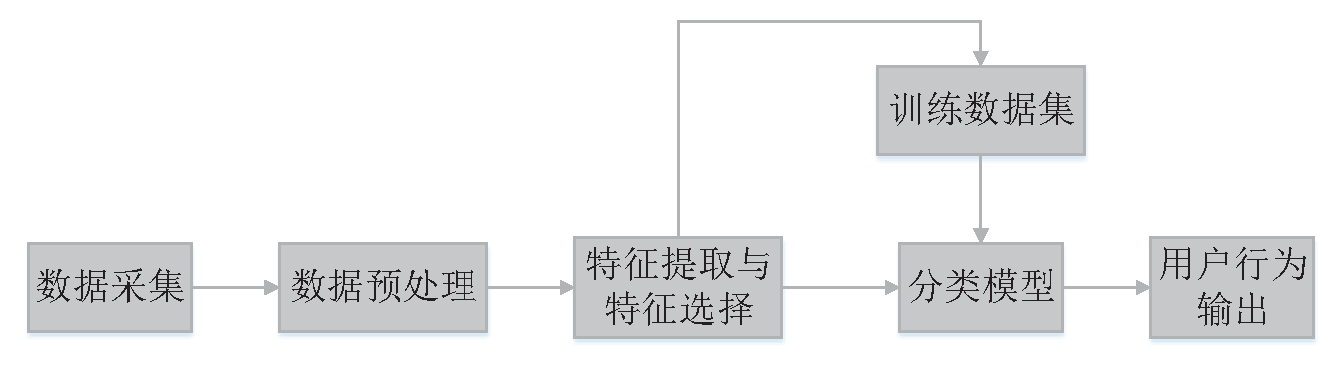
\includegraphics[width=0.8\textwidth]{basic_framework.eps}
\caption{行为识别基本框架流程图} \label{basic_framework}
\end{figure}

\par 近些年,随着智能手机的不断发展,其内部集成了越来越多的传感器,不仅包括在基于可穿戴传感器的行为识别中使用最多的加速度传感器,还包含有磁场传感器,陀螺仪等运动类型传感器,此外还有光照传感器,压力传感器,GPS等环境信息感知设备,可以获取充足的关于用户行为和环境信息。另一方面,智能手机的存储和计算能力也在不断提高与发展,其功能不断拓展与增强,这些就为基于智能手机进行行为识别提供了良好的硬件基础。伴随着智能手机的普及与应用,研究者也开始将重点关注到基于智能手机的行为识别技术。
\par 本章首先介绍智能手机内置的主要传感器以及其他感知设备,然后介绍在行为识别过程中必要的数据预处理步骤以及常用的特征提取和特征选择方法,最后详细介绍部分可以用于智能手机行为识别的分类模型和算法。

\section{数据采集}
\par 通过智能手机获取关于人体行为相关的数据一般都是通过智能手机内置传感器获取人体的加速度等信息,进而识别人体行为。本部分将首先介绍智能手机中常见的内置传感器,然后介绍智能手机中的数据采集模块。
\subsection{智能手机内置传感器}
\par 对于智能手机的内置传感器的介绍,本文以Android操作系统为例。Android操作系统是一种基于Linux的自由及开放源码的操作系统,主要用于移动设备,有Google公司和开放手机联盟领导开发。之所以选择Android系统为例介绍,一方面是因为Android是一款开源且成熟的移动端操作系统,另一方面它也也是目前市场占有量最大的手机操作系统,因此更具有代表性。对于传感器的集成以及为应用提供的传感器数据服务,其他操作系统也都十分类似,本节只是不是一般性地以Android系统为例介绍智能手机中的内置传感器。
\par Android系统平台支持的传感器类型很广泛,可以从功能和实现方式两个维度对其分类。一方面按照功能的不同,传感器可以分为运动类型传感器,环境传感器和方位传感器三类。运动类型传感器主要用于测量三轴向的加速度和角速度等,通常用于监测设备的移动,比如倾斜、震动、旋转或者摇摆等,主要包括加速度传感器、重力传感器、陀螺仪和旋转矢量传感器等。这一类型传感器在大部分智能手机内部都有集成,而且运动类型的数据也可以较好地用于人体行为识别。环境传感器则适用于测量各类环境信息参数,例如外界环境的温度、大气压强、光照强度和空气湿度等,主要包括温度传感器,气压传感器,温度传感器等。这一类型传感器在部分智能手机内有集成,可以检测人体周围环境信息,辅助人体行为识别,但是没有普适性。方位传感器主要用于测量设备的方向,主要包括磁场传感器和方向传感器,此外一般智能手机都集成了近距离创拿起,可以用于检测设备表面与物体的距离。
\par 另一方面按照实现方式的不同,传感器可以分为基于硬件和基于软件两类。基于硬件的传感器是集成在移动终端设备的物理实体。它们获得数据是通过直接测量特定的环境信息,比如加速度传感器,陀螺仪等。软件传感器是通过模拟硬件传感器,而并非真实的物理设备,它们是通过整合一个或多个硬件传感器信息相应数据,并通过一些融合方法计算获得相应模拟传感器的数据,因此也被称为虚拟传感器或者人工传感器,例如重力传感器,方向传感器等。Android平台所支持的传感器总结如表\ref{sensors}所示。

%传感器分类表
\begin{table}[htbp]
\centering
\caption{Android系统平台下内置传感器分类表} \label{sensors}
\begin{tabular}{|c|c|c|}
    \hline
    分类 & 基于硬件的传感器 & 基于软件的传感器 \\
    \hline
    运动传感器 & 加速度传感器,陀螺仪 & 线性加速度,旋转矢量传感器\\
    \hline
    环境传感器 & 光照传感器,气压传感器等 &  \\
    \hline
    方位传感器 & 磁场传感器,近距离传感器 & 方向传感器,重力传感器 \\
    \hline
\end{tabular}
%\note{这里是表的注释}
\end{table}

\par 下面本文详细介绍智能手机中常用于行为识别的传感器,包括加速度传感器,陀螺仪和磁场传感器。
\begin{itemize}
	\item 加速度传感器
\end{itemize}
\par 在Android系统平台下,存在加速度和线性加速度两类测量设备加速度,前者是基于硬件的传感器,又开发商生产直接集成在智能手机内部,产生原始的加速度数据,该数据包含重力加速度的影响。而后者则是基于软件的传感器,它是有加速度数据和其他类型传感器的数据融合后计算而得到的加速度信息,排除了重力加速度的影响。二者都会提供$x,  y,  z$三轴方向的加速度数据,其中加速度数据不仅提供加速度的大小(以$m/s^2$为单位),还提供了加速度的方向。对于每个轴向,加速度存在正值和负值分别表示两个相反方向的加速度。三个轴向的定义如图\ref{phone_orientation}所示。

\begin{figure}[ht]
\centering
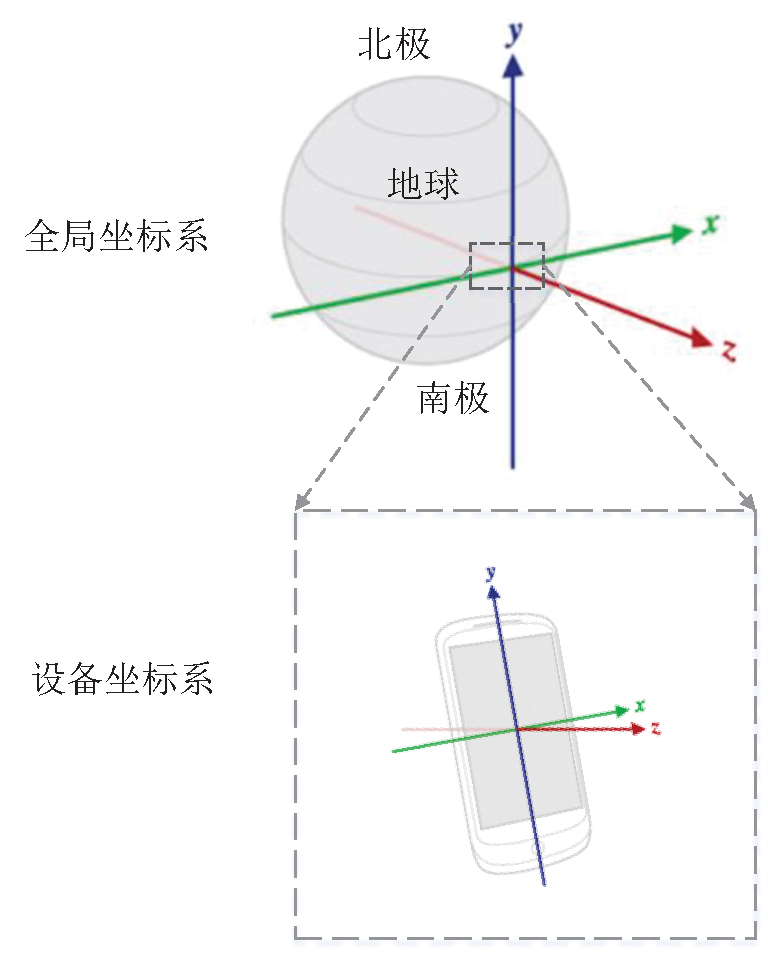
\includegraphics[width=8cm]{phone_orientation.eps}
\caption{Android全局和设备坐标系} \label{phone_orientation}
\end{figure}

\par 运动和方向传感器都是采集的矢量数据,数据的方向通常可以定义在直角坐标系中。Android系统平台定义了两个直角坐标系用以表征设备方向的相对变化。两个坐标系包括全局坐标系$x_E,  y_E,  z_E$ 以及设备坐标系$x,  y,  z$,其相对关系如图。图中表示了智能手机略微倾斜地放置在地球赤道上方时方向相对关系。在全局坐标系中$y_E$指向磁场北极,即接近正北方,$x_E$平行于地球表面,与$y_E$垂直,$z_E$指向正上方,即远离地心的方向。在设备坐标系中,$x$轴为水平方向,向右为正,$y$轴为垂直方向,向上为正,$z$轴为垂直于屏幕方向,屏幕正前方为正。几乎所有的三轴向的传感器都符合该坐标系包括下面会介绍的陀螺仪和磁场传感器,其所采集的数据均为全局坐标系中相应物理量在设备坐标系中三轴向的分解。
\par 加速度数据可以很好地表征不同行为的特点,加速度传感器在行为识别中也是应用最为广泛。基于可穿戴传感器的行为识别研究中,基于所有文献都是基于的加速度数据,而在智能手机中,加速度传感器集成也十分广泛,因此本文中它被选择为用于研究行为识别的传感器之一。

\begin{itemize}
	\item 陀螺仪
\end{itemize}
\par 陀螺仪是在设备发生旋转时,通过测量科氏(Coriolis)力测量设备在三个轴向上的角速度或旋转速度。所谓科氏力是指使得自由旋转物体从旋转参考系中看起来发生偏移的力。陀螺仪只能测量角速度,而不能直接测量旋转角度。但是可以通过陀螺仪的测量值在时间上的积分计算设备的旋转角度。陀螺仪的输出时绕设备坐标系的$x,  y,  z$三个轴向的旋转角速度值,单位为$rad/s$。如果坐标轴指向你自己,逆时针旋转则为正值,反之为负值。陀螺仪的示意图如图\ref{gyroscope}所示。

\begin{figure}[htb]
\centering
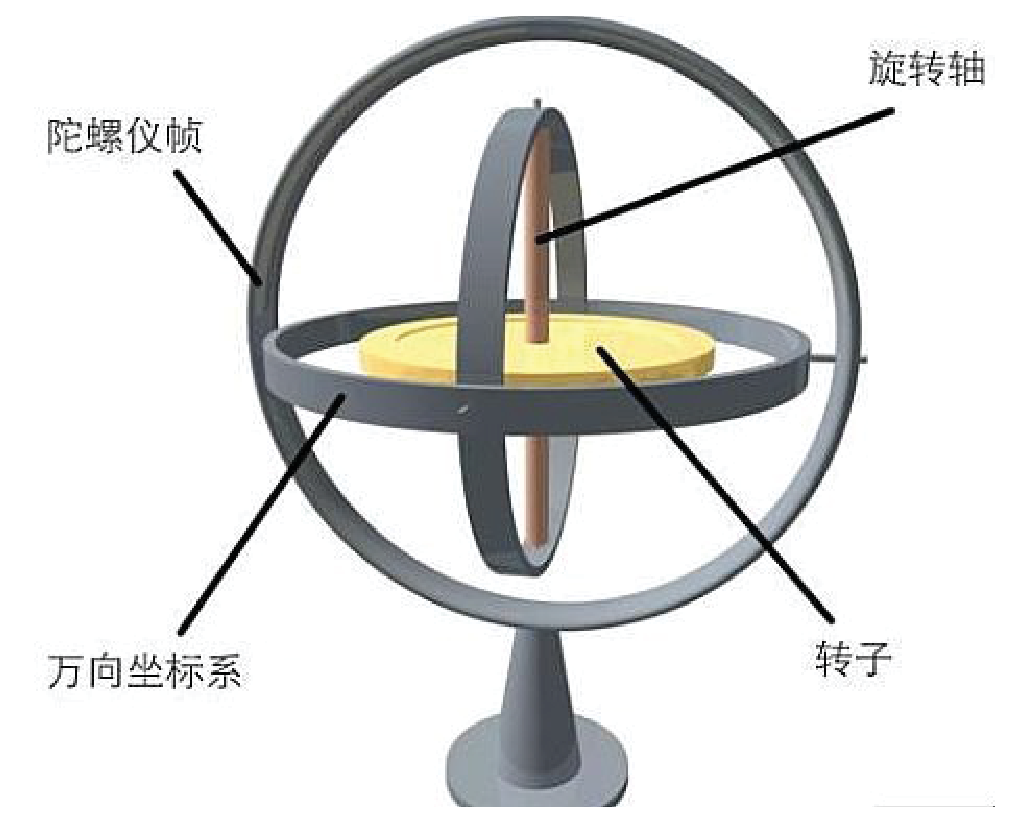
\includegraphics[width=8cm]{gyroscope.eps}
\caption{陀螺仪结构图} \label{gyroscope}
\end{figure}

\par 陀螺仪可以检测设备的旋转角速度,而在行为识别中,大部分的动态行为都是周期性行为,设备也会发生周期性旋转,所以通过处理陀螺仪数据可以很好地提取表征动态行为的特征,很好地辅助与行为识别。

\begin{itemize}
	\item 磁场传感器
\end{itemize}
\par 不同生产厂商的磁场传感器实现方式会有所不同。它们的实现方式主要可以分为基于霍尔效应、磁阻材料和洛伦兹力三种。其中霍尔效应传感器占据了最大的市场份额,在电流通过导线时,存在的磁场会使得导线两端的电子密度不同,从而形成正比于磁感应强度的电势差,通过电势差即可以计算出磁感应强度。磁场传感器也会以$x,  y,  z$三个轴向输出磁感应强度,因为集成的传感器是在每个方向上都有一个传感器。输出数据以微特斯拉$(\mu T)$为单位。
\par 磁场传感器的输出可以很好地判断设备方向的变化。在行为识别中,当行为发生转变时,磁场传感器的输出也会起到很好的辅助作用。

\subsection{智能手机数据采集模块}
\par 基于可穿戴传感器的行为识别中数据采集都是传感器将采集数据通过近距离通信的方式传送至中心节点,而基于智能手机的行为识别,其传感器和数据处理中心都是集成在手机内部,因此我们需要智能手机操作系统提供的编程接口,提取手机内置传感器的采集数据。Android系统提供了一系列的应用编程接口(Application Program Interface, API),方便获取传感器的数据。有关传感器的操作都有SensorManager负责统一管理。

\begin{itemize}
	\item 基本API
\end{itemize}
\par SensorManager时Android为便于应用访问传感器数据提供的系统服务。通过SensorManager一方面可以获取手机内置的传感器对象,用Sensor类表示设备种的传感器。另一方面通过SensorManager可以允许应用注册或注销传感器相关事件,并在注册成功后可以接受传感器数据。传感器事件可以通过注册的监听器SensorEventLitener监听。注册传感器事件以获取传感器数据,需要提供对于的Sensor对象,SensorEventListener对象和数据采集的采样时间间隔等。注册成功以后即可以通过定义的SensorEventListener中的回调方法获取传感器数据。

\begin{itemize}
	\item 传感器采样率
\end{itemize}
\par 在注册监听器时,通过指定监听器的采样间隔决定数据的采样率。在Android系统中,提供有四个常量表示采样间隔:SENSOR\_DELAY\_FASTEST ($0ms$,硬件传感器决定采样率),SENSOR\_DELAY\_GAME ($20ms, 50Hz$),SENSOR\_DELAY\_UI ($67ms, 15Hz$), SENSOR\_DELAY\_NORMAL ($200ms, 5Hz$)。同样也可以通过指定其他的事件间隔,即指定采样率注册事件监听器以获取相应传感器数据。

\begin{itemize}
	\item 传感器数据
\end{itemize}
\par Android系统中传感器的数据是以一个SensorEvent数据结构表示,并由传感器传递至应用定义在监听器SensorEventListener中的回调方法中,从而将传感器数据传回到应用中。SensorEvent包含以下属性用以保存数据:
\begin{itemize}
	\item SensorEvent.accuracy:表示传感器当前采集数据的精度
	\item SensorEvent.senor:表示采集该数据的传感器
	\item SensorEvent.timestamp:表示采集到该数据的时间
	\item SensorEvent.values:表示传感器的数据,以数组的形式保存三轴向的数据
\end{itemize}

\section{数据预处理}
\par 首先,虽然智能手机不断发展,其内置传感器也在一直改进,但是传感器采集数据依然存在着许多噪声干扰,需要对数据做平滑和均衡处理。其次,传感器采集的关于人体行为的数据是一个连续数据流,想要通过数据流识别人体当前的行为,必然需要将其分割成一个个的数据实例,才可以对其提取特征并进一步做分类处理。因此本小节将从低通滤波和数据分段两部分介绍数据预处理的基本内容

\subsection{低通滤波}
\par 对数据的平滑和均衡处理,主要是通过低通滤波的处理,有效减少数据中的高频噪声干扰。在移动终端这个条件下,通常会采用较为滤波方法,常见的简单滤波方法有加权平滑滤波和滑动平均滤波等。

\begin{itemize}
	\item 加权平滑滤波
\end{itemize}
\par 加权平滑滤波又称为一阶低通滤波,即每一个采样点的值通过上一个采样点的值与当前采样点的值取加权平均计算得到。加权平均可以实现有效阻断高频成分,保留低频信号,抑制周期性干扰,而且计算简便,易于实现。加权平均的计算公式为:
\begin{equation}
	Value[i] = Value[i-1]*(1-\alpha) + Data[i]*\alpha.
\end{equation}
其中Value表示我们计算得到的输出数值,Data表示采集的传感器数值,$\alpha$表示加权系数,决定了过去数值与当前采样数值的重要程度,位于0到1之间,起到平滑的作用。如图\ref{low_filter1}所示表示加权平滑滤波的效果。
\begin{figure}[htb]
\centering
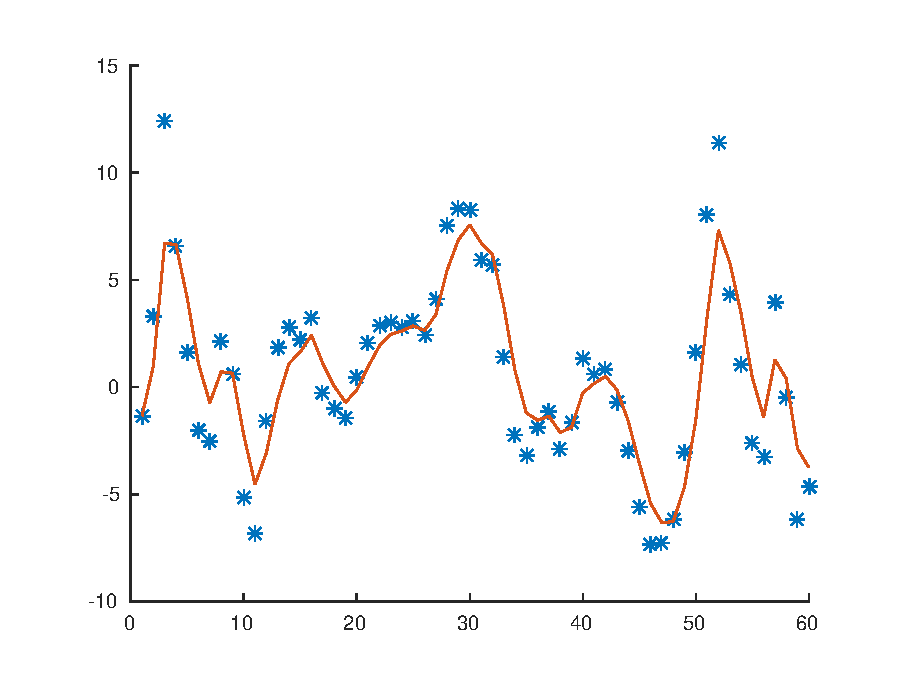
\includegraphics[width=0.6\textwidth]{low_filter1.eps}
\caption{加权平滑滤波} \label{low_filter1}
\end{figure}


\begin{itemize}
	\item 滑动平均滤波
\end{itemize}

\par 滑动平均滤波就是使用过去一段时间连续采集的传感器数据,通过平均处理以后作为每个点的输出数值。这是一种常见的数字滤波方法,可以有效消除波动,降低随机噪声的干扰。同样它的计算复杂度较低,容易理解和实现,其计算公式为:
\begin{equation}
	Value[i] = \frac{1}{W}\sum_{j=0}^{W-1}Data[i-j]
\end{equation}
其中,Value为输出数值,Data为传感器原始采样数据,W为选择的用于平均处理的窗口大小。在窗口移动过程中上述公式存在着重复计算问题,为了提高计算效率,充分利用之前的计算结果,可以通过推导递推公式改进计算方式,递推公式为:
\begin{equation}
	Value[i] = Value[i-1] + \frac{1}{W}(Data[i] - Data[i-W])
\end{equation}
如图\ref{low_filter2}所示表示滑动平均滤波效果图。
\begin{figure}[htb]
\centering
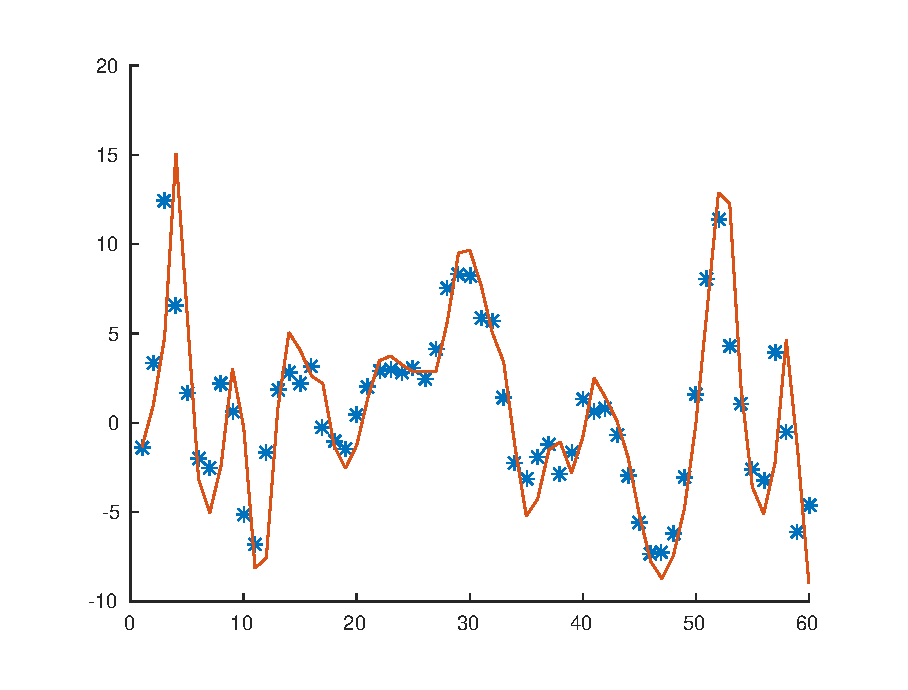
\includegraphics[width=0.6\textwidth]{low_filter2.eps}
\caption{滑动平均滤波效果图}\label{low_filter2}
\end{figure}

\subsection{数据分段}
\par 为从传感器数据流中识别人体当前的行为,有必要对连续的数据做分段处理获得行为数据实例。然后针对数据实例提取其中的部分特征进而才能通过分类算法识别出人体行为。所以分段的结果对识别结果会产生重要的影响,影响主要表现在识别准确率和识别实时性两方面。较长的数据段可以保证数据充分性提高识别准确率,而只有较短的数据段才可以保证一定的识别实时性,所以二者是一对矛盾体。为权衡二者的矛盾,重叠滑动窗口机制是在对连续数据流进行分段的常用方法。
\par 使用滑动窗口机制对数据做分段处理需要确定两个重要的参数,首先是窗口大小,其次是重叠比例。研究者通过对比实验研究了窗口大小对识别结果的影响程度。当窗口长度低于一定程度,识别准确率会随着窗口长度减小有明显下降趋势。另外一方面,重叠的比例也会影响识别实时性。较高的重叠比例可以在满足数据充分性的同时提高实时性,但是在行为转变过程中,识别反应过程就会变长,因此重叠比例也是一个需要重点考虑的参数。目前基于可穿戴传感器和基于智能手机的行为识别研究中,大部分的窗口长度都选择在3到10s之间,而重叠比例多数会选择50\%这样一个中间值。

\section{特征提取与特征选择}
\par 特征提取与特征选择对于行为识别是极其重要的一环,特征集的好坏直接决定了分类结果中识别准确率的高低。好的特征应当比较准确地表征某一类行为的一方面特点,同时该特征在不同行为之间应当表现出一定的区分度。因此,在分类之前,需要从连续的传感器数据流中提取出一系列的特征,同时还需要从这一系列特征中选择一个最佳的特征集,用于分类算法对该行为实例进行分类。本小节将从特征提取和特征选择两个步骤介绍它们通常用到的技术方法。

\subsection{特征提取}
\par 运动类型传感器所采集的关于人体行为的数据,通常都具有一定的波动性和周期性。因此基于传感器的行为识别,针对加速度等数据一般都会提取时域和频域特征,以及不同轴向数据的相关性,进而研究不同的行为特点。下面从时域和频域两个方面介绍常用特征。

\begin{itemize}
	\item 时域特征
\end{itemize}
\par 时域特征通过时域信号直接计算得到,计算简单,复杂度低。时域特征通常包括均值、均方根、方差、标准差、最值、相关系数等。

\par 均值($\overline{X}$)和均方根(Root Mean Square, RMS)描述了传感器数据在一个窗口时间内的平均大小,代表传感器数据的直流分量,体现了时域信号的低频特性。它们的计算公式如下:

\begin{equation}
	\overline{X} = \frac{1}{N}\sum_{i=1}^{N}x[i]
\end{equation}
\begin{equation}
	RMS(X) = \sqrt{\frac{1}{N}\sum_{i=1}^{N}x[i]^2}
\end{equation}
\par 方差($\sigma_X^2$)和标准差($\sigma_X$)描述了传感器数值分布的离散程度,体现了运动传感器信号的稳定性,方差计算公式如下,标准差为方差的算术平方根。

\begin{equation}
	\sigma_X^2 = \frac{1}{N-1}\sum_{i=1}^{N}(x[i]-\overline{X})^2
\end{equation}
其中,$\overline{X}$表示$X$轴向上窗口时间内传感器数据的均值,$N$为窗口时间内数据采样点数。
\par 相关系数($r_{XY}$)是一个常用统计量,常用于衡量变量之间的线性相关程度。传感器的不同轴向的数据之间的相关系数可以很好地表征行为的运动模式,可以用于区分不同的运动行为。$X$与$Y$轴的相关系数的计算公式如下:

\begin{equation}
	r_{XY} = \frac{\sum_{i=1}{N}(x[i] - \overline{X})(y[i] - \overline{Y})}{\sqrt{(x[i] - \overline{X})^2}\sqrt{(y[i] - \overline{Y})^2}}
\end{equation}
其中,$\overline{X}$和$\overline{Y}$分别表示$X$,$Y$轴向上窗口时间内传感器数据的均值,$N$为窗口时间内数据采样点数。
\par 此外时域特征还包括最大值、最小值、四分位距、分布直方图等,这里不再一一介绍。

\begin{itemize}
	\item 频域特征
\end{itemize}
\par 频域特征可以表现运动行为的周期性特点,通常需要先对时域信号做快速傅里叶变换(Fast Fourier Transform, FFT),然后再对频域信号计算频域特征值。频域的特征通常包括频域的最值、频谱能量、频域熵、功率谱密度等。
\par 频谱能量($Energy$)描述运动状态下,传感器信号的周期特性,其计算方式为对快速傅里叶变换后的频谱序列各个分量的幅度计算平方和,其计算公式如下:
\begin{equation}
	Energy(X) = \frac{\sum_{i=1}^{N}|F_i|^2}{N}
\end{equation}
其中,$|F_i|$是信号频谱中的第$i$个分量的幅度。
\par 信息熵($Entropy$)描述信号频谱特征,其计算方式同样是对快速傅里叶变换后的频谱序列,对其求取信息熵,反应频谱的分布特征,其计算公式如下:
\begin{equation}
	Entropy(X) = \sum_{i=1}^{N}(-p_ilogp_i)
\end{equation}
其中,$p_i$表示信号频谱中第$i$个分量在频谱中所占的比例。
\subsection{特征选择}
\par 通过一系列的特征计算,可以组成关于一段窗口时间内数据的特征向量。如果特征向量中特征数量太多,一方面需要消耗大量的计算资源,另一方面还会在训练分类模型中造成过拟合导致人体行为识别准确率下降。因此我们需要从可选特征向量中选择最佳特征集用于训练分类模型以及行为实例的分类。特征选择方法很多,使用较为广泛的主要包括主成分分析法,线性判别分析法以及根据信息增益特征排序选择方法等。
\par 主成分分析(PCA),就是通过正交变换,将原来存在一定相关性的特征向量变换为在分量上不相关的随机向量。具体地,首先计算特征向量的协方差矩阵而转换为一个对角矩阵,然后对其做正交变换,将其变换到$p$个正交方向,从而将多维的特征向量降为低维向量,而且尽可能多地保留信息,从而达到降维的效果。
\par 线性判别分析法(LDA),其基本思想是将高维的特征向量映射到最优的矢量空间,然后抽取分类信息以及降低特征空间的维数。通过映射以后的特征空间具有最优的可分离性,在新的子空间中具有最小的类内距离和最大的类间距离。最终在降低特征维度以后获得最佳的分类效果。
\par 另外一种常用的方法就是使用有监督的方法计算每一维特征的信息增益或信息增益比,进而对所有特征排序,然后选择信息增益或信息增益比最大的若干特征组成特征集。信息增益(information gain, IG),其计算公式如下:

\begin{equation}
	Entropy(t) = -\sum_{i=1}^{c}p(i|t)log_2p(i|t)
\end{equation}
\begin{equation}
	IG = Entropy(parent) - \sum_{j=1}^{k}\frac{N(v_j)}{N}Entropy(v_j)
\end{equation}
其中,$Entropy(.)$表示信息熵,$t$表示记录总数,$c$表示类别总数,$p(i|t)$表示类型$i$记录数所占的比例;在公式2.10中,$k$表示属性值的个数,$N$表示记录总数,$N(v_j)$表示按照某特征分类,实例被分为$j$类的实例数量。因此信息增益其实就是按照某一个特征对所有实例分为$k$类,分类前后信息熵的差值。
这种方法计算简单且易于理解,尽可能地保留了特征空间中不同类别行为之间的区分度,选择的特征集可以较好地用于分类模型。

\section{分类算法}
\par 所谓人体行为识别就是根据一定时间的行为特征判断这段时间最有可能的行为,可以将其归结为分类问题。从数据挖掘和模式识别的角度看,行为识别就是一个多分类的问题。在模式识别领域存在着诸多的成熟分类算法,本小节将从基础分类算法和提升分类算法两部分介绍常用于人体行为识别的分类算法。

\subsection{基础分类算法}
\par 基础分类算法由于其算法简单易于实现,而且算法复杂度较低,因此需要在智能手机终端对行为作出识别判断的研究中,这类算法应用特别广泛。常用于基于智能手机的行为识别研究中的基础分类算法主要包括K-近邻分类算法,朴素贝叶斯算法,决策树和支持向量机等。

\begin{itemize}
	\item K-近邻分类算法(K-Nearest Neighbor, KNN)
\end{itemize}
\par K-近邻分类算法是一种有监督的惰性机器学习算法。该算法简洁且易于理解,其基本思想就是在特征空间中定义一种实例之间的距离,使用最多的时欧氏距离,当有实例需要判定类别时,在所有实例中按照定义好的特征空间距离寻找K个与之距离最短的实例,根据这K个实例的标签决定该实例的类别。KNN的算法的优点是简单易于实现,且不需要训练分类模型,但也有一定的缺点。使用KNN必须保存一定数量的实例,占用一定的存储空间,而且它是一种惰性分类算法,需要在识别时计算实例之间的距离,可能会对识别实时性造成一定影响。
\begin{itemize}
	\item 朴素贝叶斯分类算法(Naive Bayesian)
\end{itemize}
\par 朴素贝叶斯分类算法是基于贝叶斯定理之上实现的有监督的学习算法,贝叶斯定理如下:
\begin{equation}
	P(H|X) = \frac{P(X|H)P(H)}{P(X)}
\end{equation}
其中,$H$表示一种假设,在分类模型中表示分为某一类的假设,$X$表示支持该假设的证据,在分类模型中表示特征向量的某一个特定取值组合, $P(X)$和$P(H)$时$X$和$H$的先验概率,$P(X|H)$是在$H$条件下$X$的条件概率。
\par 朴素贝叶斯分类算法的基本假设是所有特征彼此独立。因此条件概率可以同以下方法计算:
\begin{equation}
	P(X|H) = \prod_{k=1}^{n}P(x_k|H)
\end{equation}
其中,$x_k$表示第$k$个属性的值。
由于先验概率容易获得,而条件概率计算以后就可以计算获得一个特征组合下,每一个假设分类的后验概率,通过比较选择最大后验概率即可获得分类结果。朴素贝叶斯分类算法同样简单易于实现,但是最大的限制就在于对特征彼此独立的假设条件。

\begin{itemize}
	\item 决策树(Decision Tree)
\end{itemize}
\par 决策树是一种有监督的学习分类算法,其分类的流程实例如图\ref{decision_tree}所示。决策树的每个叶节点代表一个类别,每个分支代表一个组属性值组合。决策树的建立时基于实例数据的信息熵。每一步的数据实例分裂都选择使得信息增益或信息增益比最大的特征将数据实例分裂为若干类,直到将所有实例都分类。为了避免出现过拟合,决策树中还可以通过剪枝的方法泛化模型。决策树最大的优势就是易于理解分类规则,易于实现,而且不依赖于特征的独立性,所以较为广泛地应用在行为识别当中。

\begin{figure}[!htb]
\centering
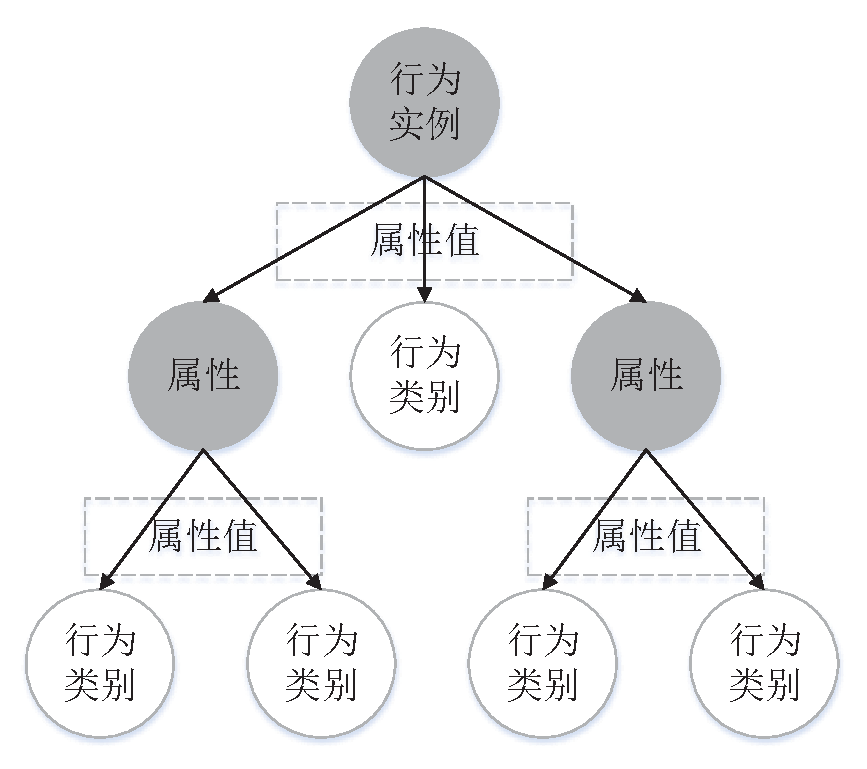
\includegraphics[width=8cm]{decision_tree.eps}
\caption{决策树分类算法流程图} \label{decision_tree}
\end{figure}
\begin{itemize}
	\item 支持向量机(Support Vector Machine, SVM)
\end{itemize}
\par 支持向量机是一种最为常用的有监督学习算法,它通过计算一个或多个高维的超平面将实例数据分割成多个类,其原则是使得超平面与支持向量的间隔最远。对于线性可分情况,可以直接计算超平面用于分类,对于线性不可分情况可以使用非线性映射算法将低维输入线性空间映射到高维的特征空间,使其线性可分,然后求解超平面对其进行分类。支持向量机同样广泛应用与行为识别,姿势识别等领域。

\subsection{提升分类算法}
\par 由于智能手机的计算能力有限以及行为识别对实时性的要求,基于智能手机的行为识别研究中,提升的分类算法应用并不太广泛,这里只介绍随机森林分类算法。随机森林计算相对简单,复杂度相对较低,而且一些研究者也通过实验表明该学习方法在行为识别中取得了很好的效果。
\begin{itemize}
	\item 随机森林分类算法(Random Forest)
\end{itemize}
\par 随机森林分类算法是决策树的一种组合形式。在随机森林的建立阶段,从$M$个特征中随机选择$m$个特征,其中$m<<M$,使用这$m$个特征建立决策树,其过程与独立决策树完全相同。多次执行相同过程,这些随机选择特征集的决策树就组建成了随机森林。在决策分类阶段,实例会通过每一棵决策树进行分类,最终的结果由所有决策树的分类结果投票决定。
\par 随机森林在建立阶段一方面由于随机选择少量特征,不容易出现过拟合,而且训练速度较快,计算复杂度相对较低,另一方面是从特征集中随机选择特征,因此也可以用于高维特征数据实例的分类,而且对特征选择的要求不高。同时,在决策分类阶段,由于综合了多个决策树的结果,在准确率上有了很大的提高,在应用到行为识别上,这一点在文献中通过实验获得了证实。

\section{本章小结}
\par 本章简要介绍了基于智能手机行为识别的相关技术。首先简要概述了智能手机中内置传感器种类和功能以及手机的数据采集模块。然后介绍了数据预处理方法,包括低通滤波和数据分段处理,同时介绍了行为识别中常用特征以及特征选择方法。最后介绍了可以用于基于传感行为识别的分类算法

  %自行添加!
  \chapter{基于智能手机的两层多策略行为识别框架}

\par 在人体行为识别的基础之上的应用极为广泛,它们可以给现代人的娱乐生活、医疗健康等诸多方面带来极大的便利与帮助。而对于此类应用,准确地感知和识别用户姿势或行为是其中最为关键的核心任务。为了感知和识别用户行为,首先需要比较方便并且具有较少用户侵入性地采集有关人体的行为数据,其次需要设备具有能力传输或者处理数据,进一步判断和识别用户行为。近些年随着智能手机的不断发展,仅仅通过智能手机这一个设备已经具备了上述条件。首先智能手机内部集成有多种传感器,可以很好地采集用户的运动信息,其次智能手机的应用越来越广泛,其与现代人的关系也愈加密切,因此它可以方便且无侵入性的长期监测用户的运动信息。最后智能手机的存储和计算能力不断增强,现在已经完全可以应对提取特征,运行分类算法等复杂计算,因此可以很好地完成识别任务,且避免了传感器数据通信的麻烦。
\par 基于智能手机进行行为识别,不仅应用方便灵活,而且研究者也通过实验表明内置的多种类型传感器可以有效提高识别准确率。未来随着智能手机的不断进步和发展,基于智能手机的行为识别具有良好的应用前景。然而,智能手机在使用方便灵活的同时也存在着其他的问题。由于它的不固定性,其位置和方向的变化会对内置传感器所采集的运动数据产生很大干扰,对最终的识别结果影响较大。因此我们需要提出新的解决方法降低这方面的影响。
\par 为解决上述问题,本章提出一种基于智能手机的两层多策略行为识别方案框架,其流程框图如图\ref{framework}所示,框架主要包括数据获取,分组算法和多策略分类三部分。首先多个传感器以固定的采样率采集关于人体的行为数据信息。同时为了可以实现实时地行为识别,本文采用带有重叠的滑动窗口机制对智能手机所采集的传感器数据分割为固定窗口时间长度的数据段,然后对于每一段数据提取若干行为特征组成特征向量。基于这一特征向量,根据不同的行为分类问题通过信息增益排序的方式选择最佳特征子集用于训练相应的分类器并使用该分类器完成最终的分类任务。在本文的框架中,行为分类由两层组成,首先在第一层中为分组模型,即根据行为之间的相似程度被分为若干组。然后在第二层中根据不同组的行为的不同特点使用不同策略和相应的最佳分类器进行最后的分类。
\begin{figure}[ht]
\centering
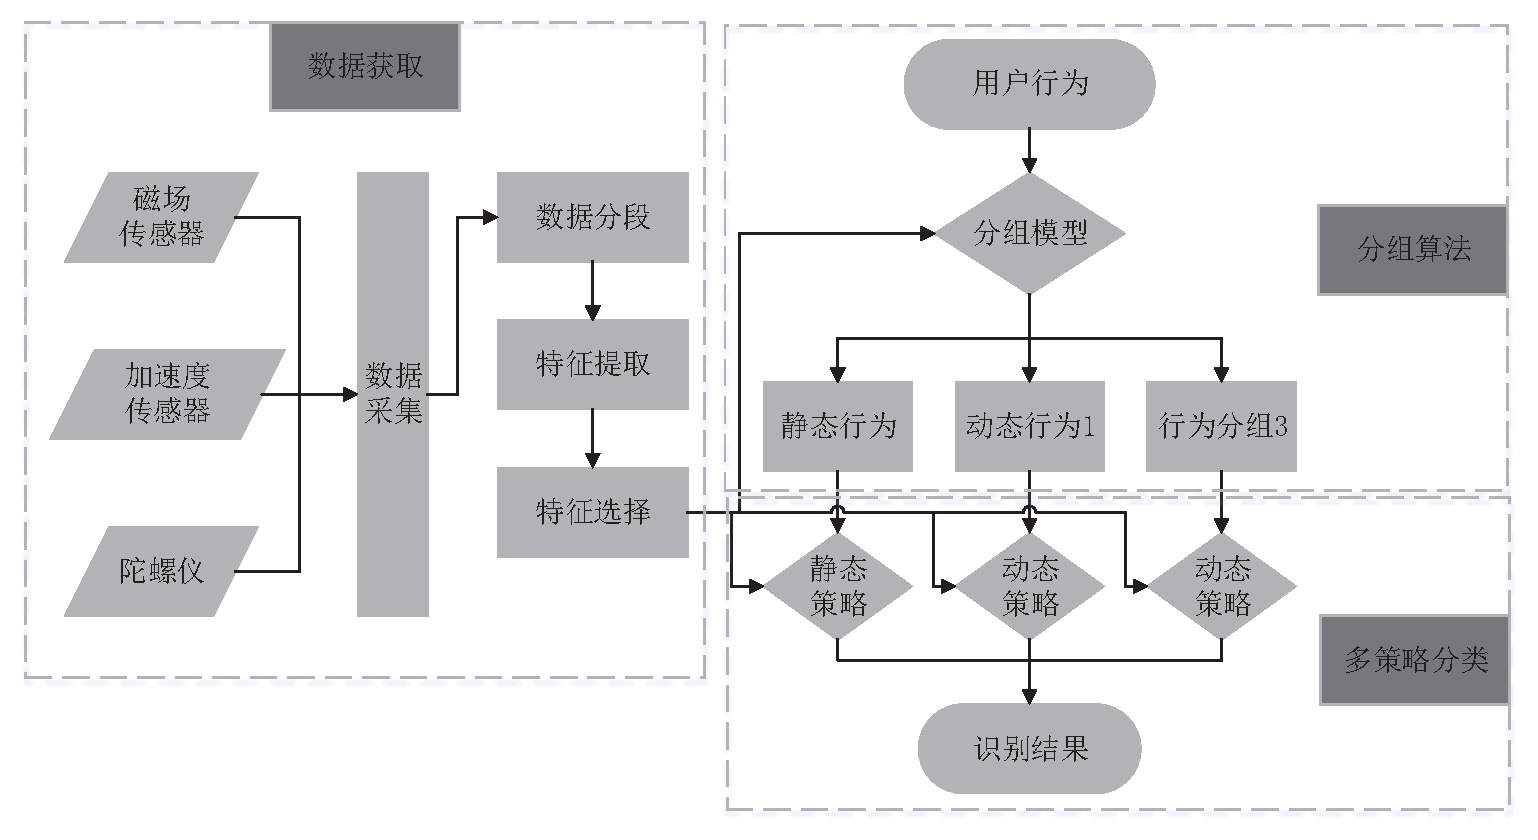
\includegraphics[width=1.0\textwidth]{framework.eps}
\caption{两层多策略的行为识别框架流程图} \label{framework}
\end{figure}

\section{数据获取与特征提取}
\par 该部分的主要作用是为分类模型提供以特征向量为基本形式的训练集和测试集数据,主要包括传感器数据的采集与预处理,特征提取与特征选择两个操作步骤,前者负责数据获取并处理为数据实例,后者则负责将数据实例转换为一维特征向量,为进一步训练分类模型以及测试分类做准备\scite{wu2012classification}\scite{gupta2014feature}。
\subsection{数据采集与预处理}
\par 在本文的框架中,首先数据集来自三类传感器,包括加速度传感器,陀螺仪和磁场传感器。之所以选择这三个传感器,一方面是因为在文献\cite{diffSensors}中 作者已经通过实验验证了它们对行为识别的有效性,另一方面时因为目前几乎所有手机都有集成这三类传感器,这也可以保证行为识别技术应用的广泛性。每个传感器都以固定采样率$f$采集数据获得连续数据集。然后针对连续数据集,经过低通滤波后,采用长度为$T$以及重叠为50\%的滑动窗口对数据进行分割,最后每一段数据生成一个四维的信号向量$(x, y, z, magnitude)$, 基于数据向量就可以进行提取特征。 其中:
\begin{equation}
	magnitude = \sqrt{x^2+y^2+z^2}
\end{equation}
\par 最后选择加入三轴方向的信号模值在一定程度上可以降低方向变化对行为识别的干扰。

\subsection{特征提取与特征选择}
本文中所使用的全部特征列举在表格\ref{feature_list}中, 主要包括时域的特征、频域的特征和关于自相关函数的特征。

\begin{table}[!htb]
    \caption{本文所使用的特征列表} \label{feature_list}
    \begin{tabular}{|c|c|c|c|c|c|}
    \hline
    类别 & 特征名称 & 符号 & 类别 & 特征名称 & 符号 \\
    \hline
    \multirow{4}{*}{时域特征} & 信号均值 & $\mu (\textbf{x})$ & \multirow{6}{1cm}{自相关函数特征} & 自相关最大值 & $R_M$ \\
    \cline{2-3} \cline{5-6}
    & 信号方差 & $\sigma ^2 (\textbf{x})$ & & 极大值的间隔 & $I$  \\
    \cline{2-3} \cline{5-6}
    & 窗口差值 & $\mu T$ & & 差分值 & $Diff$ \\
    \cline{2-3} \cline{5-6}
    & 窗口偏差 & $\mu D$ & & 中间部分的最大值 & $Mid_M$ \\
    \cline{1-3} \cline{5-6}
    \multirow{3}{*}{频域特征} & 最大分量 & $F_f$ & & 中间部分的最小值 & $Mid_m$ \\
    \cline{2-3} \cline{5-6}
    & 最大分量的模值 & $A_f$ & & 中间部分的均值 & $Mid_{\mu}$ \\
    \cline{2-6}
    & 能量值 & $E$ & & & \\
    \hline
    \end{tabular}
\end{table}


下面以向量$\textbf{x}$为例说明上述系列特征的细节,其中向量$\textbf{x}$的长度为$N$。
\begin{itemize}
	\item 时域特征
\end{itemize}
\par 时域特征包括均值和方差等,计算简单并且可以有助于区分静止和动态行为\scite{positionClassifier},其中窗口差值和窗口偏差计算公式如下:

\begin{equation}
	\mu T = \sum_{i=2}^{M}(|\mu_i - \mu_{i-1}|)
\end{equation}
\begin{equation}
	\mu D = \sum_{i=1}^{M}(|\mu_i - \mu|)
\end{equation}

其中, 窗口长度为$N$的向量$\textbf{x}$被分割为$M$段,$\mu_i$表示第$i$段数据的均值,$\mu$表示向量$\textbf{x}$的均值。

\begin{itemize}
	\item 频域特征
\end{itemize}

\par 本文中频域信号主要是通过快速傅里叶变换(Fast Fourier Transform, FFT)算法计算得到得。在频域中,我们重点关注最大频域分量以及频域的能量分布。频域特征与位置信息相关性较小,位置敏感度低,因此可以用来区分动态行为,而受到来自位置变化的影响较小。
\begin{itemize}
	\item 自相关函数特征
\end{itemize}
\par 信号的自相关函数可以通过公式3.4计算得到。其中加速度数据和陀螺仪数据信号的自相关函数的图像分别如图\ref{three_dimen}(a)和\ref{three_dimen}(b)所示。
\begin{equation}
	R_x[i]=\frac{1}{N}\sum_{j=i}^{N-1} x[j]x[j-i]\qquad  i=0, 1, \cdots, N-1
\end{equation}
\begin{figure}[!htb]
    \centering
    \subfloat[加速度信号的自相关函数]{
    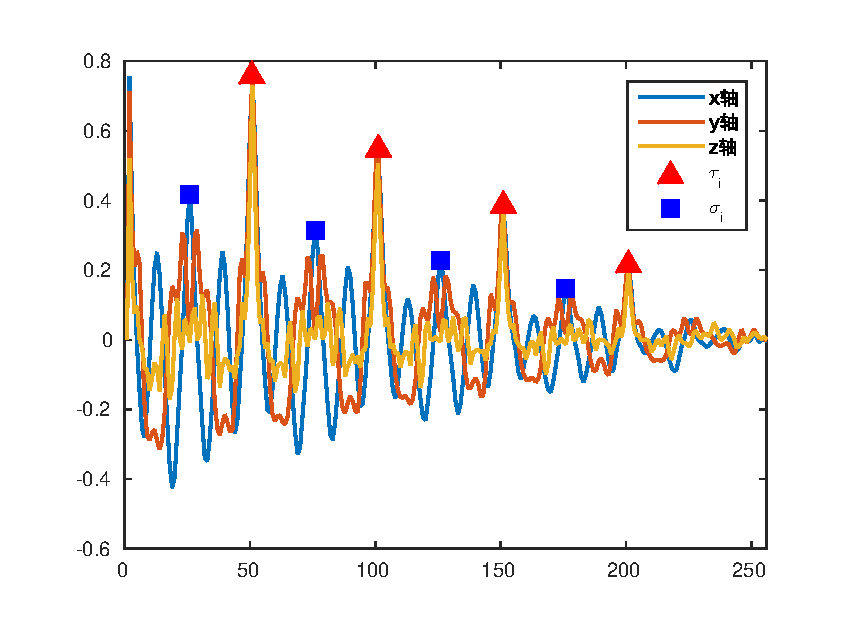
\includegraphics[width=0.45\textwidth]{three_dimen_acc.eps}}
    \subfloat[陀螺仪数据的自相关函数]{
    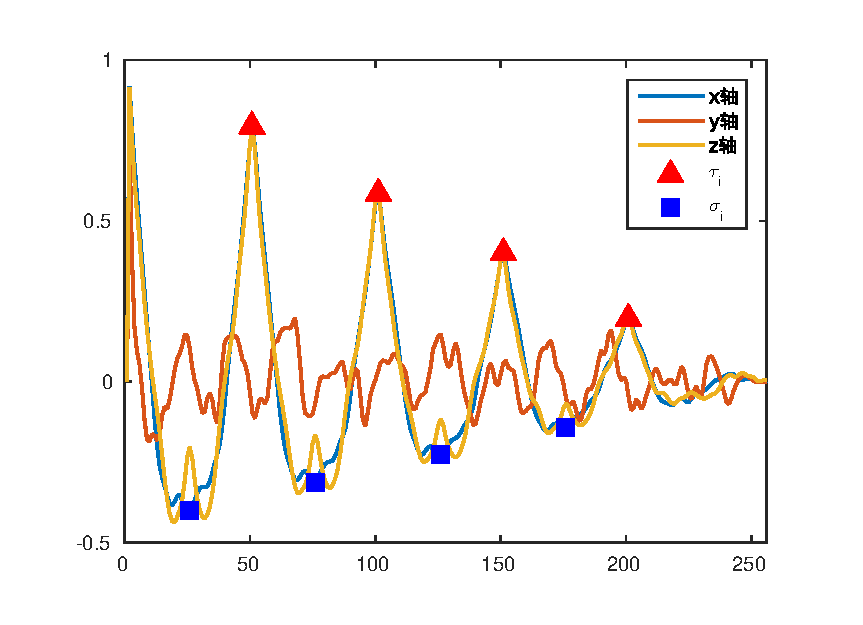
\includegraphics[width=0.45\textwidth]{three_dimen_gyro.eps}}
    \caption{传感器三维数据的自相关函数} \label{three_dimen}
\end{figure}

\par 如图\ref{three_dimen}所示,传感器数据三维信号的自相关函数在同一点取得极值,我们记为 $\tau_i$,表示自相关函数的第$i$个极值。由于加速度传感器和陀螺仪是集成在同一部智能手机当中,因此他们所采取的数据计算相关函数极值的位置也相同。如果将它们各自的三维自相关函数加在一起就可以使得极值更加明显,不易被噪声混淆。另外使用自相关函数的和而非使用三轴向的传感器数据各自提取特征可以有效减少因为方向变化带来的影响。因此,在本文中关于自相关函数的特征都是使用自相关函数之和,即$R = R_x + R_y + R_z$,而不是每一维数据的自相关函数。

\begin{figure}[!htb]
    \centering
    \subfloat[加速度信号的自相关函数]{
    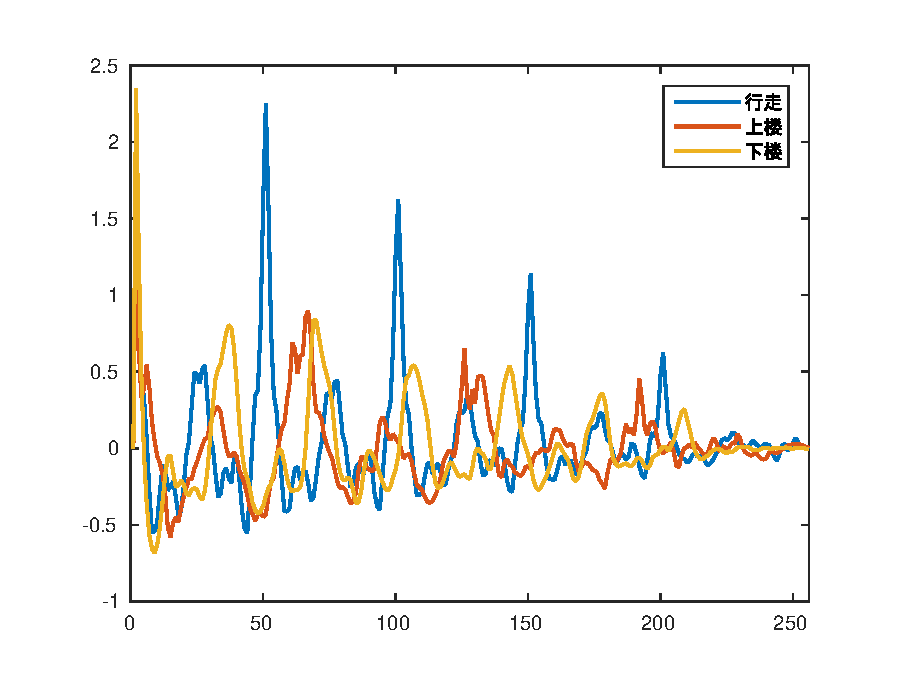
\includegraphics[width=0.45\textwidth]{acti_acc.eps}}
    \subfloat[陀螺仪数据的自相关函数]{
    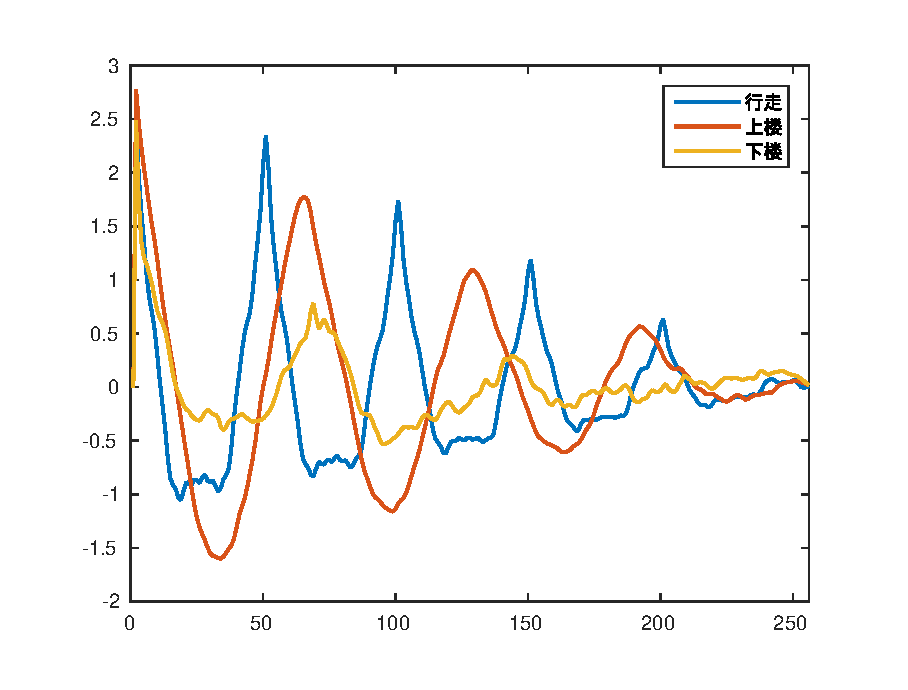
\includegraphics[width=0.45\textwidth]{acti_gyro.eps}}
    \caption{相同位置下不同行为时数据自相关函数}
\end{figure}

\begin{figure}[!htb]
    \centering
    \subfloat[加速度信号的自相关函数]{
    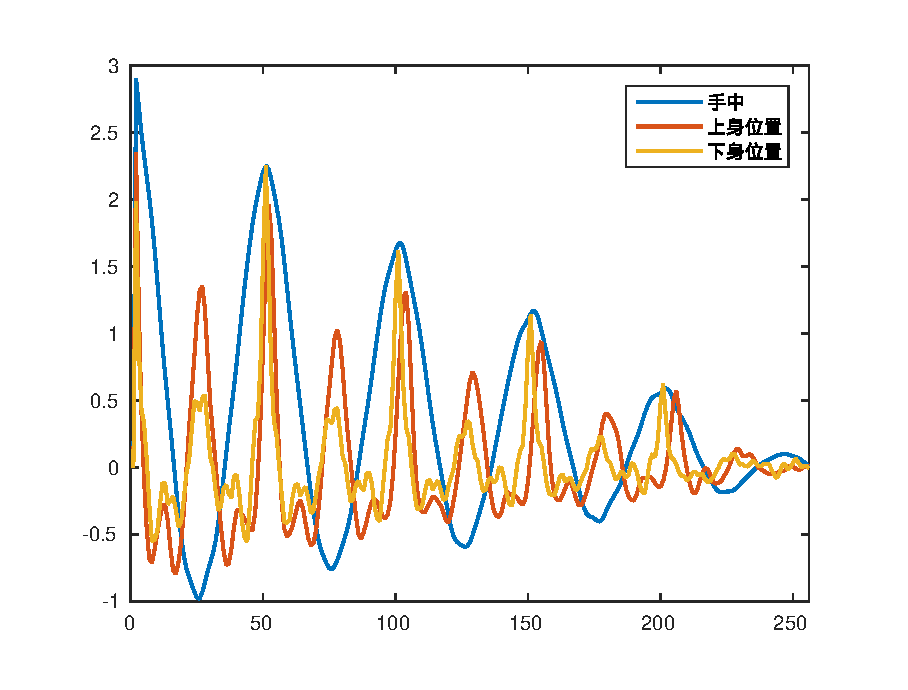
\includegraphics[width=0.45\textwidth]{posi_acc.eps}}
    \subfloat[陀螺仪数据的自相关函数]{
    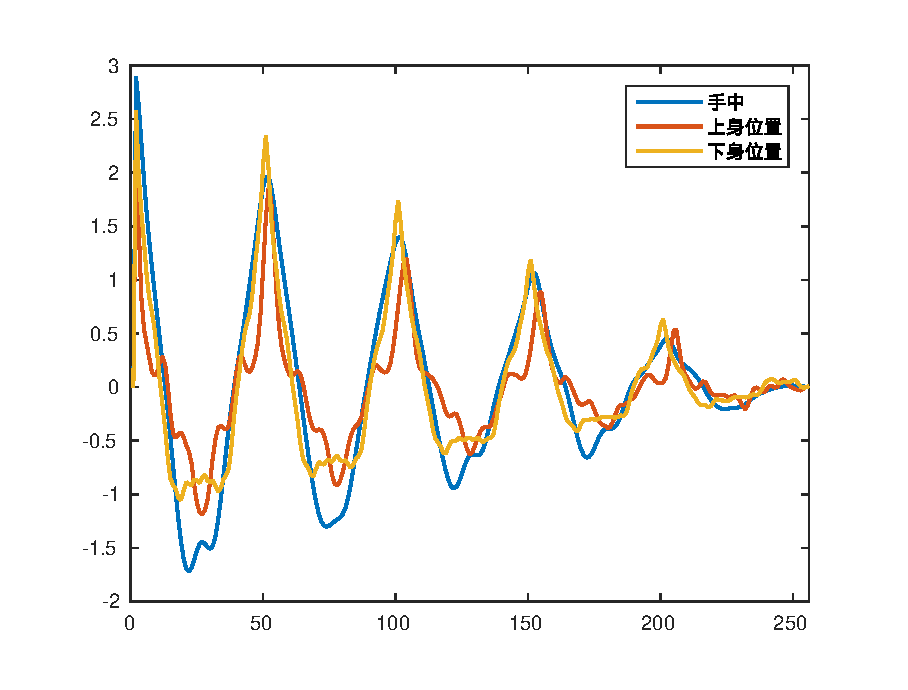
\includegraphics[width=0.45\textwidth]{posi_gyro.eps}}
    \caption{行走状态下不同位置时数据自相关函数}
\end{figure}

\par 使用自相函数的和计算以下特征,其中本文中使用前m个极值,计算公式分别如下:
\begin{equation}
    R_M = \frac {1}{m}\sum_{i=1}^m R[\tau_i]
\end{equation}
\begin{equation}
    I = \frac{1}{m}\sum_{i=1}^m {(\tau_i-\tau_{i-1})}
\end{equation}
\begin{equation}
    Diff = \frac{1}{m}\sum_{i=1}^m \sum_{j=\tau_i-3}^{j=\tau_i+3} {|R[j]-R[j-1]|}
\end{equation}
\par 关于自相关函数的其他特征都与相邻极值中点$\sigma_i$ 处的函数值有关。在本文中,自相关函数相邻极值中点$\sigma_i$ 附近的一系列函数值被抽象为一个向量,比如 $\textbf{r}=\frac {1}{m} \sum_{i=1}^m\{R[j]\}, j=\sigma_i-3, \sigma_i-2,\cdots,\sigma_i+3$。这一向量的最大值、最小值和平均值被作为本方案中最后三个特征,分别表示为$Mid_M$, $Mid_m$, $Mid_\mu$。关于自相关函数的特征具有方向独立性的特点,因此可以有效区分动态行为而受到来自方向变化的影响较小。
\par 在本方案中使用的三个传感器,时域和频域特征从四维数据中提起包括三轴方向和模值,即$d=\sqrt{x^2+y^2+z^2}$,共组成84维特征向量。而自相关函数的特征则是提取自加速度传感器和陀螺仪的三轴方向的自相关数之和,即组成12维自相关函数特征集。因此最终的特征向量共有96维,然后对于不同的分类任务,分别计算这些特征的信息增益并排序,最终为不同的分类问题选择最佳特征集。通过为不同分类任务选择维数较小的特征数量,不但可以有效减少特征计算的复杂度,而且可以有效利用不同特征在不同分类问题中的优势。

\section{分类模型}
\par 本文中的方案框架将分类模型分为两层,第一层为分组模型,主要负责将行为分类至某一组,组内的行为相似度高,不易区分,但是组间的区分度较大,易于分类,不易受到干扰因素的影响,误差率低\scite{ustev2013user}。分类模型的第二层则是针对不同组行为的特点,采用对应最佳策略对其进一步分类。在本文中,考虑静态和动态两类行为分类策略。由于静态行为在运动传感器数据中没有明显特征,因此本文考虑借助于识别过程中的过渡态行为进一步判断静态行为。而对于动态行为,容易受到来自位置变化的影响,本文方案中考虑使用位置分类器识别位置信息,然后在不同位置训练特定分类器对动态行为进一步分类。
\subsection{分组模型}
\par 实际生活中一些行为之间的区分度十分明显,比如静止和跑步,即使存在位置和方向变化的干扰,也可以很容易的区分这些行为\scite{lu2010jigsaw}。因此在本文方案中,所有行为将根据行为之间的差异程度首先分为若干组,在识别过程中,所有行为可以利用第一层分类器判决他们属于哪一个组。行为的分组结果的获取是首先通过一个简单的分类方法对测试数据集进行分类,并根据行为的混淆矩阵计算行为之间的行为相似度。行为之间的相似度定义如下:
\begin{equation}
    \omega_{ij}=\frac { c_{ij}+c_{ji} }{ c_{ii}+c_{ij}+c_{ji}+c_{jj} }
\end{equation}
其中,$c_{ij}$表示在行为分类混淆矩阵中,行为$i$的实例被分类器分为行为$j$的数量。
\par 然后所有的行为可以根据上述公式计算出的行为相似度进行分组,分组的结果应满足以下原则:
\begin{equation}
    \begin{aligned}
    &(1) \bigcup_i A_{group-i}=A \\ \
    &(2) A_{group-i}\bigcap A_{group-j}=\phi,\: i\neq j \\ \
    &(3) \forall a\in A_{group-i},\: \exists b\in A_{group-i}\wedge b\neq a, \: \omega_{ab} \geq \lambda_\omega\\ \
    &(4) \forall a\in A_{group-i},\: \forall b\in A_{group-j}\wedge i\neq j, \: \omega_{ab} \leq \lambda_\omega
    \end{aligned}
\end{equation}
\par 在本文中,行为集共包括六类不同行为,包括坐(ST),站(SD),行走(WK),跑步(RN),上楼(AS)和下楼(DS)。本文所提出的框架并不局限在这六种行为,框架可以很好地扩展应用到其他行为。根据训练集数据,我们选择信息增益最大的前10个特征和决策树的分类方法对行为分类。这里相似度的阈值设置为 $\lambda_\omega = 0.05$。通过交叉验证的方法可以从识别结果中得到混淆矩阵,进而计算出不同行为之间的相似度,相似度的结果如图\ref{similarity}所示。
\begin{figure}[!htb]
\centering
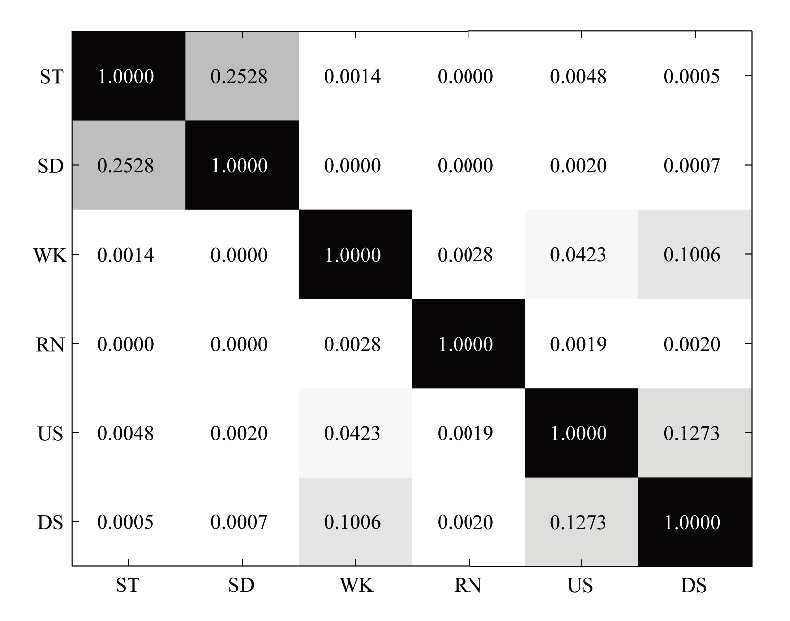
\includegraphics[width=0.6\textwidth]{similarity.eps}
\caption{行为之间的相似度}\label{similarity}
\end{figure}

\par 根据行为相似度以及分组原则,行为的分类结果如表格\ref{group_result}所示,此结果也刚好符合我们正常的思维习惯。

\begin{table}[!htbp]
\centering
\caption{行为分组结果}\label{group_result}
\begin{tabular}{cc}
\toprule
类型& 行为\\
\midrule
\multirow{2}*{静止行为}
&坐(Sitting, ST)\\
&站(Standing, SD)\\
\hline
\multirow{3}*{慢速动态行为}
&行走(Walking, WK)\\
&上楼Ascending Stair, AS)\\
&下楼(Descending Stair, DS)\\
\hline
\multirow{1}*{快速动态行为}
&跑步(Running, RN)\\
\bottomrule
\end{tabular}
\end{table}

\subsection{静态行为分类策略}

\par 对于静态行为,比如坐和站的状态,它们的运动特征几乎没有区别,因此根据加速度等信息很难区分它们。另外,也不能像基于可穿戴传感器的行为识别中使用方向信息进行判断,因为手机并不是相对于人体是固定不变的。为此,在本文中我们提出一种间接的策略区分静态行为,即引入过渡行为状态。比如,对于区分坐和站,过渡包括坐下和站起等,可以帮助区分两类静止行为。图\ref{transfer}(a)是当手机分别放置在上身和下身位置时,实验参与着周期性坐下和站起时陀螺仪的时域信号。从图中可以看出在持续静止状态下很容易可以通过陀螺仪检测到两个过渡状态,而且二者的区别也十分明显,容易通过运动特征区分两种过渡状态行为。另外一方面图\ref{transfer}(b)是实验参与者在周期性行走、坐下和站起时陀螺仪的时域信号。

\begin{figure}[!htb]
    \centering
    \subfloat[周期性站起和坐下时的时域信号]{
    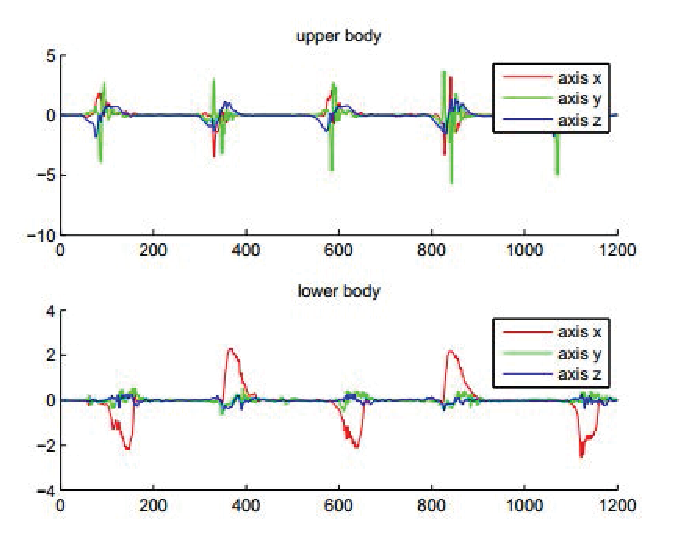
\includegraphics[width=0.45\textwidth]{transfer1.eps}}
    \subfloat[周期性坐下、站起和行走时的时域信号]{
    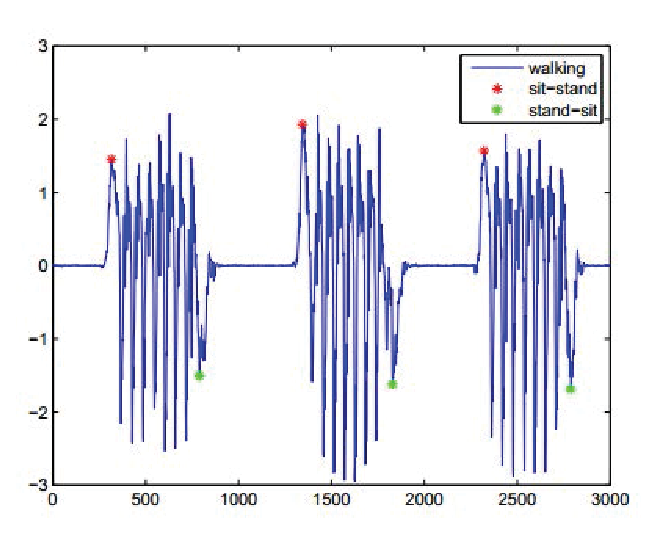
\includegraphics[width=0.45\textwidth]{transfer2.eps}}
    \caption{陀螺仪的时域信号}\label{transfer}
\end{figure}

从图中可以看出坐下和站起两个过渡状态与行走之间的差别。同时我们假定在所有行为中只有行走状态下才有可能在下一时刻转变为静止状态,基于此我们提出一种通过过渡状态的行为对静态行为进行分类识别的方法,其流程如图\ref{static_strategy}所示。

\begin{figure}[!htp]
\centering
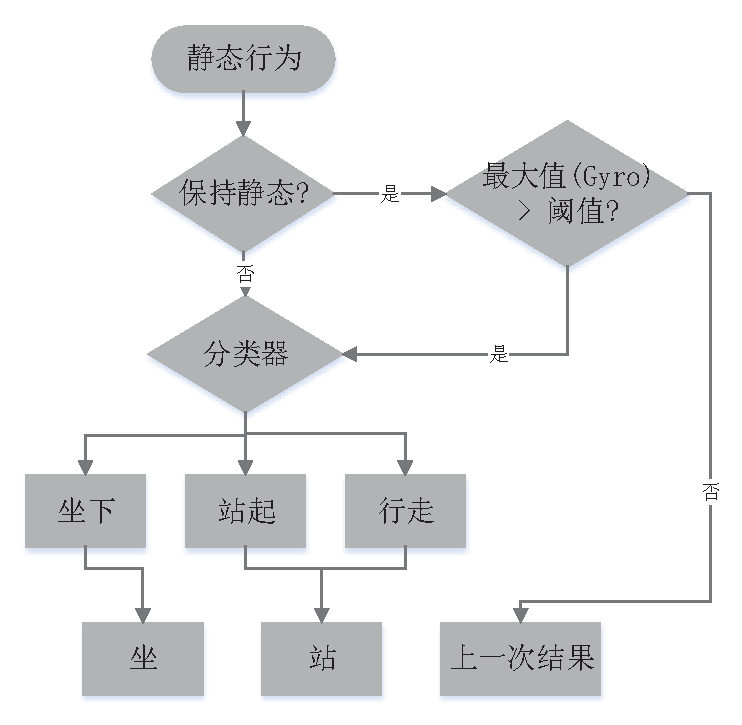
\includegraphics[width=0.6\textwidth]{static_strategy.eps}
\caption{静态行为分类策略流程图}\label{static_strategy}
\end{figure}

\par 如图\ref{static_strategy}所示,如果前一次第一层分类的识别结果为静态行为且陀螺仪关于角速度的信号模值的最值没有超过设定的阈值,则此次保持上次的判决结果。否则,对前一个判决周期内的过渡行为利用之前训练的分类器进行分类。根据这一分类器的分类结果,间接推断出静止的行为状态。

\subsection{动态行为分类策略}
\par 对于动态的行为,运动传感器所采集的数据很容易受到位置和方向变化的影响,因为当手机处于人体不同位置时,加速度等信息会表现出不同的信号模式\scite{lee2011activity}。因此分类器对动态行为的分类很容易受到手机所处位置和方向变化的影响,尤其是对于那些相似行为,即被分在同一组的行为。在本文中,我们提出一种位置辅助分类器的方法可以有效降低位置变化带来的影响。该方法的关键就是对于每一次判定为动态行为时,首先使用之前训练的位置分类器对其分类获取其位置信息。然后再针对不同位置,使用相应位置下所选取的最佳特征集以及所训练的分类器对其进行最终的行为分类。在本文中,在采集数据时智能手机分别被放置在四个不同位置,分别是手中,上衣口袋,裤子口袋,裤子背面口袋。在训练位置分类器时,上衣口袋被定义为上身位置,裤子口袋和裤子背部口袋被定义为下身位置。动态行为分类策略的过程如图\ref{dynamic_strategy}所示。
\begin{figure}[!htp]
 \centering
 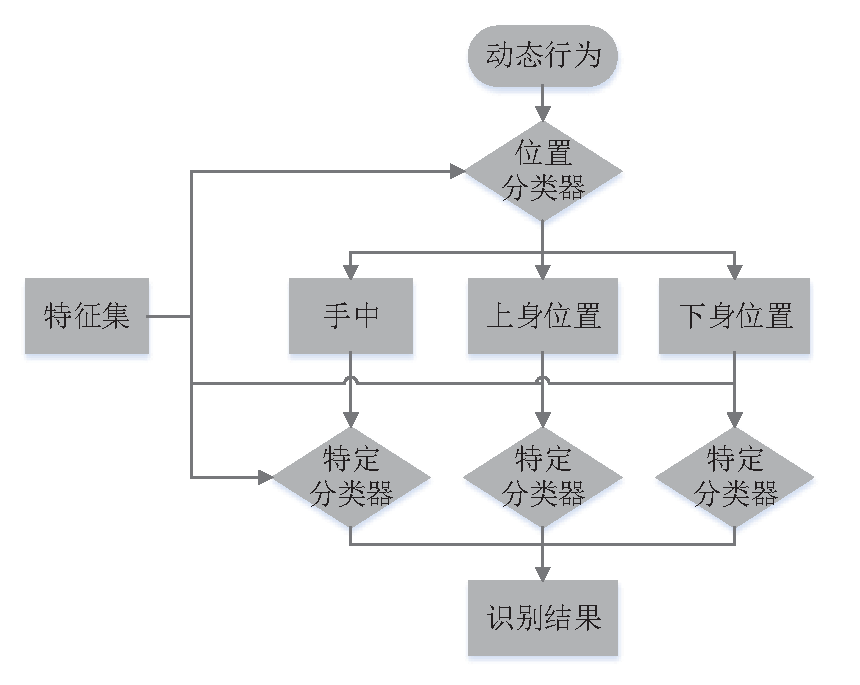
\includegraphics[width=0.8\textwidth]{dynamic_strategy.eps}
 \caption{动态行为分类策略}\label{dynamic_strategy}
\end{figure}
\par 引入位置辅助分类器不但可以有效降低位置变化带来的影响,而且还可以根据不同位置下运动传感器数据的不同特征选择各自最佳的特征集。针对于三类不同位置,本文利用信息增益作为特征的评价指标,对特征排序后各自选择最佳的前十个特征如图\ref{features}所示。从图中可以看出当智能手机手机处于手中时,更偏向于选择陀螺仪的时域和频域特征,对于上身口袋位置,选择加速度传感器和磁场传感器的特征对于分类更为有效,而当手机处于下身位置时,则更倾向于选择加速度传感器和陀螺仪的频域和相关函数有关的特征。因此,当智能手机处于不同位置时,选择各自最佳的特征集合进而训练各自最佳的分类器,可以有效改善最终的分类结果。
\begin{figure}[!htp]
 \centering
 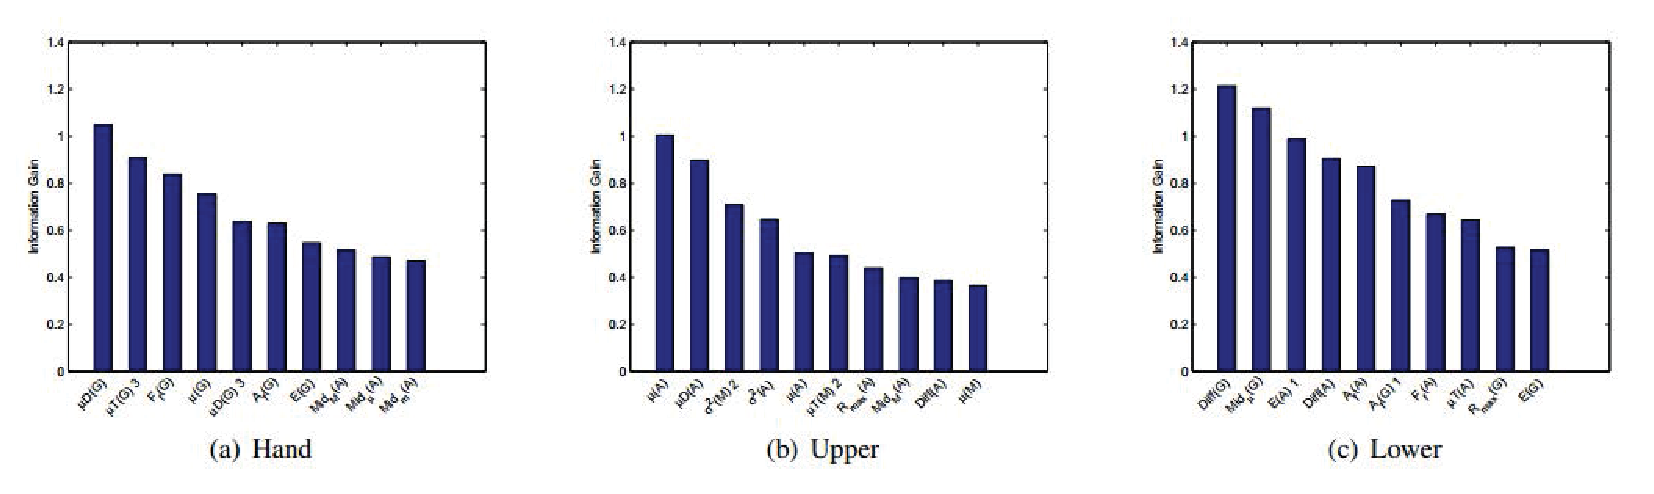
\includegraphics[width=1.0\textwidth]{features.eps}
 \caption{不同位置下各类特征的信息增益排序}\label{features}
\end{figure}

\section{分类实验结果}
\subsection{数据采集实验以及参数设定}
\par 在实验过程中,我们共有6人参与数据集的采集,而最初将所有传感器的采样率都设定为$50Hz$。我们所采集的数据集的时间分布如表格\ref{data_time}所示。所采集的数据会通过带有重叠的滑动窗口的机制对其进行分段,窗口的时间长度为$T=5s$,重叠率为50\%。对于每一个窗口内的数据可以提取我们前面所提到的一系列特征,然后每一个分类器都可以根据特征的信息增益选择最佳的特征集。在实验过程中,我们设定都选择信息增益最高的10个特征。

\begin{table}[!htbp]
\centering
\caption{实验数据的时间分配(单位:分钟$(min)$)}\label{data_time}
\begin{tabular}{|c|c|c|c|c|c|c|}
\hline
\diagbox{Position}{Time(minute)}{Activity} &ST &SD &WK &RN &AS &DS\\
\hline
Hand &12 &12 &30 &30 &30 &30\\
\hline
Coat Pocket &12 &12 &30 &30 &30 &30\\
\hline
Trouser Pocket &12 &12 &30 &30 &30 &30\\
\hline
Rear Pocket &0 &12 &30 &30 &30 &30\\
\hline
\end{tabular}
\end{table}

\par 对于分类器的选择,我们统一都是用随机森林作为默认的分类算法,该算法在\cite{bin2012classification}中,作者已经通过实验验证了其对行为识别的有效性。在计算每一层分类器的分类结果时,我们采用选择其中五个参与者的数据作为训练集,剩余一个参与者的数据作为测试集,然后依次执行六次,计算这六次的平均值。在本文中,结果的评定指标包括正例正确率(True Positive, TP),误报率(False Positiove, FP),准确率(Precision),召回率(Recall),F系数(F-Measure)\scite{brezmes2009activity}等。

\subsection{分类实验结果与分析}
\par 将所有行为分为三组以后,相应数据也合并为有三个类标签的数据,进而训练相应的随机森林分类器。在第一层使用该分类器对数据进行分组,其结果如表格\ref{first_level_result}所示。由于根据之前的分组原则,不同组之间行为的差异很大,所以第一层的识别效果比较好。
%第一层分类结果
    \begin{table}[!ht]
    \centering
    \caption{第一层分组分类的结果}\label{first_level_result}
    \begin{tabular}{cccccc}
    \toprule
    Classes & TP Rate & FP Rate & Precision & Recall & F-Measure \\
    \midrule
    Static & 0.997 & 0.001 & 0.997 & 0.997 & 0.997 \\
    Slow Dynamic & 0.997 & 0.004 & 0.997 & 0.997 & 0.997 \\
    Fast Dynamic & 0.993 & 0.001 & 0.992 & 0.993 & 0.993\\
    \hline
    Weighted Avg. & 0.997 & 0.003 & 0.997 & 0.997 & 0.997\\
    \bottomrule
    \end{tabular}
    \end{table}
%静态行为分类策略结果
\par 对于静态行为,本文仅以坐和站为例, 因此实验过程中采集了坐下、站起以及从静止变为行走等过渡状态下的数据。实验参与者周期性地进行坐下、站起、行走等,周期时间长度设定为15s。传感器数据被分段,时间窗口长度依然为$5s$,但是不再有重叠。然后从这些时间窗口内的数据中提取相应特征并利用训练数据训练随机森林分类器。最后使用该分类器对过渡行为进行分类,分类结果如表格\ref{static_result}所示。而通过过渡态的行为分类,根据我们之前所述的静态行为分类方法即可以间接获取静态的行为状态。

\begin{table}[!ht]
    \centering
    \caption{静态行为分类策略的分类结果}\label{static_result}
    \begin{tabular}{cccccc}
    \toprule
    Classes & TP Rate & FP Rate & Precision & Recall & F-Measure \\
    \midrule
    Sit-Stand & 0.9848 & 0.0014 & 0.9924 & 0.9848 & 0.9886\\
    Stand-Sit & 0.9924 & 0.0056 & 0.9704 & 0.9924 & 0.9813\\
    Walking & 0.9966 & 0 & 1.0000 & 0.9966 & 0.9983\\
    \hline
    Weighted Avg & 0.9941 & 0.0011 & 0.9942 & 0.9941 & 0.9941\\
    \bottomrule
    \end{tabular}
 \end{table}

 %动态行为分类策略结果
\par 在实验过程中,我们同样计算了位置分类器的分类准确率,这对于位置辅助的动态行为分类是十分重要的。如表格\ref{position_result}所示,位置分类器的分类准确率较高,因此首先进行的位置分类对于行为分类结果的准确率影响并不大,也就表明位置辅助的动态行为识别方法有其重要的意义。

%位置分类器的分类结果
 \begin{table}[!htb]
    \centering
    \caption{位置分类的分类结果}\label{position_result}
    \begin{tabular}{cccccc}
    \toprule
    Classes & TP Rate & FP Rate & Precision & Recall & F-Measure \\
    \midrule
    Hand & 0.9927 & 0.0033 & 0.9937 & 0.9927 & 0.9932\\
    Upper Body & 0.9282 & 0.0163 & 0.9058 & 0.9282 & 0.9169	\\
    Lower Body & 0.9720 & 0.0228 & 0.9782 & 0.9720 & 0.9751	\\
    \hline
    Weighted Avg & 0.9728 & 0.0152 & 0.9730 & 0.9728 & 0.9729\\
    \bottomrule
    \end{tabular}
 \end{table}

\par 最后,我们通过对本文提出的两层多策略的分类框架与之前两篇文献\cite{orientationTransation1},\cite{bisio2014comparison}所提出的方法做比较,对分类结果做出分析。为了与之前两篇文献的实验设定一直,本文的行为集中坐和站合并为一类,成为静止状态(SC)。最后的识别结果分别如表格\ref{final_result}, \ref{com_result1}, \ref{com_result2}所示。
%分类结果比较
 \begin{table}[htb]
    \centering
    \caption{本文框架的分类结果}\label{final_result}
    \begin{tabular}{cccccc}
    \toprule
    Classes & TP Rate & FP Rate & Precision & Recall & F-Measure \\
    \midrule
    SC & 0.9972 & 0.0010 & 0.9976 & 0.9972 & 0.9974 \\
    WK & \textbf{0.9974} & \textbf{0.0201} & \textbf{0.9384} & \textbf{0.9974} & \textbf{0.9575}	\\
    RN & 0.9938 & 0.0013 & 0.9925 & 0.9938 & 0.9934	\\
    AS & \textbf{0.8926} & \textbf{0.0193} & \textbf{0.8737} & \textbf{0.8926} & \textbf{0.8830} \\
    DS & \textbf{0.8654} & \textbf{0.0132} & \textbf{0.9312} & \textbf{0.8654} & \textbf{0.8971}	\\
    \hline
    Weighted Avg & \textbf{0.9570} & \textbf{0.0095} & \textbf{0.9571} & \textbf{0.9570} & \textbf{0.9567} \\
    \bottomrule
    \end{tabular}
 \end{table}

 \begin{table}[htb]
    \centering
    \caption{文献\cite{orientationTransation1}的分类结果}\label{com_result1}
    \begin{tabular}{cccccc}
    \toprule
    Classes & TP Rate & FP Rate & Precision & Recall & F-Measure \\
    \midrule
    SC & 0.9988 & 0 & 1.0000 & 0.9988 & 0.9994 \\
    WK & 0.8894 & 0.0245 & 0.9050 & 0.8894 & 0.8971	\\
    RN & 0.9935 & 0.0003 & 0.9978 & 0.9935 & 0.9957	\\
    AS & 0.7991 & 0.0541 & 0.7934 & 0.7991 & 0.7963 \\
    DS & 0.8517 & 0.0420 & 0.8395 & 0.8517 & 0.8456	\\
    \hline
    Weighted Avg & 0.9039 & 0.0249 & 0.9044 & 0.9039 & 0.9041 \\
    \bottomrule
    \end{tabular}
 \end{table}

  \begin{table}[htb]
    \centering
    \caption{文献\cite{bisio2014comparison}的分类结果}\label{com_result2}
    \begin{tabular}{cccccc}
    \toprule
    Classes & TP Rate & FP Rate & Precision & Recall & F-Measure \\
    \midrule
    SC & 0.9776 & 0.0012 & 0.9965 & 0.9776 & 0.9869 \\
    WK & 0.7714 & 0.0758 & 0.7319 & 0.7714 & 0.7511 \\
    RN & 0.9946 & 0.0011 & 0.9935 & 0.9946 & 0.9941 \\
    AS & 0.7456 & 0.0489 & 0.7894 & 0.7456 & 0.7669 \\
    DS & 0.7342 & 0.0659 & 0.7171 & 0.7342 & 0.7256 \\

    Weighted Avg & 0.8455 & 0.0384 & 0.8475 & 0.8455 & 0.8462 \\
    \bottomrule
    \end{tabular}
 \end{table}
\par 从表格中的对比数据中可以看出本文所提出的行为识别框架在一定程度上提高了识别准确率,尤其是对于慢速动态行为,如行走和上下楼等,其准确率具有较大幅度的提升。主要是由于在本文的框架中引入了位置分类器,可以根据运动特征判定位置,位置信息可以很好地指导进一步的行为分类。
 \section{本章小结}
 \par 本章主要介绍了我们所提出的基于智能手机的两层多策略的行为识别框架,该框架主要针对于解决基于智能手机的行为识别研究中主要存在的两个问题,即位置和方向变化的问题。首先本章介绍了数据获取以及特征提取的过程,重点讲述了本文提出的自相关函数的特征,该特征没有方向敏感性,可以在一定程度上降低方向变化的干扰。然后介绍了框架中的两层分类模型,即将所有行为根据相似度分成若干组,然后根据不同组行为的特点采样不同的分类策略作进一步分类。一方面,本文通过引入过渡状态行为辅助静态行为的分类,另一方面由于位置变化对动态行为分类识别的影响,本文通过引入位置分类器获取智能手机的位置信息,进而在特定位置下训练分类器对动态行为做进一步的分类。本章的最后给出了分类实验结果,并且与之前的研究工作做了对比实验,实验结果验证本文所提出框架在行为识别的性能上有了很大幅度的提升。

  \chapter{高能效的识别策略动态调整研究}
\par 在移动终端这个特殊的系统环境下,其中最大的限制就是能量有限。而在基于智能手机的行为识别整个过程中无论是内置传感器采集数据还是计算特征并对当前行为进行判决分类都会消耗较大的能量\scite{priyantha2010enabling}。因此我们有必要要研究在行为识别过程中降低手机能耗的方法,其最终目的就是通过权衡识别准确率和识别能耗,在保证一定准确率的前提下,尽可能降低在识别过程中智能手机的能耗。
\par 使用智能手机进行行为识别过程中,传感器采集运动数据,处理器计算特征向量以及运行分类算法对行为做判断识别都会消耗智能手机较多的能量。而在这一过程中,能耗的大小与传感器的采样率,采样时间,以及特征向量和分类算法的计算复杂度都有着直接的关系\scite{rachuri2011sociablesense}。另一方面,行为识别的识别准确率则取决于采集数据的充分性,特征集和分类算法的选择,所以准确率同样与采样率,采样时间,特征向量等的选择有直接关系\scite{ravi2005activity}。与此同时,不同的行为对数据量的要求,对特征集合的选择等都存在很大的不同\scite{raffa2010don},比如静止行为状态下,运动信息很少,对数据量的要求不高,而且也不存在频域特性,因此不需要在这段时间内以较高的采样率采集数据并计算频域等复杂特征,只需要运行较低的采样率监测过渡态行为是否发生即可。又比如在跑步状态下,其频域特征十分明显,且较容易识别,此时传感器只需要在窗口时间内的一部分时间采集数据就可以识别跑步状态,其他时间传感器进入休眠可以有效降低能耗。因此可以针对不同行为通过调节上述的一些变量,在较少影响准确率的情况下尽可能降低识别能耗。
\par 为研究高能效的识别策略调整方法,本章首先建立能耗和准确率的数学模型,研究二者与一些变量的函数关系,包括采样率,采样时间,特征集的选择等。与此同时,为了权衡识别准确率和识别能耗的关系,本文使用手机当前的能耗作为权衡系数,建立目标函数,为每一类行为求解识别策略只需要求解相应目标函数的最优值即可,即转换为最优化问题。然后通过实验测量数据求解数学模型参数,进而求解每类行为的目标函数的最优解,从而获得每一种行为的识别策略。最后提出一种结合行为识别结果和马尔科夫模型的行为转换矩阵的策略动态调整方法,最终达到高能效地进行行为识别的目的。

\section{数学模型}
\par 对于识别准确率和识别能耗的影响因素,本文考虑采样率,采样时间以及是否采用频域和自相关函数的特征作为变量研究准确率和能耗模型。本文中,采样率为传感器的数据采集速率,用$f$表示,采样时间使用窗口内的采样时间比例替代,如图\ref{window}所示,窗口时间长度为$T$,相邻窗口有50\%的重叠,其中有一定比例的窗口时间用于采集数据,比例用$\tau$表示。而是否使用频域和自相关函数的特征则可以使用0或1的离散变量表示,本文对其分为四种情况分别讨论。下面将讨论如何建立能耗与准确率模型,以及如何构建目标函数,进而为每类行为求解识别策略。

\begin{figure}[ht]
\centering
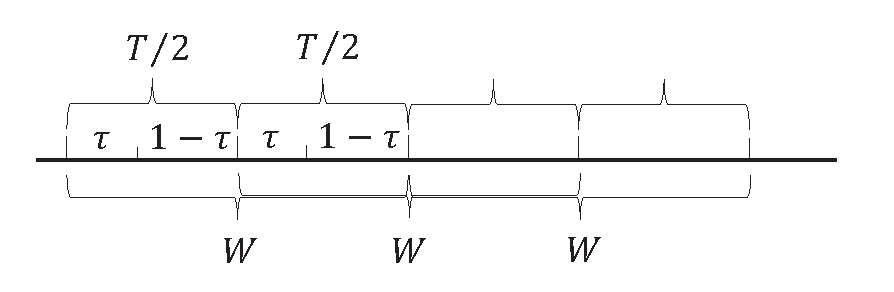
\includegraphics[width=8cm]{window.eps}
\caption{时间窗口示意图}\label{window}
\end{figure}

\subsection{能耗模型}
\par 使用智能手机执行行为识别过程中,能量损耗主要包括传感器的数据采集能耗和处理器的计算能耗两部分,因此能耗模型可以表示为:
\begin{equation}
	E(t) = E_S(t) + E_M(t)
\end{equation}
\par 首先是数据采集能耗,由于传感器是集成在智能手机内部,通常是由处理器负责充当传感器采集数据的ADC模块,传感器只负责运行采集模拟信号,处理器则根据指定的采样率采集离散信号,此外由处理器负责开启和关闭传感器。因此,数据采集能耗主要包括传感器运行能耗,处理器采集数据能耗以及传感器工作与休眠状态切换能耗。数据采集能耗的模型可以表示为:
\begin{equation}
	E_S(t) = (P_S\tau + P_A(f)\tau + P_{on-off}) \times t
\end{equation}
其中,$P_S$为传感器功率,$P_A$为处理器作为ADC模块采集数据时的功率,该功率与采样率有关,$P_{on-off}$为一定时间内处理器控制传感器切换工作和休眠状态时的等效平均功率,可以通过一段时间以确定频率周期性切换状态时能耗除以时间长度计算得到。
\par 其次是数据处理与计算能耗。行为识别过程中的数据处理和计算主要包括计算特征向量和运行分类算法。由于本文中,特征集包括时域、频域和自相关函数特征三个方面,而时域特征可以通过时域信号直接计算,计算量较小,能耗较低,因此本文方案总是使用时域特征,不再将其作为一个变量。与此同时,频域和自相关函数的特征需要对信号做快速傅里叶变换和求解自相关函数,计算量较大,因此本文将是否使用这两个类型的特征作为两个离散变量考虑进能耗模型中,而根据频域信号和自相关函数计算相应特征则过程十分简单,能耗相对较小,本文中将其忽略。因此数据处理能耗可以表示为:
\begin{equation}
	E_M(t) = (\mu E_{FFT} + \lambda E_{ACF} + E_C) \times \theta \times t
\end{equation}
其中,$E_{FFT}$和$E_{ACF}$分别表示计算单次FFT和ACF所消耗的能量,$\mu$,$\lambda$取值为0或1,表示不使用或使用频域或自相关函数的特征,$E_C$表示运行分类算法对行为实例分类时的能耗。$\theta$表示单位时间内执行识别分类的次数,因为在一个时间窗口内执行一次识别,需要计算一次FFT和ACF,用于提取频域和自相关函数的特征,因此数据处理的等效平均功率即可以表示单次执行分类的所有能耗乘以单位时间内执行分类的次数。

\subsection{准确率模型}
\par 行为识别的准确率同样也是主要受到来自本文所提到的四个变量的影响,即采样率,采样时间比例,是否采用频域和自相关函数的特征。对于采样率和采样时间比例,二者均为连续变量,本文重点研究准确率与二者的函数关系,而对于是否使用频域和自相关函数的特征则是两个离散值,因此在本文中分成四种不同情况讨论准确率模型。下面以使用全部特征,即包含频域和自相关函数特征为例说明准确率模型,其他三种情况与之类似。
\par 首先识别准确率是受到采样率和采样时间的影响,但是它与二者没有确定的显式函数关系,其次不同行为的识别准确率对采样率和采样时间的敏感程度也会有所不同\scite{wang2009framework},比如对于静止状态的行为,由于其运动传感器的数据在一定时间内变化不大,采样率的大小对其影响较小,而对于快速运动状态,其识别准确率则很大程度地依赖采样率的大小。所以本文首先建立识别准确率与采样率和采样时间比例的数学模型,然后针对每一类行为通过实验训练集数据的识别结果拟合数学模型参数,从而获得最适合该行为的函数关系模型。

\begin{figure}[!htb]
    \centering
    \subfloat[行走状态下的识别准确率]{
    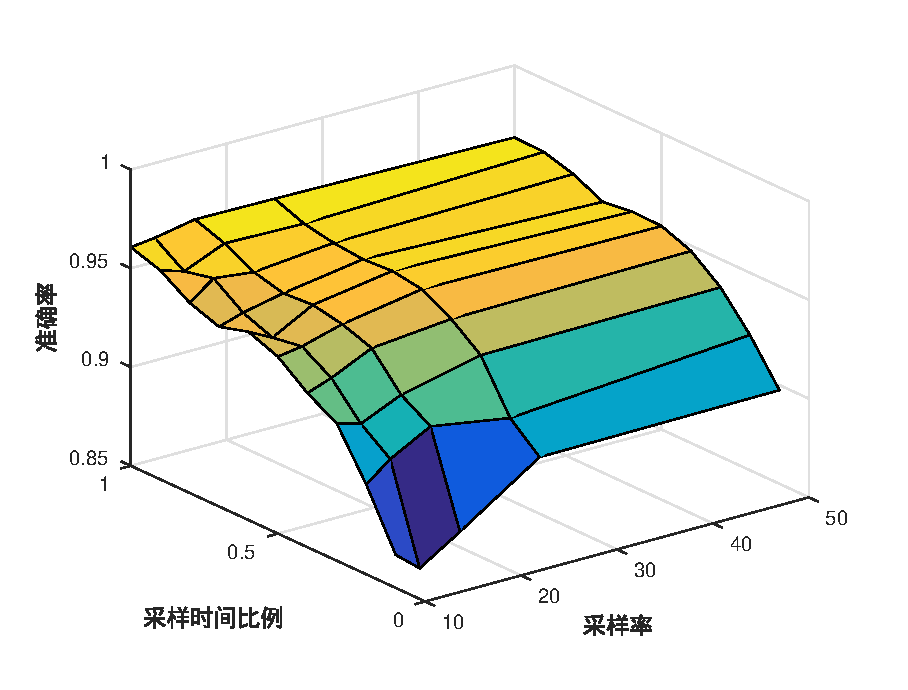
\includegraphics[width=0.45\textwidth]{walk_precision.eps}}
    \subfloat[跑步状态下的识别准确率]{
    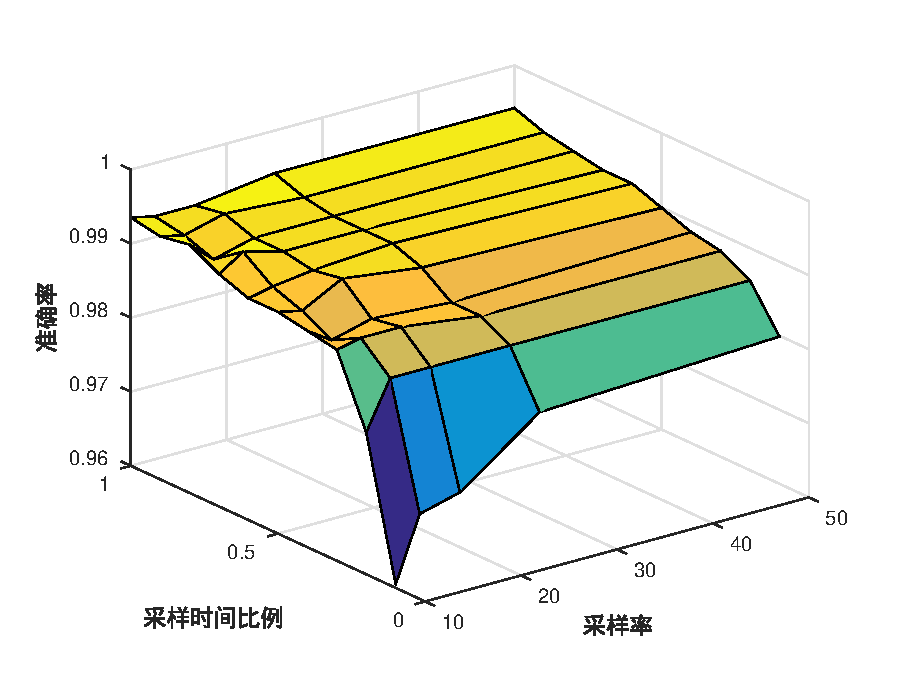
\includegraphics[width=0.45\textwidth]{run_precision.eps}}
    \caption{识别准确率与采样率和采样时间比例的关系}\label{precision}
\end{figure}

\par 图\ref{precision}(a)和\ref{precision}(b)分别表示行走状态和跑步状态下,实验训练集数据识别准确率与采样率和采样时间比例的关系。从图中我们可以看出准确率与两个变量之间基本都是成负指数函数关系。因此本文考虑为识别准确率建立以下数学模型:
\begin{equation}
	Precision(i) = exp(-\frac{\alpha_i}{f} - \frac{\beta_i}{\tau})
\end{equation}
其中,$\alpha_i$,$\beta_i$为待拟合参数,$f$表示采样率,$\tau$表示采样时间比例,$i$表示某一类行为$i$。
\par 在建立识别准确率的数学模型以后,根据不同采样率和采样时间比例的训练集数据即可拟合该数学模型,从而获得相应的模型参数。
\subsection{目标函数}
\par 本部分研究的根本目标是为行为识别选择一种识别策略,使得在保证一定准确率的前提下,尽可能降低在识别过程中的各部分能量损耗。但是识别准确率和能耗存在明显的矛盾关系,因此选择识别策略需要在能耗与准确率之间寻找一个最佳的权衡。为了更好地考虑和权衡二者的关系,本文通过建立目标函数将准确率和能耗统一在一个目标函数中。
\par 建立目标函数首先需要考虑的是权衡系数问题,即能耗和准确率不同的重要程度。本文考虑将智能手机的电量离散化为若干等级,并使用当前电量所处的等级所谓权衡系数,当电量充足时提升准确率在目标函数的重要程度,电量较少时则提升能耗在目标函数中的重要程度。其次是准确率和能耗的数值归一化问题。准确率是一个比例,其数值大部分分布在0.8到1.0之间,而能耗的数值则是一个实数,为执行一次行为识别的耗电量,为了更好权衡二者关系需要将其数值做归一化处理。本文考虑为准确率设定可接受的准确率最低阈值$Precision_{low}$,并将准确率从$Precision_{low}$到1.0的数值映射到0到1.0之间,对于准确率低于阈值的情况则变换为负无穷,即不可接受的准确率。对于能耗的归一化,本文考虑通过将能耗数值除以“最强策略”的能耗值做归一化。所谓“最强策略”即使用可设定的最高采样率,100\%的采样时间比例以及使用频域和自相关函数的特征情况。最后是离散变量问题,即是否使用频域和自相函数特征是两个独立且离散的变量,直接将其放入目标函数会对求解最优化问题造成困难,因此在构建目标函数时,本文同之前的考虑相同,将其作为四种情况分类讨论,在求解最优化问题时,从四个求解得到的最优目标函数值中再择最优即可。
\par 确定目标函数以后,为每类行为选择识别策略就可以转换为求解目标函数最优值的最优化问题,而优化变量即为待求解的识别策略。其中最优化问题可以表示为:
\begin{equation}
  \begin{array}{ll}
    \min \limits_{f, \tau, \mu, \lambda}  & z=\{(1-\varphi (battery)) \frac{E_T}{E_{max}} - \varphi (battery) \frac{Precision(i) - Precision_{low}}{1 - Precision_{low}}\} \\
    \\
    s.t. & \begin{array}[t]{rll}
             \mu 			 &  =    & 0|1 \\
             \lambda         &  =    & 0|1  \\
             Precision(i)    & \geq  & Precision_{low}
           \end{array}
  \end{array}
\end{equation}

其中,$E_{max}$表示“最强策略”下的能耗,$Precision_{low}$表示准确率的最低阈值,也是可以接受的最低识别准确率。$\mu, \lambda$表示是否使用频域和自相关函数特征,此最优化问题根据$\mu, \lambda = 0|1$分为四类情况分别求解,然后在其中取最优值。该最优化问题的解中对应的优化变量,即$f$, $\tau$, $\mu$和$\lambda$为对应行为的识别策略。


\section{模型求解}
\par 通过上一小节建立的数学模型以及目标函数,本文是通过求解一个关于目标函数的最优化问题为每类行为计算其对应的识别策略。本小节将详细介绍上述各数学模型参数的具体求解过程。首先是对于能耗模型,本文通过开发手机应用,在一系列的固定时间段内采用设定的采样率采集数据,以及一系列固定次数的特征计算,然后通过线性拟合的方式求解能耗模型的各个参数。其次对于准确率模型,本文将之前采集的数据做下采样或截断处理,使其满足一系列指定采样率和采样时间比例,然后通过对其分类求取的准确率对建立的准确率数学模型做曲面拟合,求取模型中的参数值。最后在获得具体模型以后,即可以通过求解目标函数最优值为每一类行为获取识别策略。

\subsection{能耗模型求解}
\par 能耗模型的求解需要实际测量智能手机在采集数据和计算特征等时所消耗的能量。为此,本文以Android操作系统为例,编写手机应用,执行数据采集或者数据处理等逻辑,进而测量该过程中的能量损耗。在手机应用中数据采集或数据处理能耗主要以耗电量的形式表示,而为了更为精确地测量应用的耗电量,Android系统提供了dumpsys工具可以用于查看系统服务信息和状态,通过该工具的battery命令即可以查看某应用一段时间内的耗电量。battery命令可以给出手机上每个进程的各个硬件的详细耗电量,包括处理器,WiFi和传感器等,因此本文使用它可以很精确测量数据采集和数据处理的各部分能耗。
\par 首先需要明确能耗测量实验设定,本文使用Google的Nexus5智能手机运行能耗测量应用,该应用可设定数据采样率,采样时间比例以及计算快速傅里叶变换或自相关函数的次数,并测量相应的手机耗电量,单位是mAh。其次是在数据采集部分,本文设定采样率为15Hz, 25Hz, 40Hz, 50Hz, 100Hz;采样时间比例设定为100\%,50\%,0\%。由于传感器运行能耗可以单独测量,但是处理器能耗则包括数据采集,控制传感器工作状态切换以及其他控制逻辑的多方面的能耗,无法单独测量,因此本文中首先设定100\%的采样时间比例可以使得在没有处理器控制传感器切换传感器工作状态时干扰的情况下研究不同采样率的数据采样能耗与采样率的关系,然后设置50\%的采样时间比例所测得结果,通过减去对应一半时间用于数据采样的能耗就可以得到处理器控制传感器切换工作状态的能耗,最后设置0\%的采样时间比例是为了测量其他控制逻辑的能耗,使得在计算各部分能耗时减去该部分能耗。测量实验在不同的采样率和采样时间比例的情况下,设定测量时间为1到5分钟,五个时间段,分别统计应用中传感器和处理器的能耗,每一组实验设定情况下重复测量5次,求取平均值作为该实验设定实验参数下的能耗结果,最后通过拟合能耗与时间的关系计算各部分的耗能功率。

	(1) 传感器功率
\par 传感器作为智能手机内置硬件,其能耗可以单独测量,因此计算较为简单。表格\ref{100_energy}和\ref{50_energy}为实验测量得到的传感器能耗。

\begin{table}[htb]
    \centering
    \caption{100\%采样时间情况下传感器能耗(单位:毫安时$(mAh)$)}\label{100_energy}
    \begin{tabular}{cccccc}
    \toprule
     $T(min)$ & 1 & 2 & 3 & 4 & 5 \\
    \midrule
    15Hz & 0.00321 & 0.00655 & 0.0099 & 0.0132 & 0.0166 \\
    25Hz & 0.00319 & 0.00655 & 0.00988 & 0.0132 & 0.0166 \\
    40Hz & 0.00321 & 0.00651 & 0.0197 & 0.0132 & 0.0166 \\
    50Hz & 0.00325 & 0.00654 & 0.0197 & 0.0132 & 0.0166 \\
    100Hz & 0.0032 & 0.00659 & 0.0099 & 0.0132 & 0.0164 \\
    \bottomrule
    \end{tabular}
 \end{table}

 \begin{table}[htb]
    \centering
    \caption{50\%采样时间情况下传感器能耗(单位:毫安时$(mAh)$)}\label{50_energy}
    \begin{tabular}{cccccc}
    \toprule
     $T(min)$ & 1 & 2 & 3 & 4 & 5 \\
    \midrule
    15Hz & 0.00159 & 0.00324 & 0.00491 & 0.00641 & 0.0081 \\
    25Hz & 0.00159 & 0.00327 & 0.00485 & 0.0067 & 0.00823 \\
    40Hz & 0.00158 & 0.00318 & 0.00483 & 0.00644 & 0.00815 \\
    50Hz & 0.0016 & 0.00322 & 0.0049 & 0.00641 & 0.00815 \\
    100Hz & 0.00159 & 0.00325 & 0.00482 & 0.00656 & 0.008 \\
    \bottomrule
    \end{tabular}
 \end{table}


\par 从数据中可以明显看出传感器的能耗与采样率无关,与时间成正比。因为与采样率无关,这里以50Hz采样率情况下的数据为例,进行线性拟合后如图\ref{sensor_energy}所示,可以发现明显的正比关系。通过线性拟合求取斜率可以计算出传感器的功率为$P_S = 3.4 \times 10^{-3} (mAh/min)$。

\begin{figure}[htb]
\centering
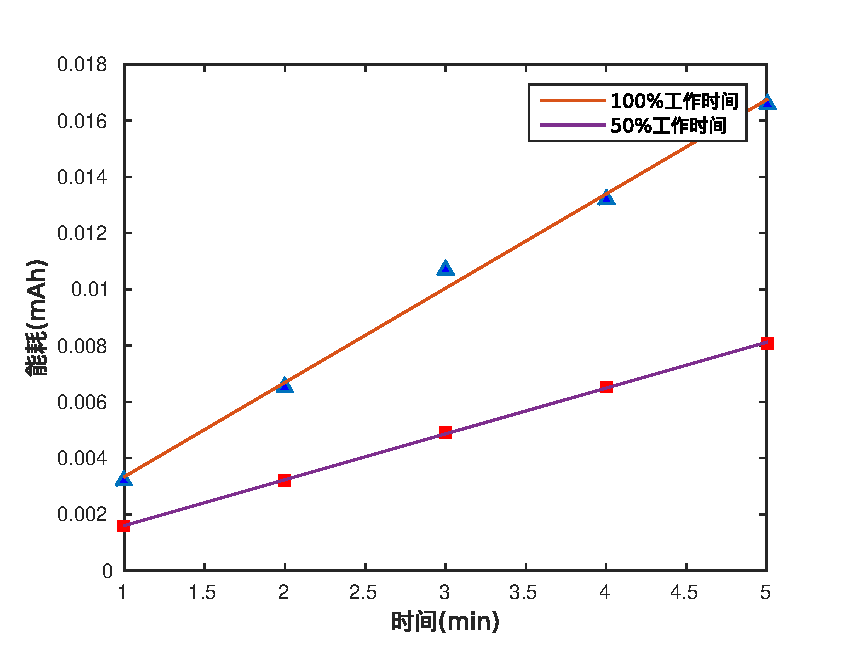
\includegraphics[width=0.5\textwidth]{sensor_energy.eps}
\caption{50Hz的采样率情况下传感器能耗与时间的关系}\label{sensor_energy}
\end{figure}

\begin{figure}[!htb]
    \centering
    \subfloat[15Hz采样率]{
    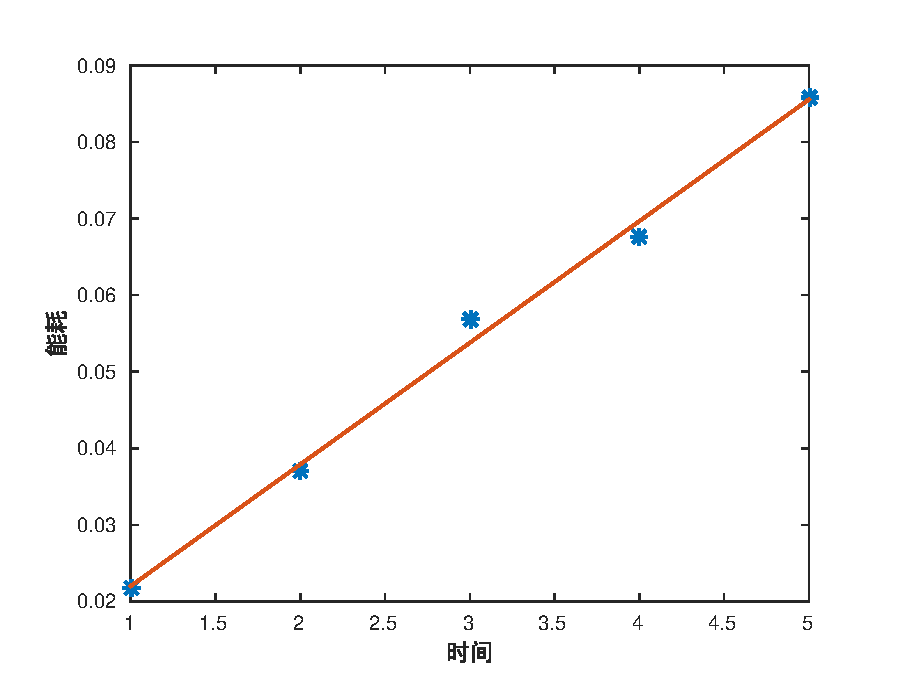
\includegraphics[width=0.3\textwidth]{100_sample_15Hz.eps}}
    \subfloat[]{
    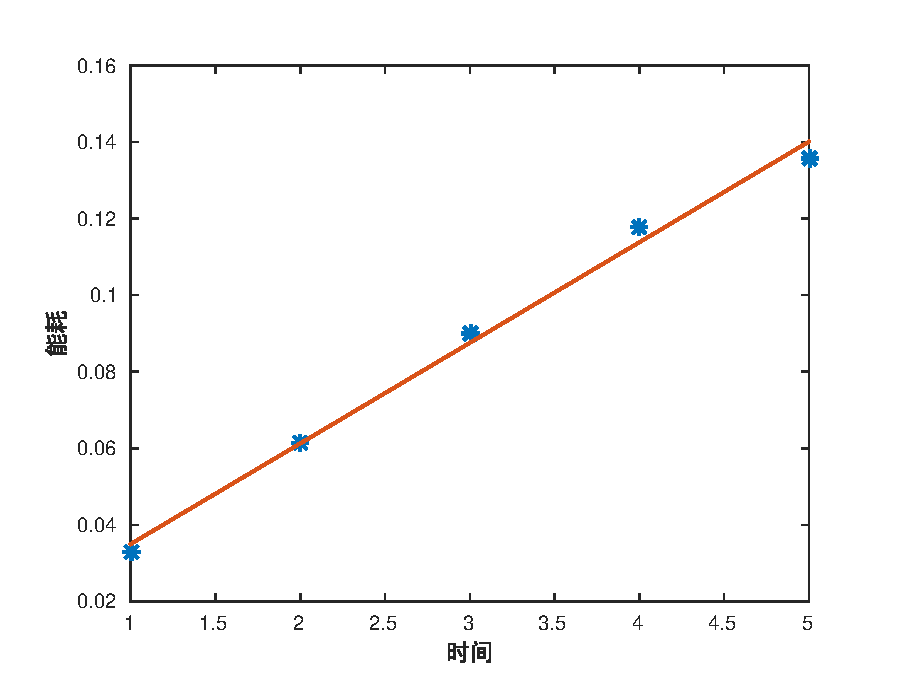
\includegraphics[width=0.3\textwidth]{100_sample_25Hz.eps}}
    \subfloat[40Hz采样率]{
    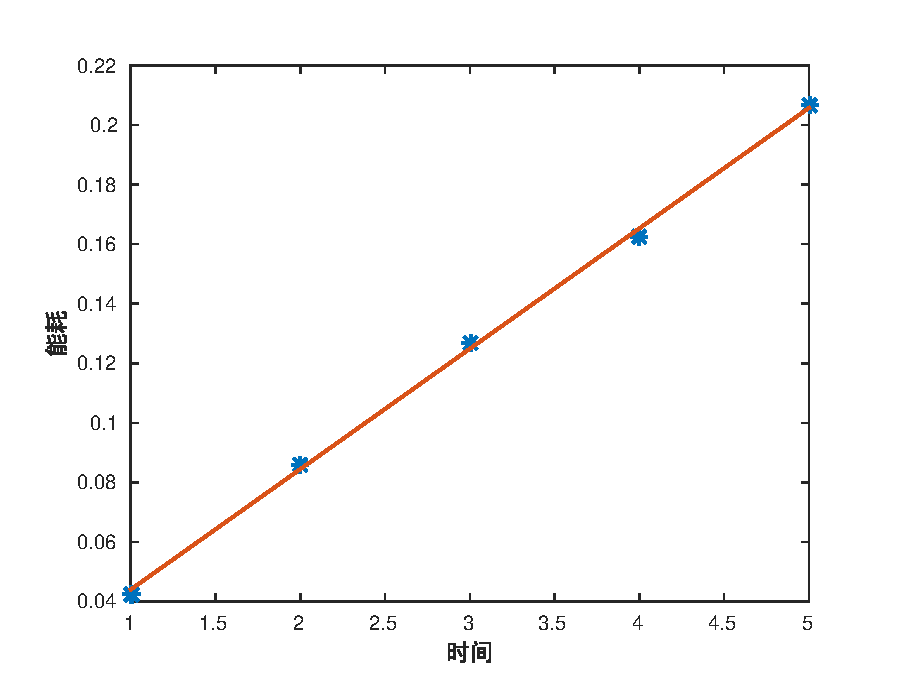
\includegraphics[width=0.3\textwidth]{100_sample_40Hz.eps}}
\caption{100\%采样时间以及各采样率情况下处理器的数据采集能耗与时间的关系(1)}\label{sample1}
\end{figure}
\begin{figure}[htb]
    \centering
    \subfloat[50Hz采样率]{
    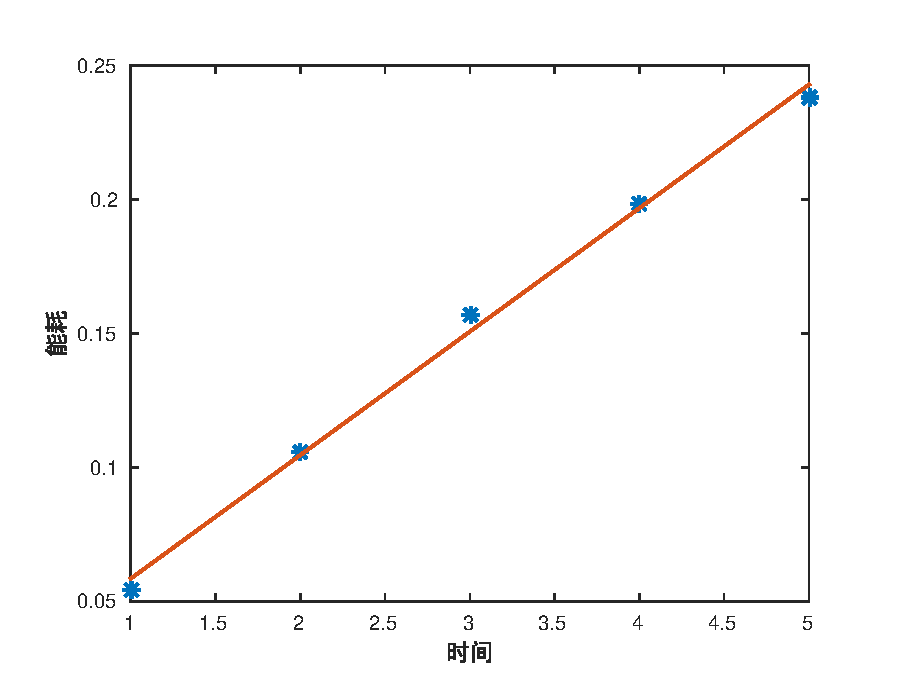
\includegraphics[width=0.3\textwidth]{100_sample_50Hz.eps}}
    \subfloat[100Hz采样率]{
    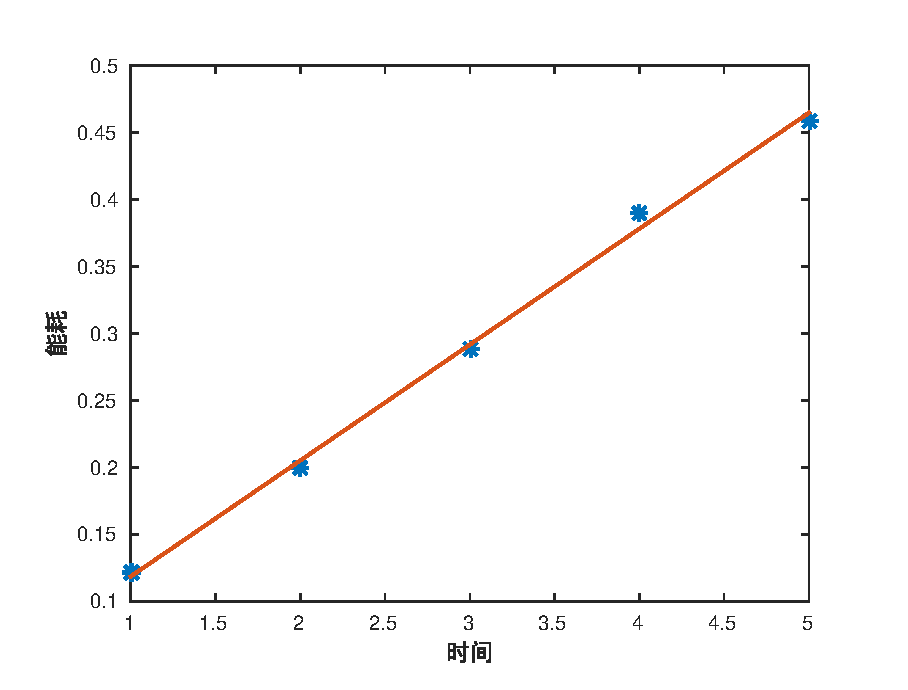
\includegraphics[width=0.3\textwidth]{100_sample_100Hz.eps}}
    \caption{100\%采样时间以及各采样率情况下处理器的数据采集能耗与时间的关系(2)}\label{sample2}
\end{figure}

	(2) 处理器的数据采集功率
\par 在智能手机内部由处理器充当传感器ADC模块的角色,负责数据采集。本文首先设定100\%的数据采样时间比例,即持续采集数据,避免了处理器在控制传感器切换状态时带来的能耗方面的干扰。然后在5个采样率的实验设定情况下,测量5种时间段内处理器的数据采集能耗,多次测量结果的平均能耗最为该实验设定的结果,研究与时间的关系如图\ref{sample1}(a)-(c)和\ref{sample2}(a)-(b)所示。
\par 从图\ref{sample1}和\ref{sample2}中可以看出,在每个采样率的情况下平均能耗都与时间成正比,即数据采集功率是保持恒定的。因此本文通过线性拟合可以计算得到每个采样率情况下的数据采集功率,而数据采集功率与采样率的关系如图\ref{p_sample_rate}所示。从图可以看出,数据采集功率同样与采样率也是成正比,经过线性拟合,可以计算得到功率与采样率的关系,其正比系数为$\alpha = 8.3962 \times 10^{-4} \quad mAh/min*Hz$。

\begin{figure}[htb]
\centering
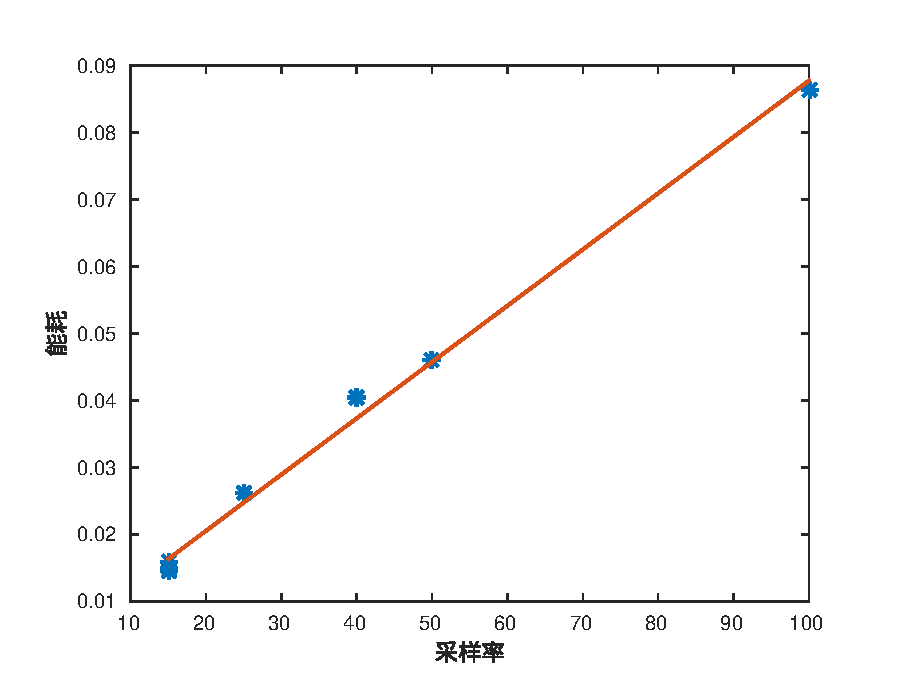
\includegraphics[width=0.5\textwidth]{p_sample_rate.eps}
\caption{处理器数据采集功率与采样率的关系}\label{p_sample_rate}
\end{figure}

	(3) 处理器的控制状态切换等效平均功率
\begin{figure}[htb]
    \centering
    \subfloat[50\%的时间比例情况下采集数据时处理器的能耗]{
    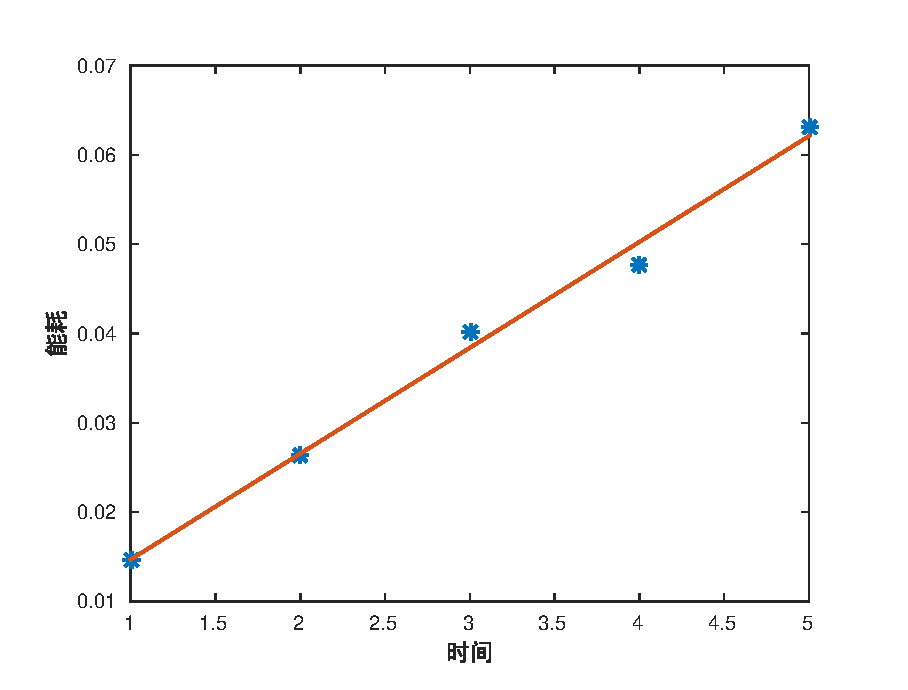
\includegraphics[width=0.45\textwidth]{50_sample_15Hz.eps}}
    \subfloat[处理器控制传感器状态切换时的能耗]{
    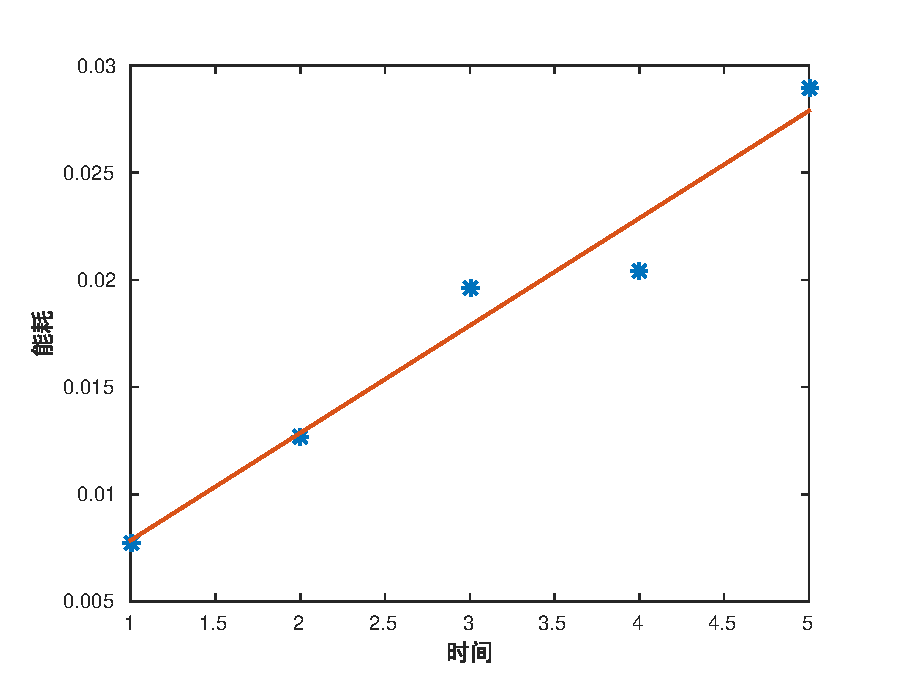
\includegraphics[width=0.45\textwidth]{on-off_p.eps}}
    \caption{处理器能耗与时间的关系}\label{on-off}
\end{figure}

\par 由于处理器的多任务性,无法单独测量控制状态切换功率,因此本文设定50\%的采样时间比例以及15Hz测量处理器能耗,并且设定没2.5s传感器状态切换一次,即一个开关的周期,该时间与行为识别中执行一次识别判定的时间相同。如图\ref{on-off}(a)所示为50\%的时间比例情况下采集数据时处理器的能耗与时间的关系。通过从中减去50\%的时间内数据采集的能耗(该能耗可以通过该采样率下的数据采集功率乘以数据采集时间计算得到)即可以获得控制传感器工作状态切换能耗。在15Hz的采样率下,控制状态切换的能耗与时间的关系如图\ref{on-off}(b)所示。此外,在其他采样率下可以通过相同方法计算处理器控制传感器状态切换能耗,其结果在误差范围以内与之相同。从\ref{on-off}(b)图中可以看出,该能耗与时间正比,虽然在每次发生状态切换时才会有能耗,但是通过线性拟合可以计算其等效平均功率,这也有助于能耗模型的计算。最后控制状态切换等效平均功率为:$P_{on-off} = 3.6 \times 10^{-3} (mAh/min)$。在当前实验设定情况下,每分钟传感器的状态切换24次,因此每次切换的能耗为$E_{on-off} = 1.5 \times 10^{-3}(mAh)$

	(4) 处理器的数据处理等效平均功率

\par 由于本文只考虑是否使用频域或自相关函数特征作为调节变量,因此只测量处理器在计算快速傅里变换(FFT)和自相关函数(ACF)的能耗,而特征计算与之相比数值较小,可以忽略不计。本实验通过设定一系列的执行次数测量处理器能耗,其结果如表格\ref{compute_energy}所示。图\ref{fft_acf}表示处理器计算FFT和ACF的能耗与执行次数的关系,从中也可以看出明显正比关系。

\begin{table}[htb]
    \centering
    \caption{处理器计算FFT和ACF的能耗(单位:毫安时$(mAh)$)}\label{compute_energy}
    \begin{tabular}{ccccccccccc}
    \toprule
    执行次数 & 1000 & 2000 & 3000 & 4000 & 5000 & 6000 & 7000 & 8000 & 9000 & 10000 \\
    \midrule
    FFT & 0.111 & 0.335 & 0.640 & 0.743 & 1.043 & 1.42 & 1.56 & 1.72 & 1.97 & 2.715 \\
    ACF & 0.084 & 0.152 & 0.226 & 0.299 & 0.362 & 0.408 & 0.569 & 0.596 & 0.809 & 0.883 \\
    \bottomrule
    \end{tabular}
 \end{table}

\begin{figure}[htb]
\centering
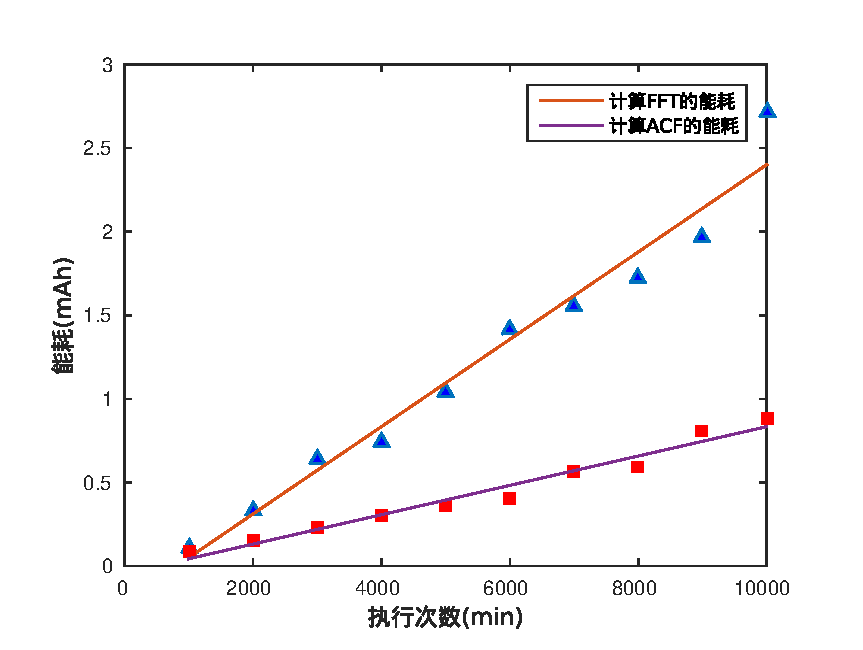
\includegraphics[width=0.5\textwidth]{fft_acf.eps}
\caption{处理器计算FFT和ACF的能耗与执行次数的关系}\label{fft_acf}
\end{figure}

通过线性拟合,可以得到单次计算傅里叶变换和自相关函数的能耗分别为$E_{FFT} = 0.30 \times 10^{-3} mAh, E_{FFT} = 0.10 \times 10^{-3} mAh$。为了便于计算,本文使用同一计量单位,为此分别计算其等效平均功率,即乘以单位时间内执行计算次数 $\theta = 24$, 即2.5s执行一次计算,与之前的进行一次识别判定相同, 其等效平均功率为:$P_{FFT} = 7.20 \times 10^{-3} mAh/min, E_{FFT} = 2.40 \times 10^{-3} mAh/min$。

\subsection{准确率模型求解}
\par 首先是实验设定,本文使用之前采集的50Hz采样率,100\%时间采样的情况下所获取的训练数据集。实验设定5Hz, 10Hz, 16.7Hz, 25Hz, 50Hz五个采样率,10\%到100\%十个采样时间比例。然后对原始训练数据集进行下采样和数据窗口内截断等方法获取实验设定中采样率和采样时间各个组合设定条件下的数据集。最后针对每个数据集,根据是否使用频域和自相关函数特征分为四组,分别提取规定特征并进行分类实验,最终获取分类的准确率结果。

\begin{figure}[htb]
    \centering
    \subfloat[实际的行走识别准确率]{
    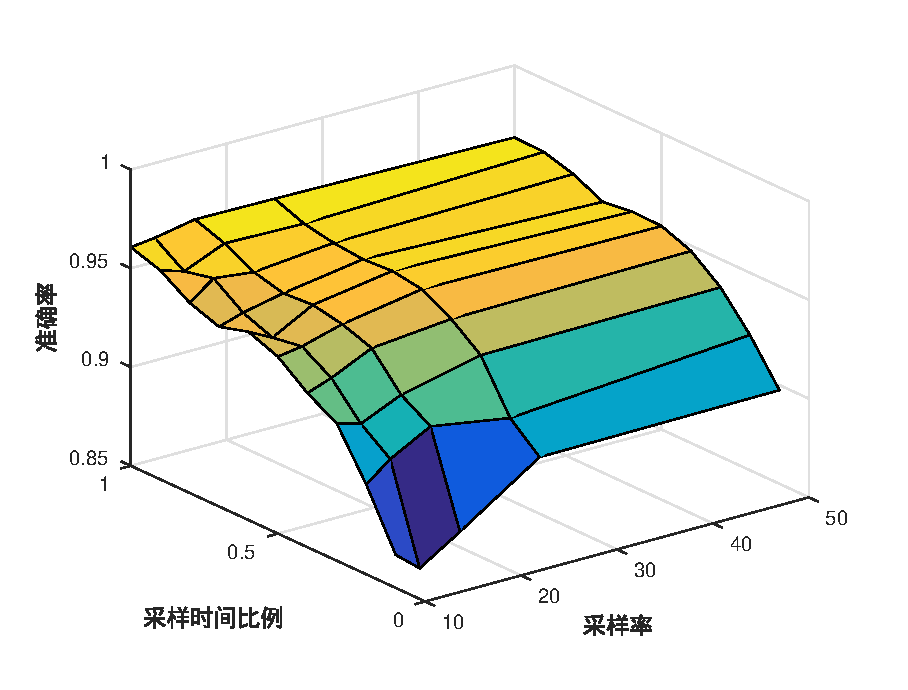
\includegraphics[width=0.45\textwidth]{walk_precision.eps}}
    \subfloat[拟合的行走识别准确率]{
    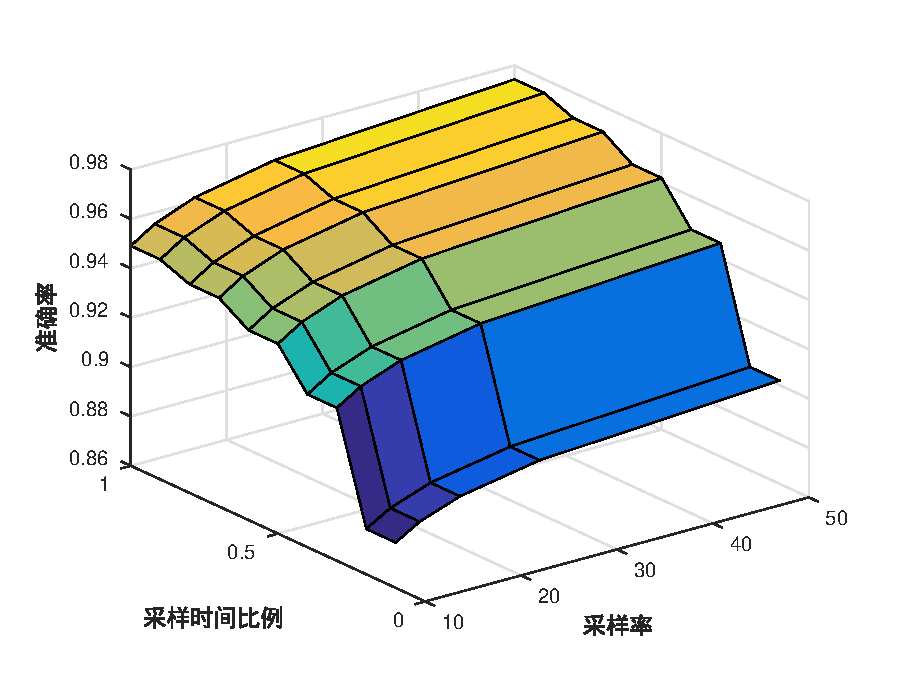
\includegraphics[width=0.45\textwidth]{walk_precision_fit.eps}}
    \caption{行走状态下的识别准确率与采样率以及采样时间比例之间的关系}\label{fit_precision}
\end{figure}

\par 图\ref{fit_precision}(a)为在使用频域和自相关函数特征的情况下,行走准确率与采样率和采样时间比例的关系,本文考虑使用曲面拟合的方法求解准确率模型中的参数。拟合后的效果如图\ref{fit_precision}(b)所示,从图中可以看出拟合后的曲面可以较好地反映出准确率与两个变量的函数关系。同样地,对于其他行为在不同的特征选择范围情况下也可以通过曲面拟合并求解参数,最后求解的参数和拟合残差结果如表格\ref{fit_result}所示。

\begin{table}[htb]
    \centering
    \caption{处理器计算FFT和ACF的能耗(单位:毫安时$(mAh)$)}\label{fit_result}
    \begin{tabular}{ccccccc}
    \toprule
    特征选择范围 &  参数 & 静止 & 行走 & 跑步 & 上楼 & 下楼\\
    \midrule
    \multirow{3}{2cm}{使用全部特征} & $\alpha$ & 0.112725 & 0.328838 & 0.041147 & 0.142354 & 0.10464 \\
    & $\beta$ & 0.001404 & 0.009677 & 0.001975 & 0.022183 & 0.029299 \\
    & 残差 & 0.000536 & 0.005263 & 0.000677 & 0.031337 & 0.078689 \\
    \midrule
    \multirow{3}{2cm}{使用时域和频域特征} & $\alpha$ & 0.125692 & 0.344354 & 0.041036 & 0.185501 & 0.04843 \\
    & $\beta$ & 0.001725 & 0.009621 & 0.002006 & 0.021795 & 0.029252 \\
    & 残差 & 0.000667 & 0.004364 & 0.000897 & 0.032815 & 0.06864 \\
    \midrule
    \multirow{3}{2cm}{使用时域和频域特征} & $\alpha$ & 0.099123 & 0.376837 & 0.056402 & 0.369427 & 0.128952 \\
    & $\beta$ & 0.001372 & 0.010081 & 0.001988 & 0.022509 & 0.029771 \\
    & 残差 & 0.000405 & 0.006223 & 0.000679 & 0.02864 & 0.057017 \\
    \midrule
    \multirow{3}{2cm}{仅使用时域特征}  & $\alpha$ & 0.116857 & 0.520193 & 0.067148 & 0.593838 & 0.616581 \\
    & $\beta$ & 0.001653 & 0.010415 & 0.c001989 & 0.021963 & 0.029101 \\
    & 残差 & 0.000669 & 0.009035 & 0.000756 & 0.029607 & 0.041895 \\
    \bottomrule
    \end{tabular}
\end{table}
\par 从表格\ref{fit_result}中可以看出拟合残差都较小,基本上都在5\%以内,这说明本文的准确率数学模型可以很好地刻画准确率与采样率和采样时间比例之间的关系。

\begin{figure}[htb]
    \centering
    \subfloat[静止状态的目标函数]{
    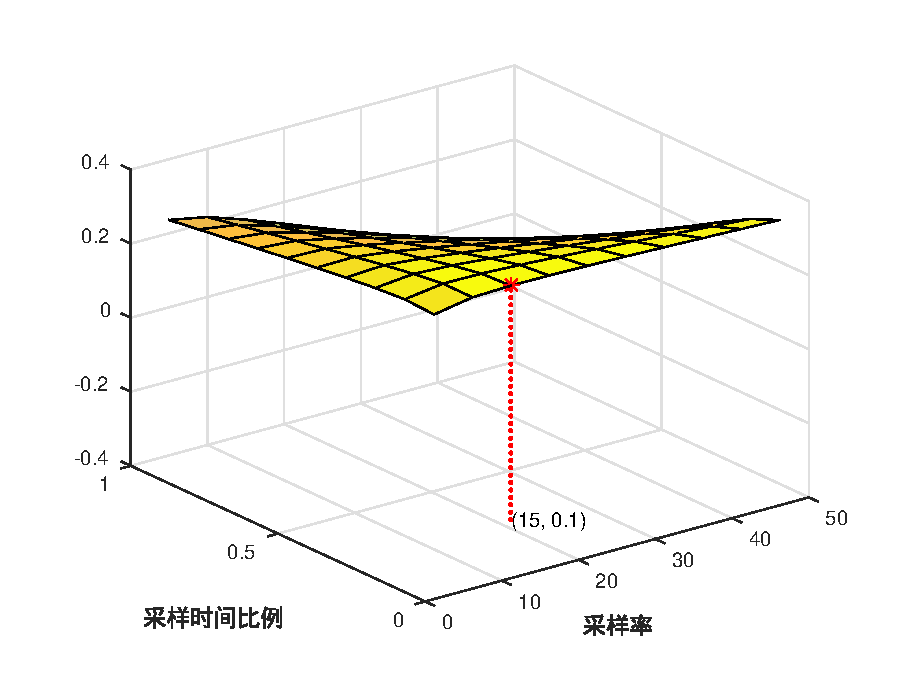
\includegraphics[width=0.3\textwidth]{object_static.eps}}
    \subfloat[行走状态的目标函数]{
    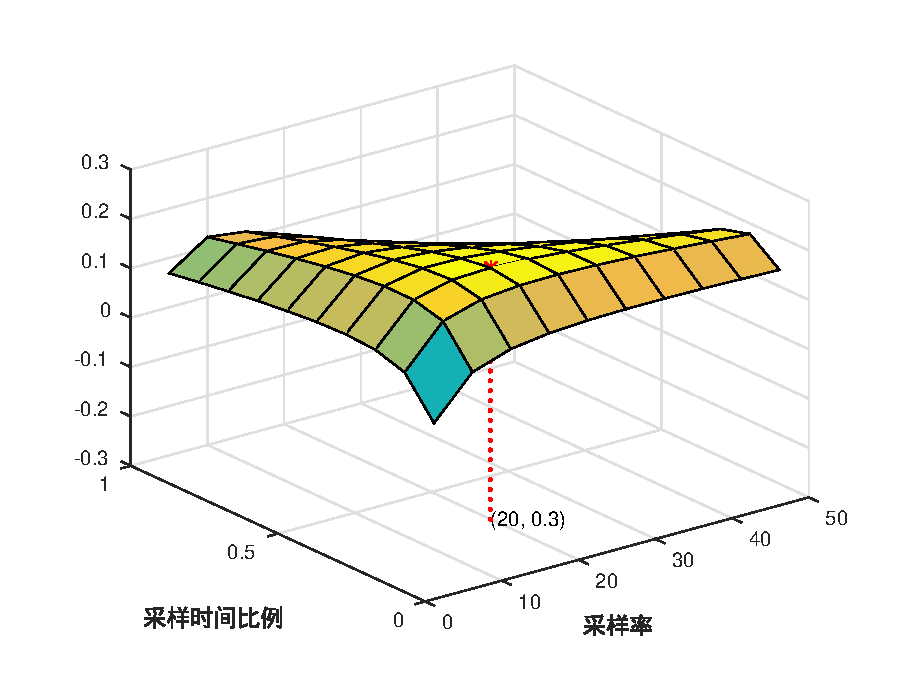
\includegraphics[width=0.3\textwidth]{object_walk.eps}}
    \subfloat[跑步状态的目标函数]{
    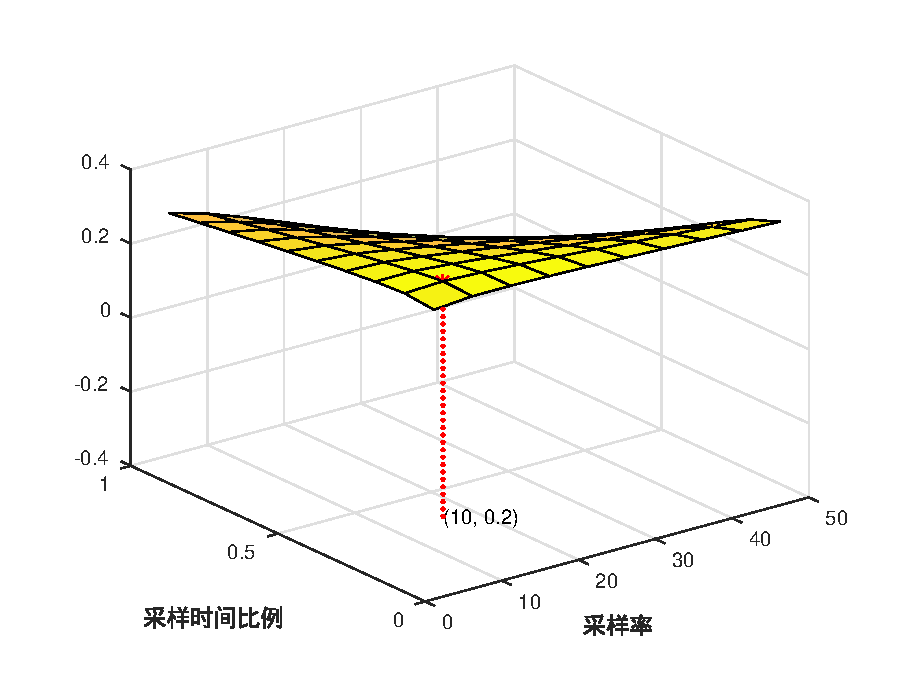
\includegraphics[width=0.3\textwidth]{object_run.eps}}
    \caption{仅使用时域特征时各行为状态的目标函数(1)}\label{object_function1}
\end{figure}

\begin{figure}[htb]
    \centering
    \subfloat[上楼状态的目标函数]{
    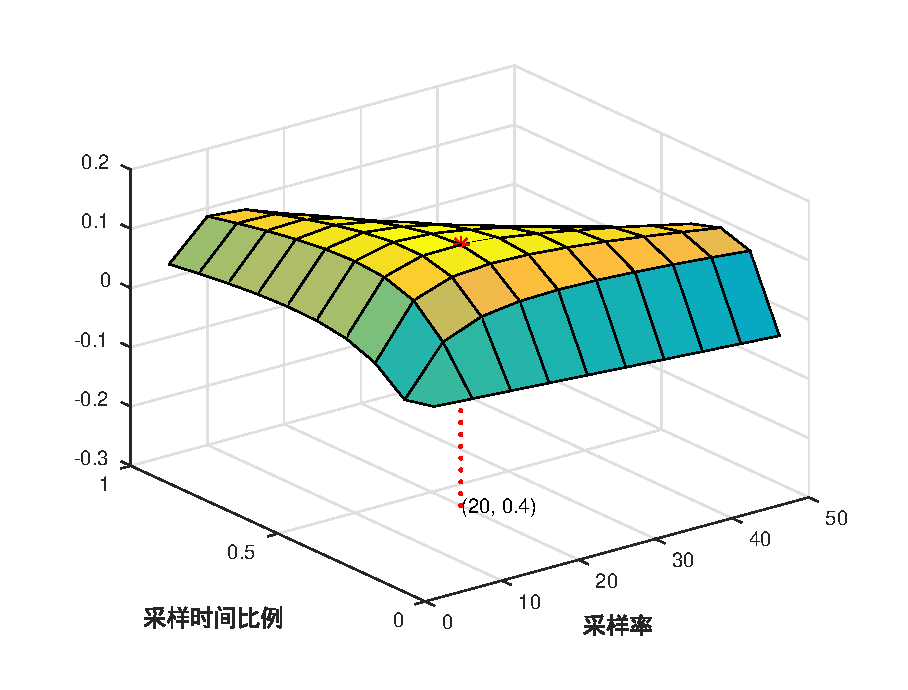
\includegraphics[width=0.3\textwidth]{object_ascend.eps}}
    \subfloat[下楼状态的目标函数]{
    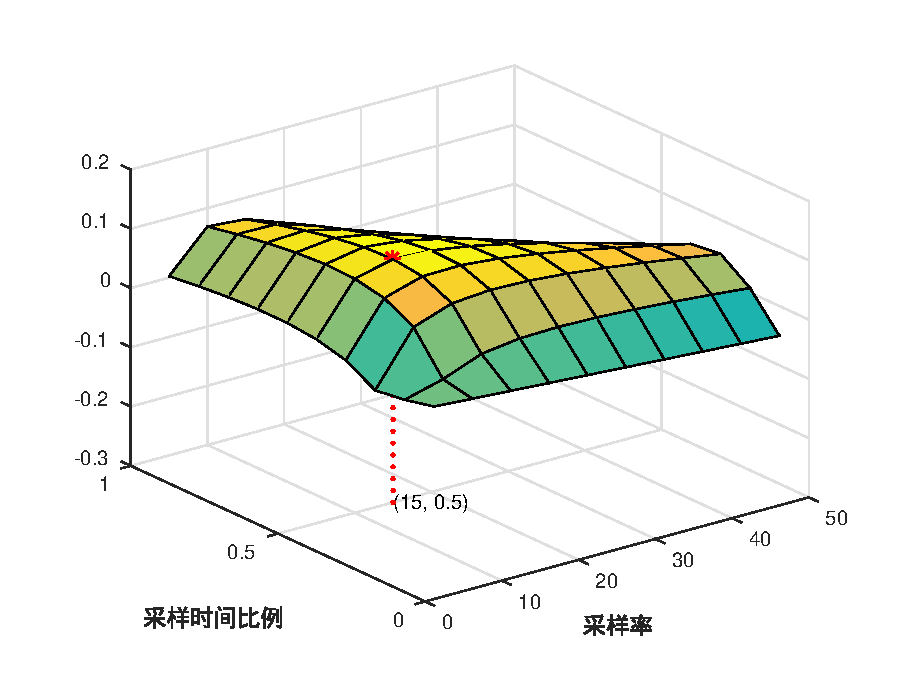
\includegraphics[width=0.3\textwidth]{object_descend.eps}}
    \caption{仅使用时域特征时各行为状态的目标函数(2)}\label{object_function2}
\end{figure}
\subsection{最优化问题求解}
\par 在通过实验测量求解获取能耗和准确率模型以后,就可以以当前电池电量等级为系数建立目标函数权衡二者关系,并通过求解关于目标函数的最优化问题就可以计算得到每类行为的识别策略。本文中,目标函数的权衡系数是随着电量变化而动态调整的,通过当前电量的百分比,向上取10的整数倍计算权衡系数,取值为0.1到1.0十个动态选择的范围。对于目标函数中的两个离散变量,即是否使用频域和自相关函数特征,本文通过将目标函数分为四种情况分别计算其最优解,然后再对四个最优值比较选择最优解,同时也确定了识别策略(\bm{$\widehat{f}$},\bm{$\widehat{\tau}$},\bm{$\widehat{\mu}$},\bm{$\widehat{\lambda}$}),其中采样率$\widehat{f_{ij}}$,采样时间比例$\widehat{\tau_{ij}}$,是否使用频域特征$\widehat{\mu_{ij}}$,是否使用自相关函数特征$\widehat{\lambda_{ij}}$,表示行为$i$在电量确定的权衡系数$\varphi (battery) = j/10$时的识别策略。

\par 首先本文以仅使用时域特征时,并且考虑在设定电量权衡系数$\varphi (battery) = 0.5$的情况为例,计算目标函数。五类行为状态下,目标函数取反以后与采样率的和采样时间比例的函数关系如图\ref{object_function1}(a)-(c)和图\ref{object_function2}(a)-(b)所示,其中在图中已经标出在仅使用时域特征时的各目标函数最优值以及其最佳采样率和采样时间比例。
%各行为状态下的目标函数图
\par 从图中可以看出,静止和跑步等区别较为明显的行为,对采样率和采样时间的依赖程度并不高,在较低的采样率和采样时间时具有较高的收益。而对于慢速动态行为,特别是上下楼时,当降低采样率和采样时间时到一定程度时,目标函数会急剧下降,说明此时的准确率降低的幅度较大,因此需要保证一定的采样率和采样时间。
\par 最后针对每一类行为求解目标函数的最优解,进而可以获得识别每一类行为的识别策略,识别策略如下表:
% 识别策略表格
\begin{table}[htb]
    \centering
    \caption{各电量状态下各行为的识别策略}
    \begin{tabular}{ccccccc}
    \toprule
    电量 & 静止 & 行走 & 跑步 & 上楼 & 下楼 \\
    \midrule
    10 & 10\%/5/T & 10\%/5/T & 10\%/5/T & 10\%/5/T & 10\%/5/T \\
    20 & 10\%/5/T & 10\%/10/TA & 10\%/5/T & 10\%/5/T & 10\%/5/T \\
    30 & 10\%/10/TA & 20\%/10/TA & 10\%/10/T & 30\%/10/TA & 30\%/5/TFA \\
    40 & 10\%/10/TA & 20\%/15/TA & 10\%/10/T & 30\%/10/TF & 40\%/5/TFA \\
    50 & 10\%/15/TA & 30\%/15/TA & 20\%/10/T & 40\%/10/TF & 50\%/5/TFA \\
    60 & 10\%/15/TA & 30\%/15/TA & 20\%/10/T & 50\%/10/TF & 60\%/5/TFA \\
    70 & 20\%/15/TA & 40\%/25/TA & 20\%/15/T & 60\%/10/TFA & 80\%/5/TFA \\
    80 & 20\%/15/TA & 50\%/25/TA & 30\%/15/T & 70\%/15/TF & 100\%/5/TFA \\
    90 & 20\%/25/TA & 60\%/25/TA & 30\%/15/TA & 100\%/15/TFA & 100\%/5/TFA \\
    100 & 30\%/25/TA & 70\%/50/TF & 40\%/15/TF & 1000\%/25/TFA & 100\%/5/TFA \\
    \bottomrule
    \end{tabular}
\end{table}

\par 其中每个策略的第一个变量是采样时间比例,第二个变量是采样率,单位是Hz,第三个是所使用的特征选择范围,T表示时域,F表示频域,A表示自相关函数有关的特征。从表格中可以看出,对于静止和跑步等区分较为明显的行为,采样时间不需要太长,所需要的特征也较为简单,而对于上楼和下楼区分不太明显的行为,则通常需要较长的采样时间,而且需要较多的特征,但是采样率要求不是太高。
\section{识别策略动态调整方案}
\par 在计算获取到每种情况下的识别策略以后,需要在人体行为识别过程中,根据上下文信息动态调整识别策略,以实现降低识别过程中能耗的目的。首先,应用需要检测手机电量的变化,当电量变化会引起权衡系数变化时也就说明识别策略也发生变化,此时需要作出线上实时调整。其次,应用需要根据当前的行为识别结果决定下一时刻的识别策略,其中最关键的问题在于判定行为的转变,即判定行为状态是否确定转变,需要对策略作出调整。为此,本文提出一种识别策略的动态调整方案,其流程框图如图\ref{dapte_strategy}所示。
%识别策略动态调整方法框图
\begin{figure}[htp]
\centering
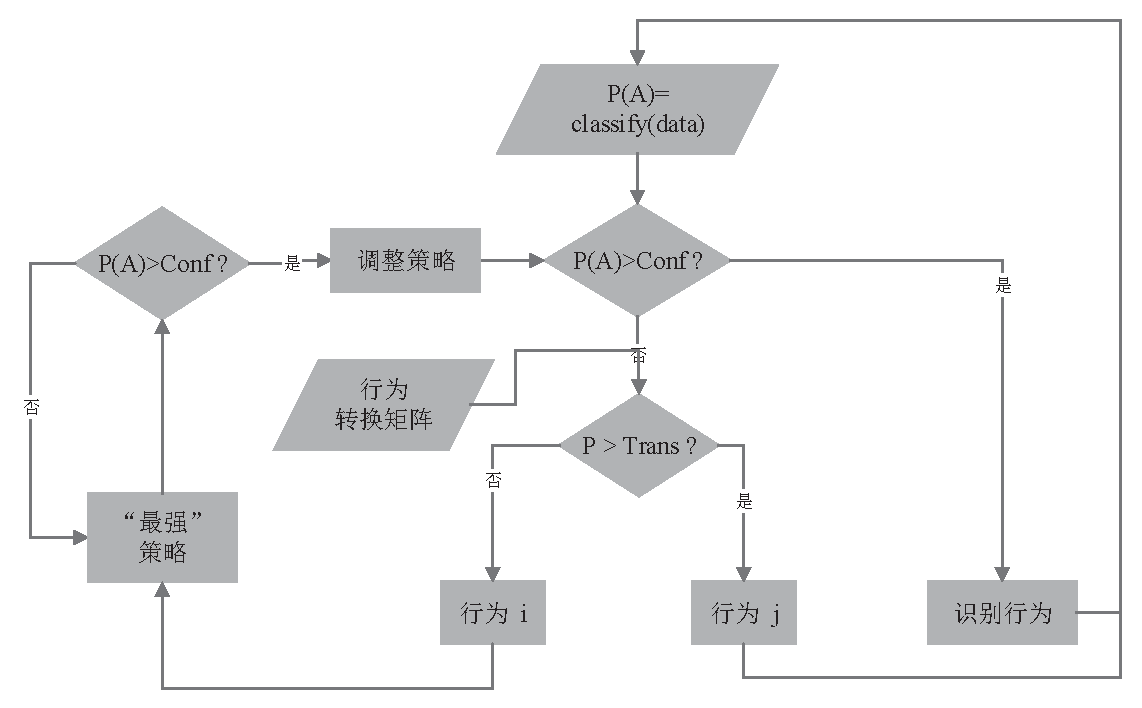
\includegraphics[width = 0.8\textwidth]{dapte_strategy.eps}
\caption{识别策略的动态调整方案框图}\label{dapte_strategy}
\end{figure}

\par 在我们的识别框架中,分类方法继续使用前面介绍的随机森林的算法。随机森林分类方法通常会使用100棵决策树,每棵决策树从特征集中随机选择一定数量的特征组成特征向量进行决策分类,最后获得100个分类结果,随机森林算法将会选择其中比例最大的类别作为最终的分类结果。而在本文的方案框架将随机森林中所有决策树的识别结果中某类行为$i$所占的比例定义为$P(A_i)$, 表示分类器对该实例识别为行为$i$的概率, $Conf_{low}$为设定阈值,表示认为可以确定该行为的最低置信概率。若某一次识别过程中最终的识别行为的概率超过阈值$Conf_{low}$则确定为该识别结果,下一窗口时间使用该行为的识别策略。若小于$Conf_{low}$,则计算行为转换概率$P_{ij}$,即当前行为$i$转换为行为$j$的概率,其计算公式可以表示为:
\begin{equation}
	max \{P_{ij} = P(A_j)a_{ij}\}, \quad j = 1 \cdots, i-1, i+1, \cdots, N
\end{equation}
其中, $i$表示前一次识别的行为,$a_{ij}$为行为转换矩阵中行为$i$转换为行为$j$的概率。若$P_{ij}$大于设定阈值$Trans_{low}$ ,则判定发生行为转变,下一窗口时间调整为行为$j$的识别策略,否则,$P_{ij}$小于$Trans_{low}$则表示无法判定已经发生了明确的行为转换,此次判定为上一窗口的行为,即行为$i$,下一窗口时间使用“最强”识别策略,即最大采样率和采样时间以及最大的特征选择范围,持续使用该策略识别分类,直到识别的概率超过置信概率阈值 ,则调整为对应行为的识别策略,继续下一窗口的识别。

\section{对比实验结果}
\par 为了验证本文的识别策略动态调整方案的有效性,我们通过实际生活中的监测实验,与没有使用识别策略调整时的情况对比,分析识别策略调整方案在能耗与准确率方面的性能。同时,本文也同之前的降低能耗的研究文献作出对比。在文献\cite{modelVarialb}中,作者研究了离散的识别策略调整方案,该文献中作者考虑了采样率和特征集的选择等变量,他们采用选择若干离散的采样率以及有限个数的特征集选择范围,然后将二者组成有限数量的二元组,最后通过权衡识别准确率和能耗,从中选择最佳的二元组最为最佳的识别策略。本小节剩余部分将通过对比实验作出本文方法与文献中方法的性能比较。

\subsection{实验设定}
\par 首先,该部分对比实验依然使用Google公司设计的Nexus5智能手机运行行为识别手机应用。实验对比对象为未实现策略动态调整的方案,离散的策略调整方案以及本文的动态调整方案,因此实验过程中有三部手机分别同时运行行为识别应用,其中第一部手机应用没有使用动态调整方案,后两部手机应用分别实现了文献\cite{modelVarialb}中和本文中的策略调整方案。实验的对比指标为应用的识别准确率和能耗两项。
\par 实验参与者同时佩戴三部手机分别运行上述三款应用,在没有干扰的情况下随机执行静止、行走、跑步、上楼和下楼五种类型的行为。为有效计算识别准确率,在实验过程中实时记录实验参与者的实际行为。实验的限定时间分别设置为10, 20, 30, 40, 50分钟,分别计算在限定时间内的准确率和能耗。本文实验共有6人参与,并计算准确率和能耗的平均值作为最终结果用于对比分析。
\subsection{实验结果与分析}
\par 行为识别手机应用在分别采用本文的识别策略调整方案,离散的识别策略调整方案\scite{modelVarialb}以及没有采用策略调整方案的情况下,同时对6人进行行为识别,相应的准确率和能耗的平均值分别表格\ref{final_precision}和\ref{final_energy},三类情况下的识别准确率和识别能耗如图\ref{com_result}所示。

\begin{table}[htb]
    \centering
    \caption{对比实验中三种情况下的识别准确率}\label{final_precision}
    \begin{tabular}{ccccccc}
    \toprule
    时间 & 10 & 20 & 30 & 40 & 50 \\
    \midrule
    没有策略调整 & 0.9524 & 0.9637 & 0.9611 & 0.9680 & 0.9622 \\
    本文的策略调整 & 0.9294 & 0.9315 & 0.9394 & 0.9441 & 0.9440 \\
    离散的策略调整 & 0.9252 & 0.9288 & 0.9335 & 0.9306 & 0.9373 \\
    \bottomrule
    \end{tabular}
\end{table}

\begin{table}[htb]
    \centering
    \caption{对比实验中三种情况下的识别能耗}\label{final_energy}
    \begin{tabular}{ccccccc}
    \toprule
    时间 & 10 & 20 & 30 & 40 & 50 \\
    \midrule
    没有策略调整 & 9.78 & 18.3 & 25.8 & 36.1 & 45.2 \\
    本文的策略调整 & 6.16 & 13.2 & 18.8 & 26.3 & 34.7 \\
    离散的策略调整 & 7.6567 & 15.6 & 19.9 & 27.9 & 38.6 \\
    \bottomrule
    \end{tabular}
\end{table}

\begin{figure}[htb]
    \centering
    \subfloat[对比实验中三种情况下的识别准确率]{
    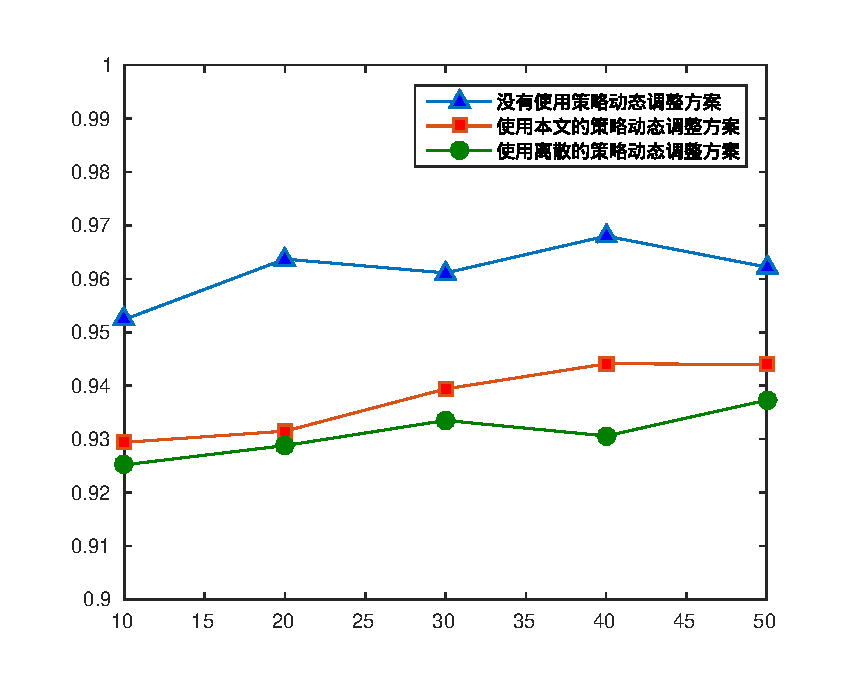
\includegraphics[width=0.45\textwidth]{precision.eps}}
    \subfloat[对比实验中三种情况下的识别能耗]{
    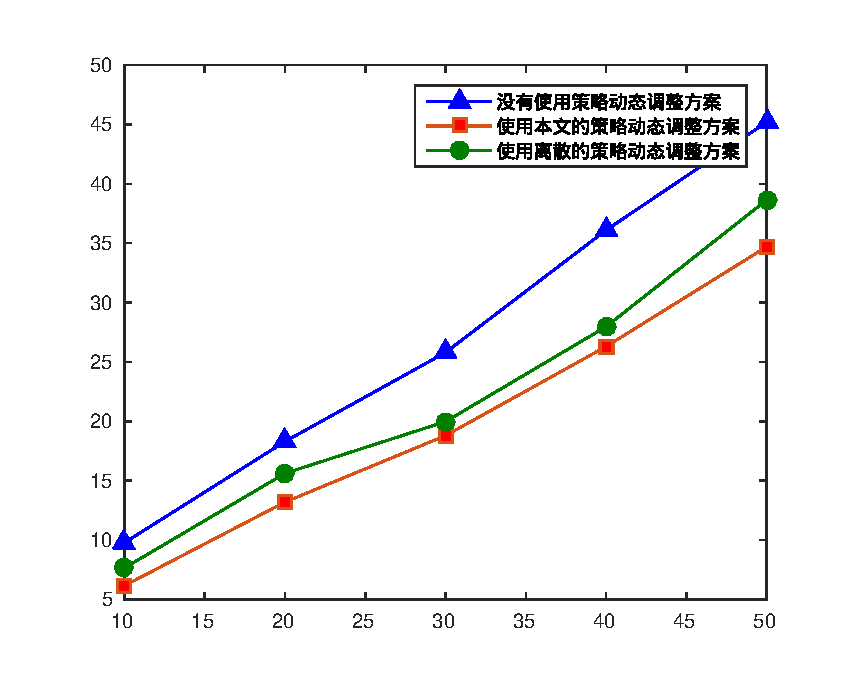
\includegraphics[width=0.45\textwidth]{energy.eps}}
    \caption{对比实验三种情况下的对比结果}\label{com_result}
\end{figure}

\par 如图\ref{com_result}所示,在使用策略动态调整的情况下,识别准确率有所下降,但是幅度不大,并且保持在90\%以上,而从图(b)可以看出在使用识别策略调整的情况下,能耗有明显降低,相比与没有使用调整策略的情况,使用本文的策略调整方案能耗平均降低了28.48\%,而相比于之前的离散的策略调整方案,识别能耗也降低了11.43\%,从而说明了本文所提出识别策略调整方案的有效性。

\section{本章小结}
\par 本章主要介绍了我们对降低行为识别过程中智能手机能耗的研究。降低能耗的基本思想是通过调节采样率等变量权衡行为识别过程中能耗与准确率之间的关系,进而选择一种识别策略执行行为识别。本章首先对能耗和准确率建立了数学模型,研究二者与采样率、采样时间以及特征选择范围之间的函数关系,并以电量为权衡系数结合二者建立目标函数,从而将识别策略选择转化为求解关于目标函数的最优化问题。然后通过实验测量的方法求解数学模型中的参数,为每一种行为求解出一种最佳的识别策略。同时,为了在识别过程中合理调整策略,本文介绍了一种结合行为转换概率和识别结果的转换判定方法,动态地调整识别策略进行行为识别。最后,本章还通过设置对比实验分析了本文所提出的识别策略动态调整方法的有效性。
  \chapter{人体行为识别系统设计介绍}
\par 针对基于智能手机的行为识别的研究,本文所提出了的两层多策略的行为识别方案框架以及降低识别能耗的最佳策略动态调整方法,为验证它们的有效性和实用性,本文实现了一款可以运行于Android手机操作系统上的行为识别应用。之所以选择Android手机操作系统,一方面是因为它是开源且成熟的智能手机操作系统,提供了丰富的应用编程接口,基于该操作系统的应用较多,基于Android系统开发行为识别应用容易开发实现。另一方面是因为Android操作系统的市场占有量最高,是目前应用最为广泛的手机操作系统,因此基于Android系统开发行为识别应用,也更具有代表性。
\par 本文所实现的行为识别应用可以使用智能手机内置传感器获取关于人体行为的相关传感器数据,并通过已经实现的分类算法对用户当前行为作出识别判断。与此同时,该应用还具有与远端服务器通信的功能,可以保存用户运动数据以及查询用户的历史运动数据等,从而构成一套较为完整的人体行为识别系统。行为识别应用的框架结构如图所示。
%应用框架结构
\begin{figure}[ht]
\centering
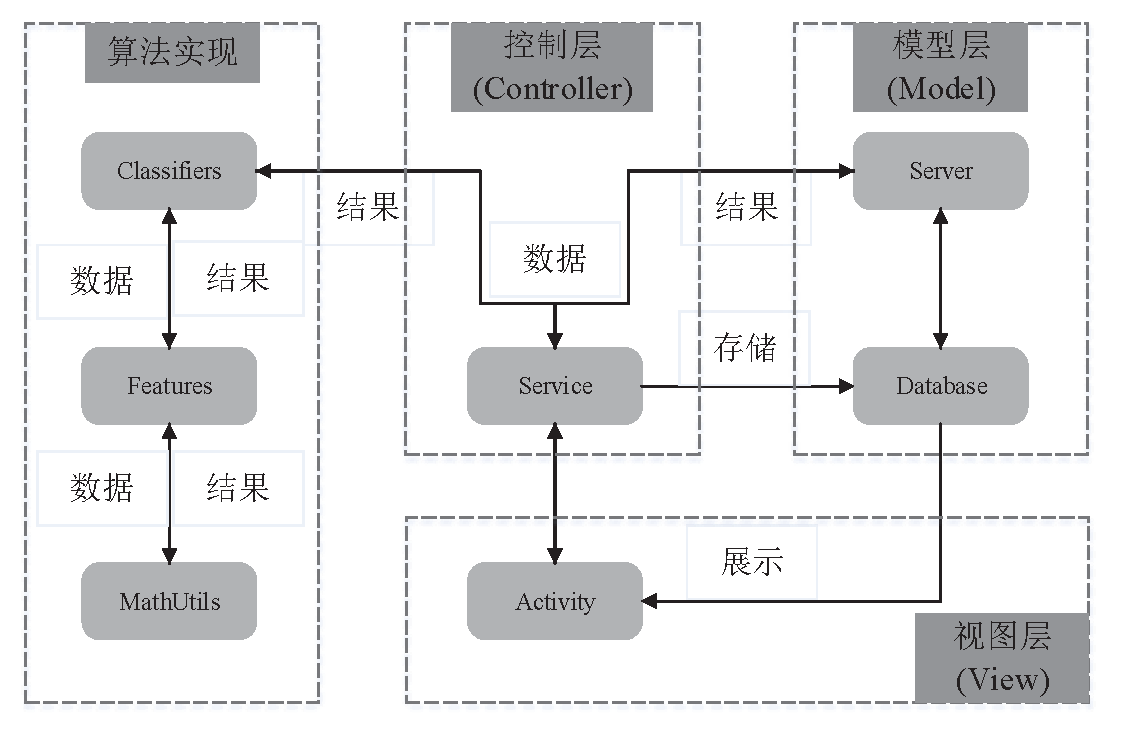
\includegraphics[width = 0.8\textwidth]{app_framework.eps}
\caption{最佳策略的动态调整方案框图}
\end{figure}
\par 行为识别应用共分为控制层,分类算法,模型层和视图层四部分。其中,由于本文的研究重点是基于智能手机的行为识别算法以及降低能耗的最佳策略调整方法,因此本文将应用框架的分类算法实现部分从模型层中分离出来单独介绍。控制层主要负责传感器的数据获取以及协调其他各部分的功能并与之通信,模型层主要负责数据的加载与保存,以及本地数据与远端服务器数据的同步等,视图层则只负责与用户的交互以及识别结果的展示。本章将从这四部分介绍人体行为识别系统的具体功能。
\section{控制层部分}
\par 行为识别应用的控制层主要由一个Android系统中的Service组成,主要负责数据获取以及统一协调其他功能模块两方面的功能。Service是Android操作系统中的重要组件之一,它没有可视化界面,是一种运行于后台的服务程序,主要负责不需要用户交互的长期运行任务。本文中的应用程序使用Service主要负责获取数据并协调控制其他功能模块。

\begin{itemize}
	\item 选择最佳策略
\end{itemize}
\par 该部分实现本文提出的最佳策略动态调整方法,根据第四章中介绍的方法根据识别结果和行为转换矩阵计算下一窗口时间内最佳的识别策略,包括数据采样率,采样时间比例以及是否使用频域和自相关函数特征。策略的前两部分传递至数据获取功能模块,控制数据采集,后面两部分传递至算法实现部分,控制特征选择范围。
\begin{itemize}
	\item 获取传感器数据
\end{itemize}
\par 数据获取功能模块主要负责采集以指定采样率和采样时间获取指定传感器的数据。一方面,在Service内部通过定义两个定时器控制采样时间,一个定时器负责控制数据窗口的大小也是行为识别判定一次的时间窗口大小,另一个定时器负责采样时间的比例,即控制传感器进入休眠状态,等待下一个窗口时间开始时唤醒。另一方面,在Service内部通过获取Android系统提供的SensorManager服务,统一管理传感器的操作,本文主要使用SensorManager获取指定传感器对象,同时根据两个定时器切换这些传感器工作和休眠的状态以及算法所设定的采样率。
\begin{itemize}
	\item 协调控制其他功能模块
\end{itemize}
\par 除数据获取以外,控制层的Service的关键作用在于作为整个应用的枢纽,负责协调控制其他各个功能模块,包括将从传感器采集得到运动数据传递至算法实现部分对用户当前行为作出判断,并将识别结果送至视图层部分展示给用户,同时还负责将结果保存至本地数据库以及远端服务器等。其具体控制功能包括以下部分:
\begin{itemize}
	\item 控制算法实现部分:由定时器控制时间窗口大小,周期性地向算法实现部分传递传感器数据,并获取该窗口时间内的识别结果;
	\item 控制模型层部分:周期性地将识别结果保存至本地数据库,并在适当机会同步本地数据库与远端服务器的数据。
	\item 控制视图层部分:一方面负责接收视图层传递进来的用户交互事件命令,另一方面周期性地向视图层传递识别结果。
\end{itemize}
\section{分类算法实现部分}
\par 本部分主要实现第三章介绍的两层多策略的行为识别方案。该部分主要包括分类算法模块Classifier,特征提取与选择模块Features和数学工具模块MathUtils三部分,各部分的具体功能如下:
\begin{itemize}
	\item 分类算法模块:该部分负责接收Service传递进来的传感器数据并提供识别结果,内部包括实现的两层框架以及随机森林分类器,通过使用体征提取与选择模块提供的特征向量对当前时间窗口行为分类,计算最后识别结果;
	\item 特征提取与选择模块:该部分负责接收分类算法模块传递的传感器数据以及指定的特征序号计算指定特征,组成特征向量,返回至分类算法模块,用于行为分类;
	\item 数学工具:该部分负责提供各类数学计算工具,主要包括计算最值,均值,快速傅里叶变换,自相关函数等静态方法,为特征提取以及分类提供数学工具支持。
\end{itemize}
\section{模型层部分}
\par 由于本文将分类的业务逻辑已经单独提出在分类算法部分介绍,模型层部分则只需要负责对数据的存储和加载功能即可。对于数据的存储,本文使用Android系统内集成的SQLite数据库建立本地数据库存储行为数据。SQLite是一款轻型数据库,占用资源相对较少,常用于嵌入式设备。Android操作系统已经集成了SQLite数据库,使用该数据库可以方便地在手机端存储大量数据。Android操作系统提供有SQLiteOpenHelper工具类负责建立和更新数据库,同时也提供了一些编程接口,可以方便地使用SQL语句执行建表以及查询,插入,删除和更新数据等操作。
\par 本文所实现的应用需要存储的数据十分简单,只需要存储用户的行为信息即可。因此本应用所建立的数据库中包含用户表和行为表两个数据表。
\begin{itemize}
	\item 用户数据表$users$, 包括用户序号$user\_id$,用户名$user\_name$和密码$password$三个字段,用于记录用户信息以及登录过程的验证。
	\item 行为数据表$activities$,包括序号$\_id$, 用户序号$user\_id$,行为$activity$,时间$time$和是否已与服务器同步$is\_sync$五个字段,用于记录实时识别的行为信息。
\end{itemize}
\par 该应用的模型层部分对外提供操作数据库时的增删改查接口,便于其他部分对数据的操作。在识别过程中,由Service控制插入实时识别的行为数据,并且用户还可以通过视图层部分提供的用户界面操作控制数据的查询,删除和更新等。除此以外,Service还会在网络允许状态下负责本地数据库与远端服务器数据的同步。
\section{视图层部分}
\par 行为识别应用的界面层部分主要提供向用户展示识别结果以及为用户提供交互操作接口的功能。图\ref{screenshot1}(a)和(b)分别为手机应用的登录界面和初始化界面。用户登录以后进入初始化界面,此时应用会执行加载分类模型等一系列初始化操作,在初始化界面,开始按钮可以控制识别过程的开始与停止,查询按钮可以用于控制查询历史行为记录。
\begin{figure}[htb]
    \centering
    \subfloat[登录界面]{
    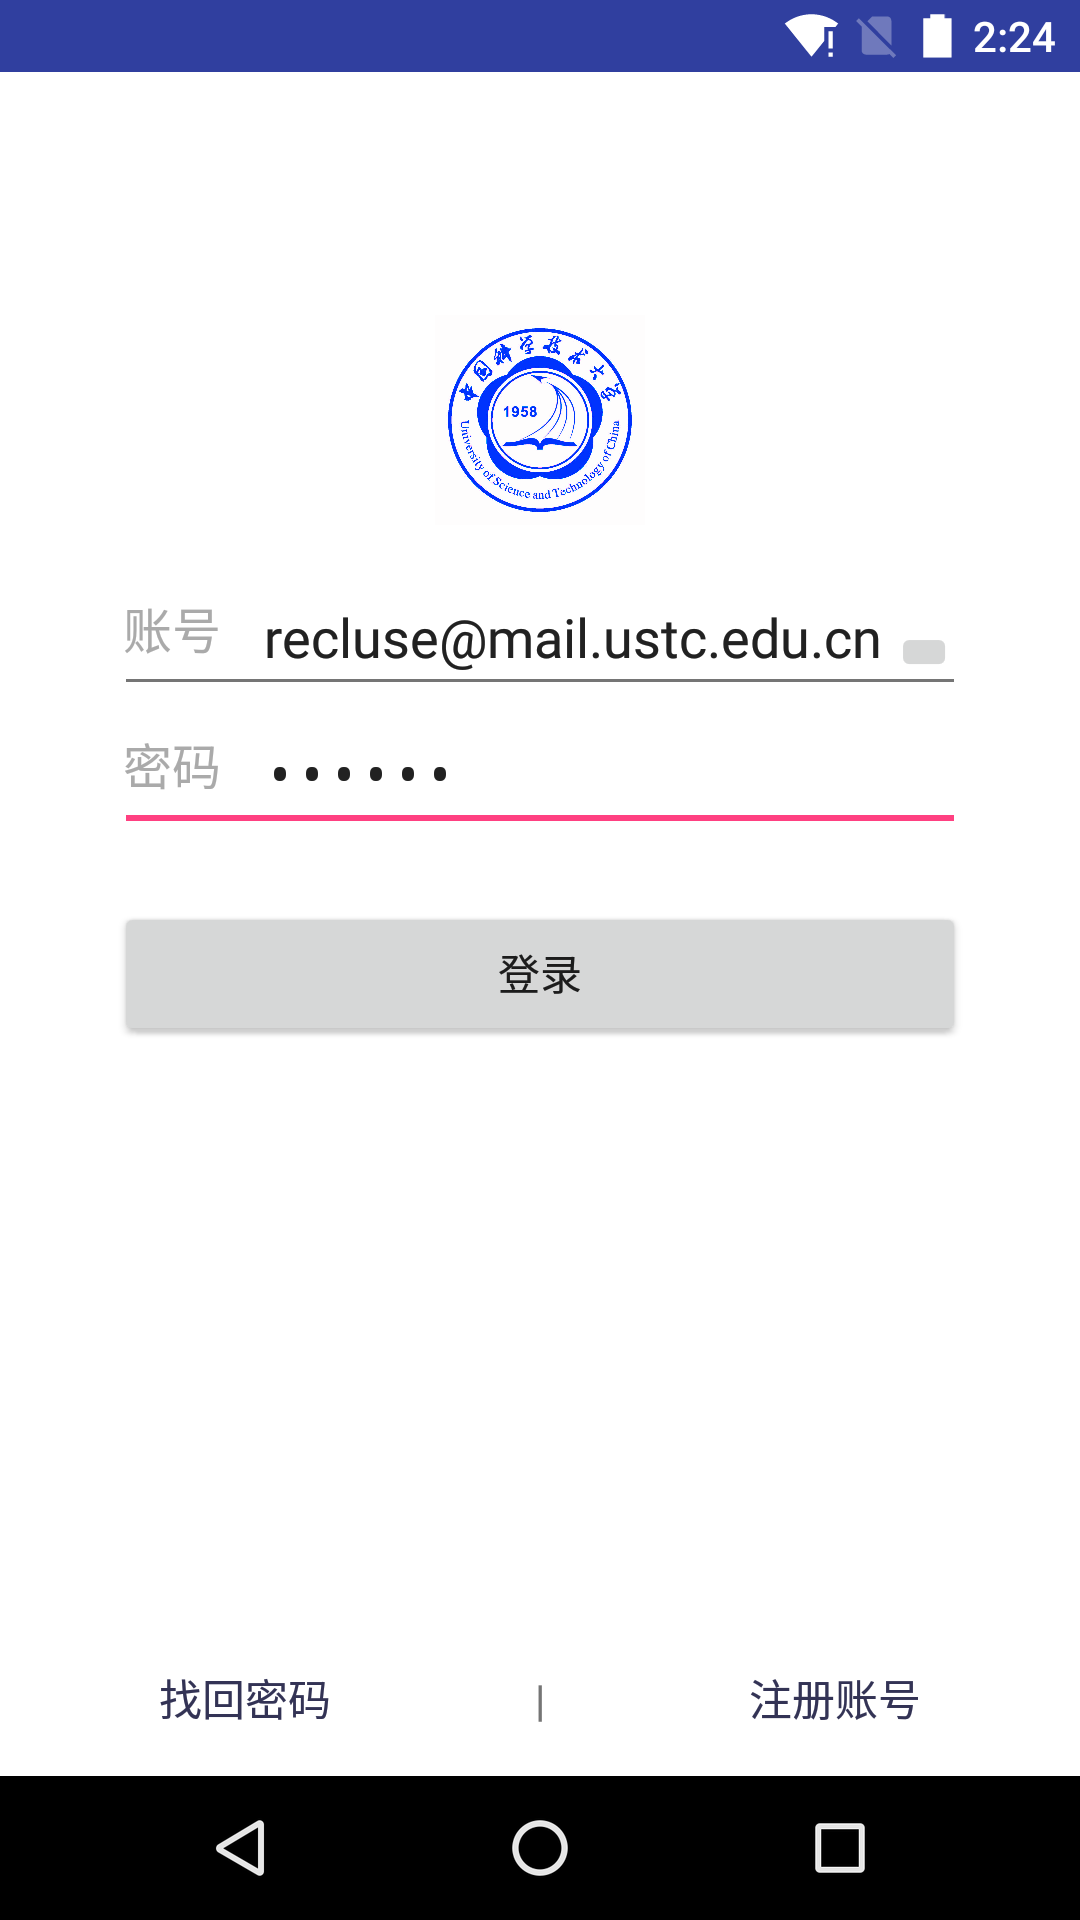
\includegraphics[width=0.3\textwidth]{login.png}}
    \subfloat[初始化界面]{
    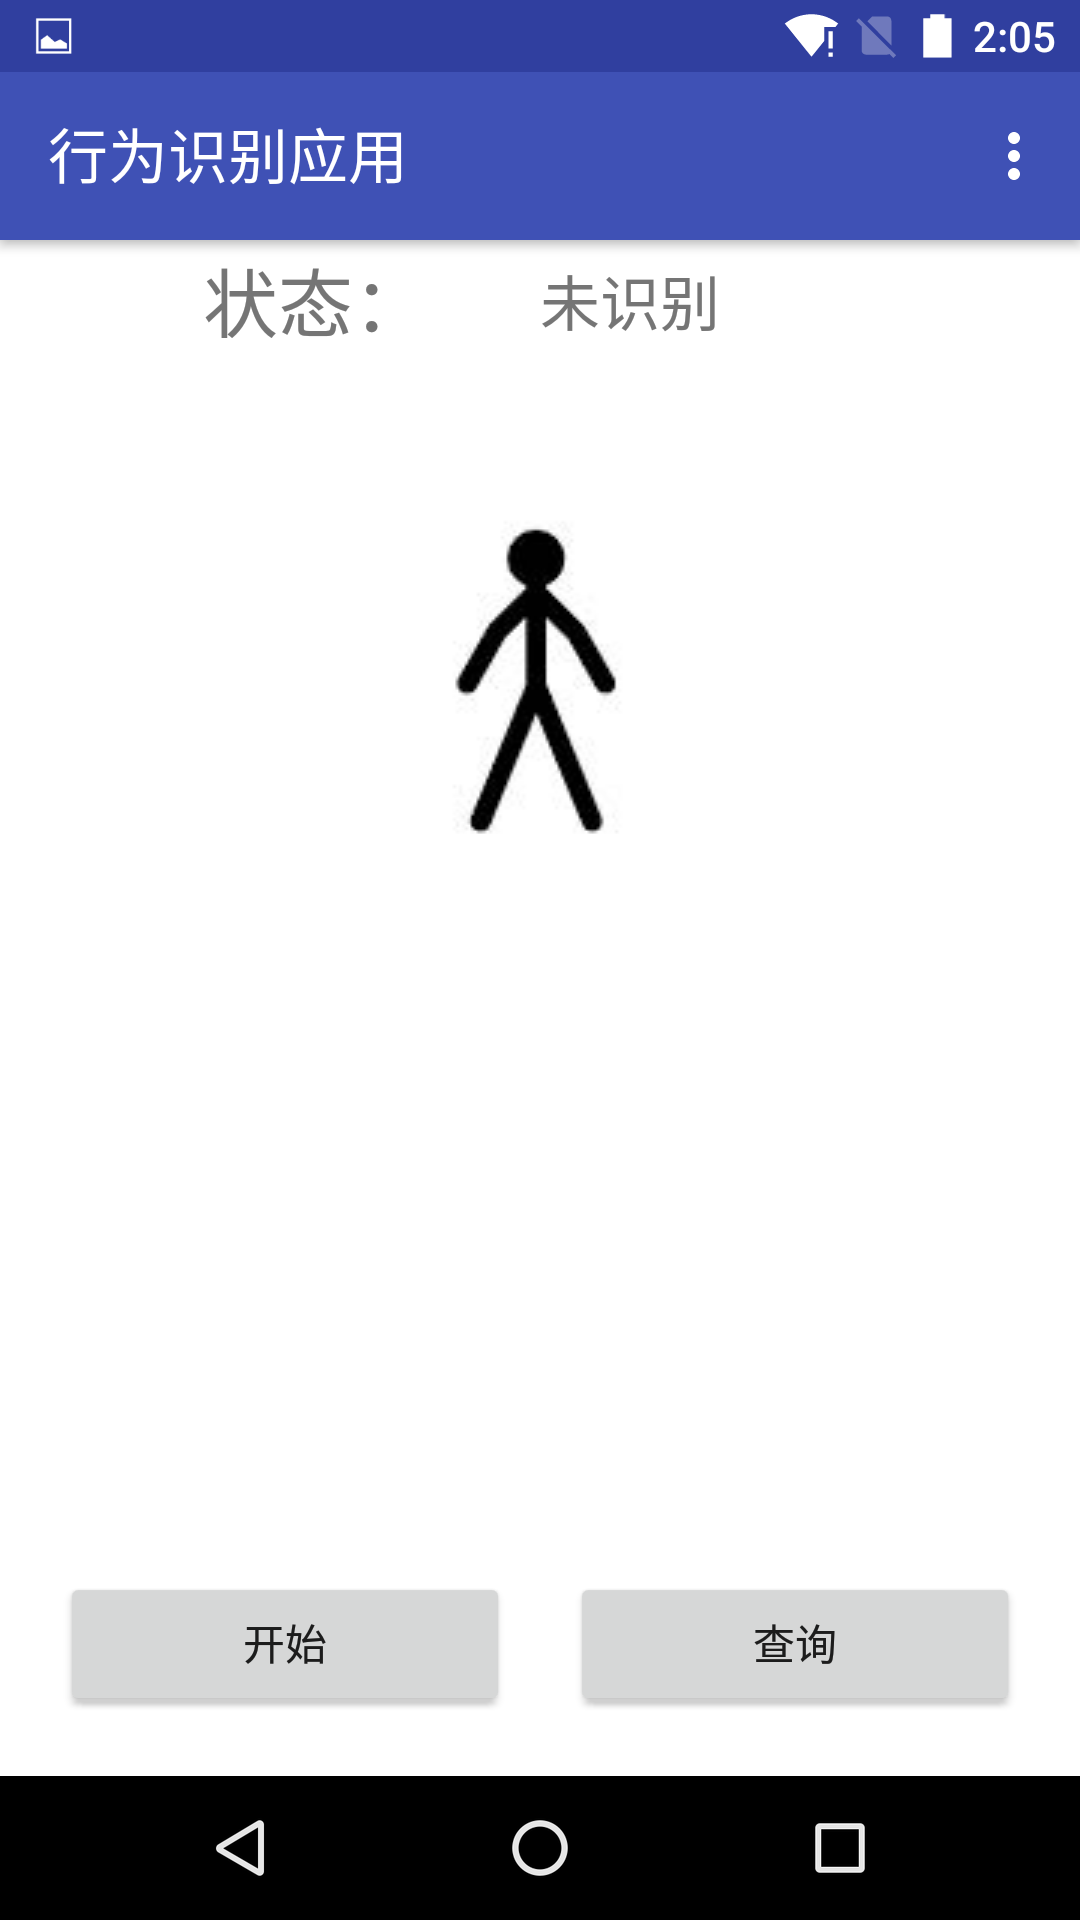
\includegraphics[width=0.3\textwidth]{init.png}}
    \caption{行为识别应用的部分界面}\label{screenshot1}
\end{figure}
\par 该行为识别应用提供两个展示识别结果的界面,一是如图\ref{screenshot2}(a)所示的行为GIF动画展示,二是如图\ref{screenshot2}(b)所示的以表格形式展示历史行为记录并随着识别过程实时更新曲线,通过查询/返回按钮可以控制两个界面的切换。同时该应用提供了历史记录的查询功能,通过菜单选项中提供的设置开始和结束时间,查询过去某一段时间的行为记录,记录以表格形式展示,在清除查询后表格恢复显示当前的实时行为记录。
\begin{figure}[htb]
    \centering
    \subfloat[行为GIF动画展示]{
    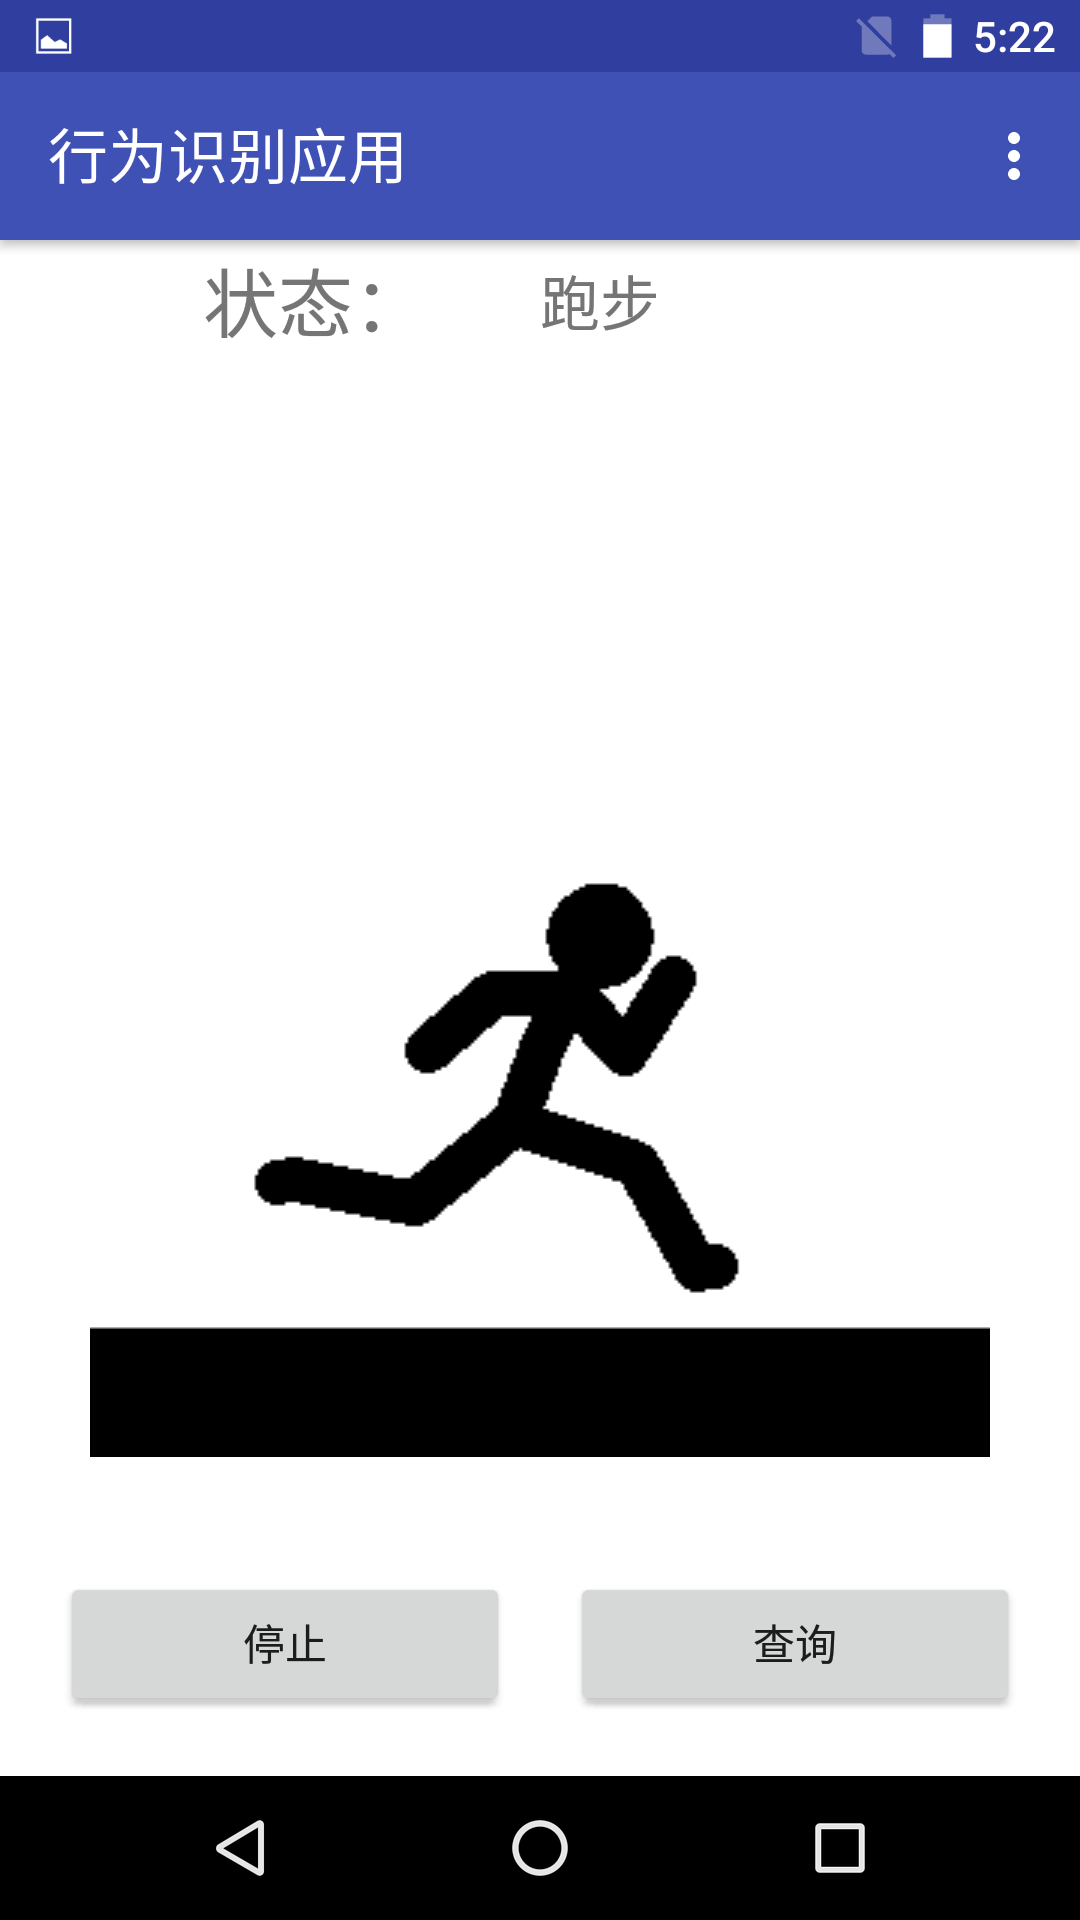
\includegraphics[width=0.23\textwidth]{run.png}}
    \subfloat[历史行为记录展示]{
    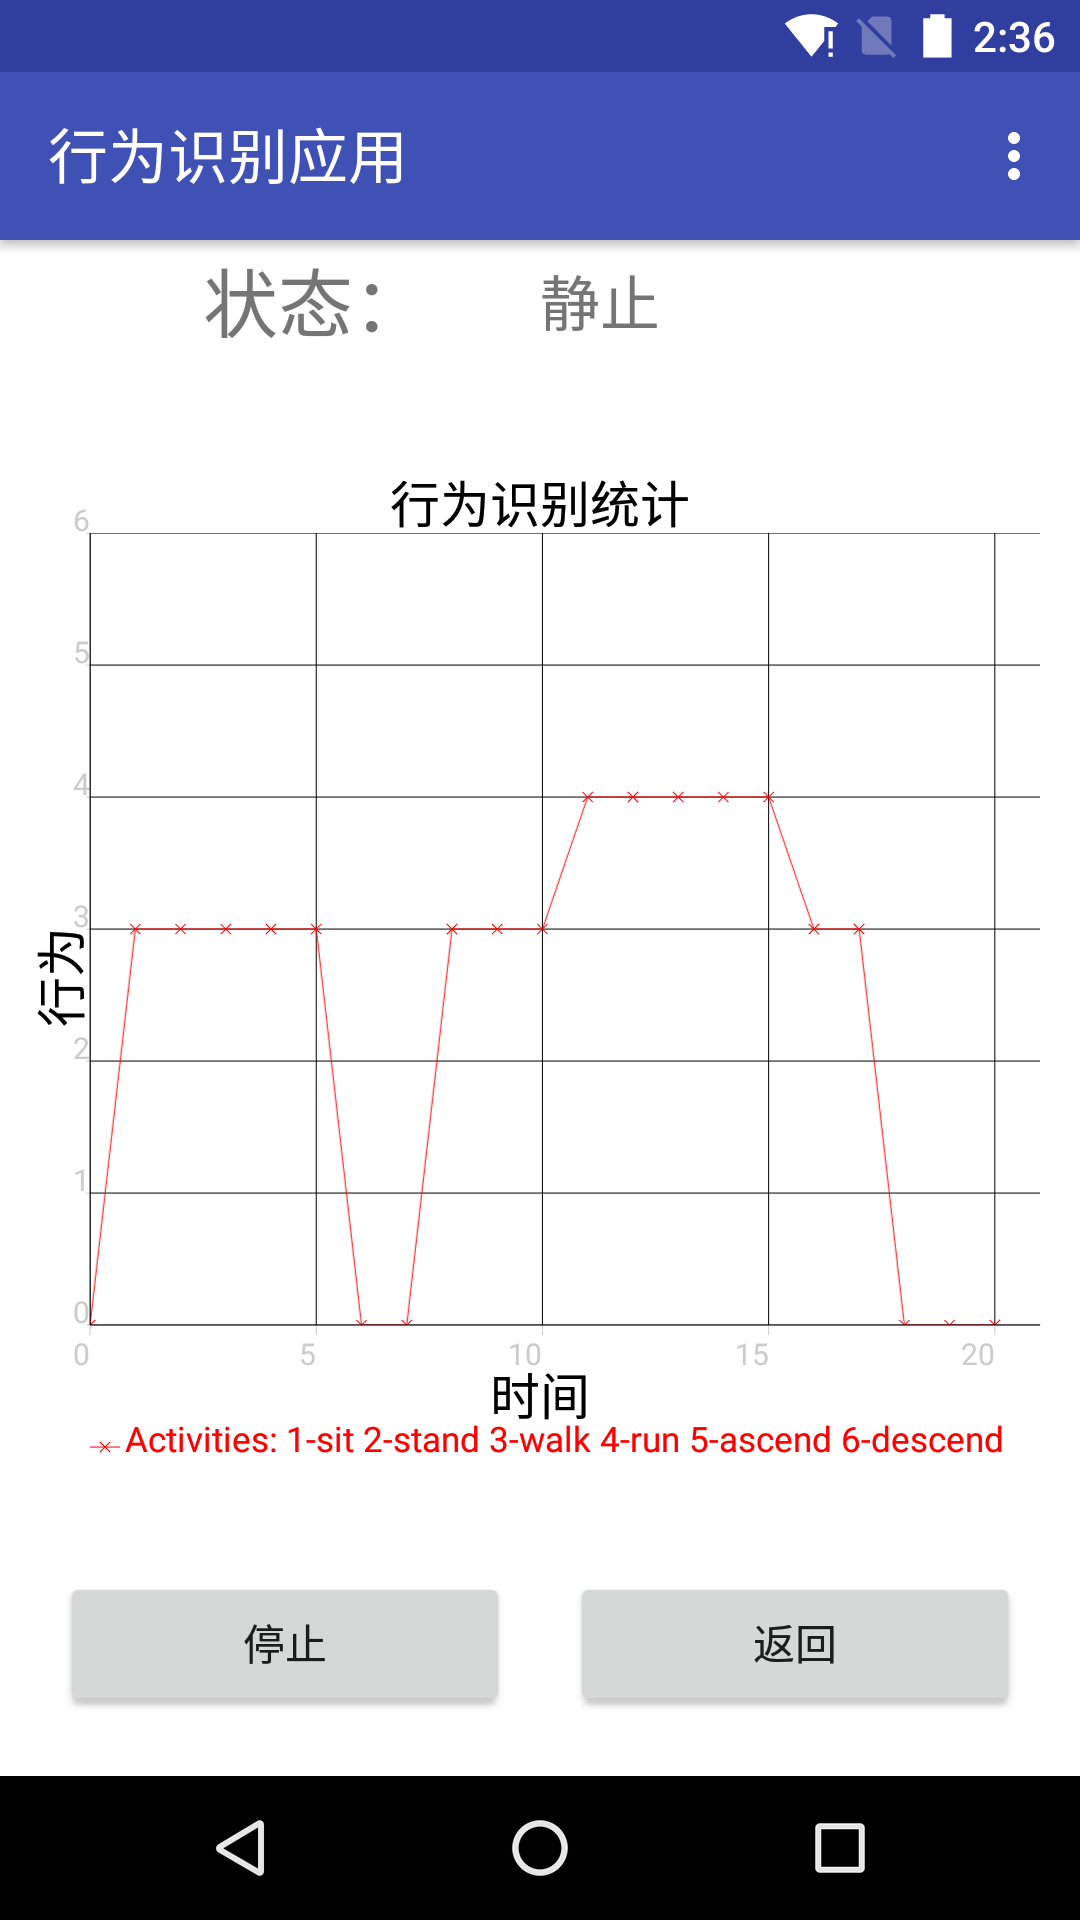
\includegraphics[width=0.23\textwidth]{query.png}}
    \subfloat[菜单选项]{
    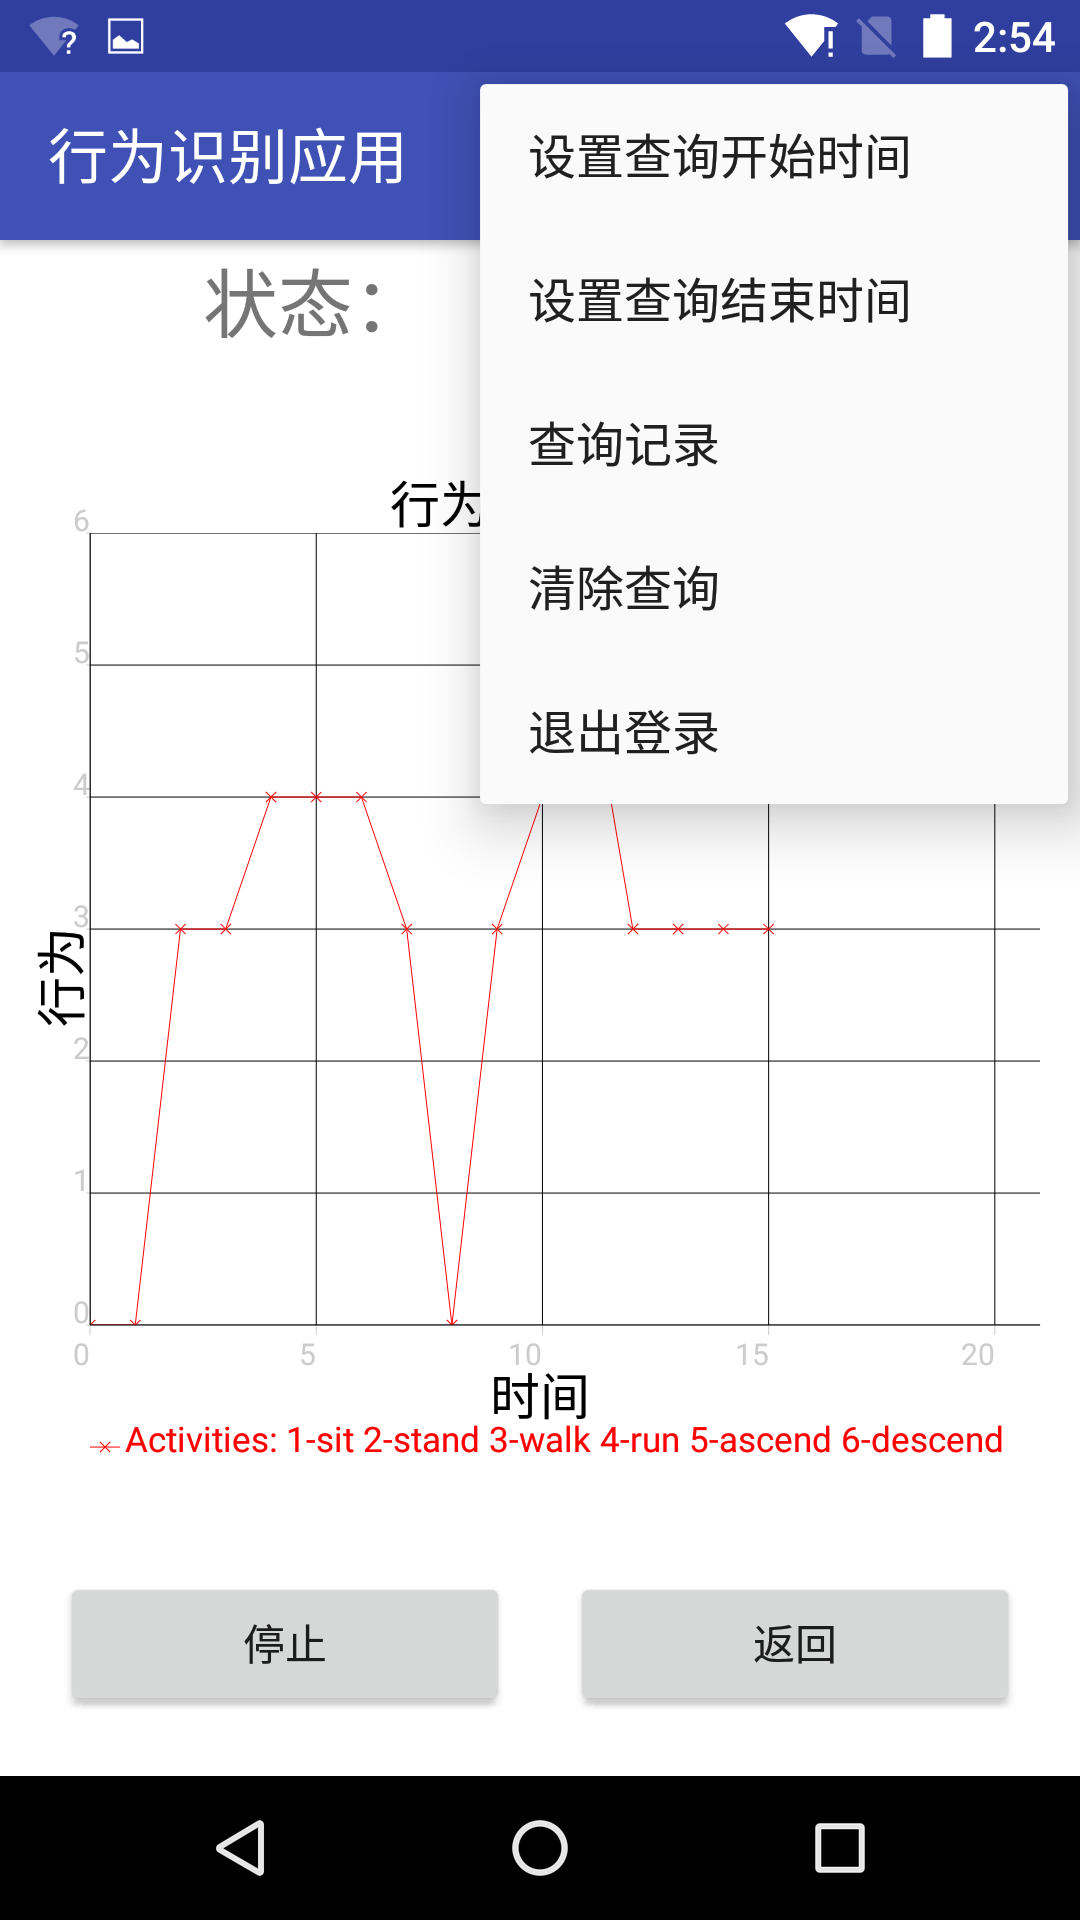
\includegraphics[width=0.23\textwidth]{menu.png}}
    \subfloat[时间设置对话框]{
    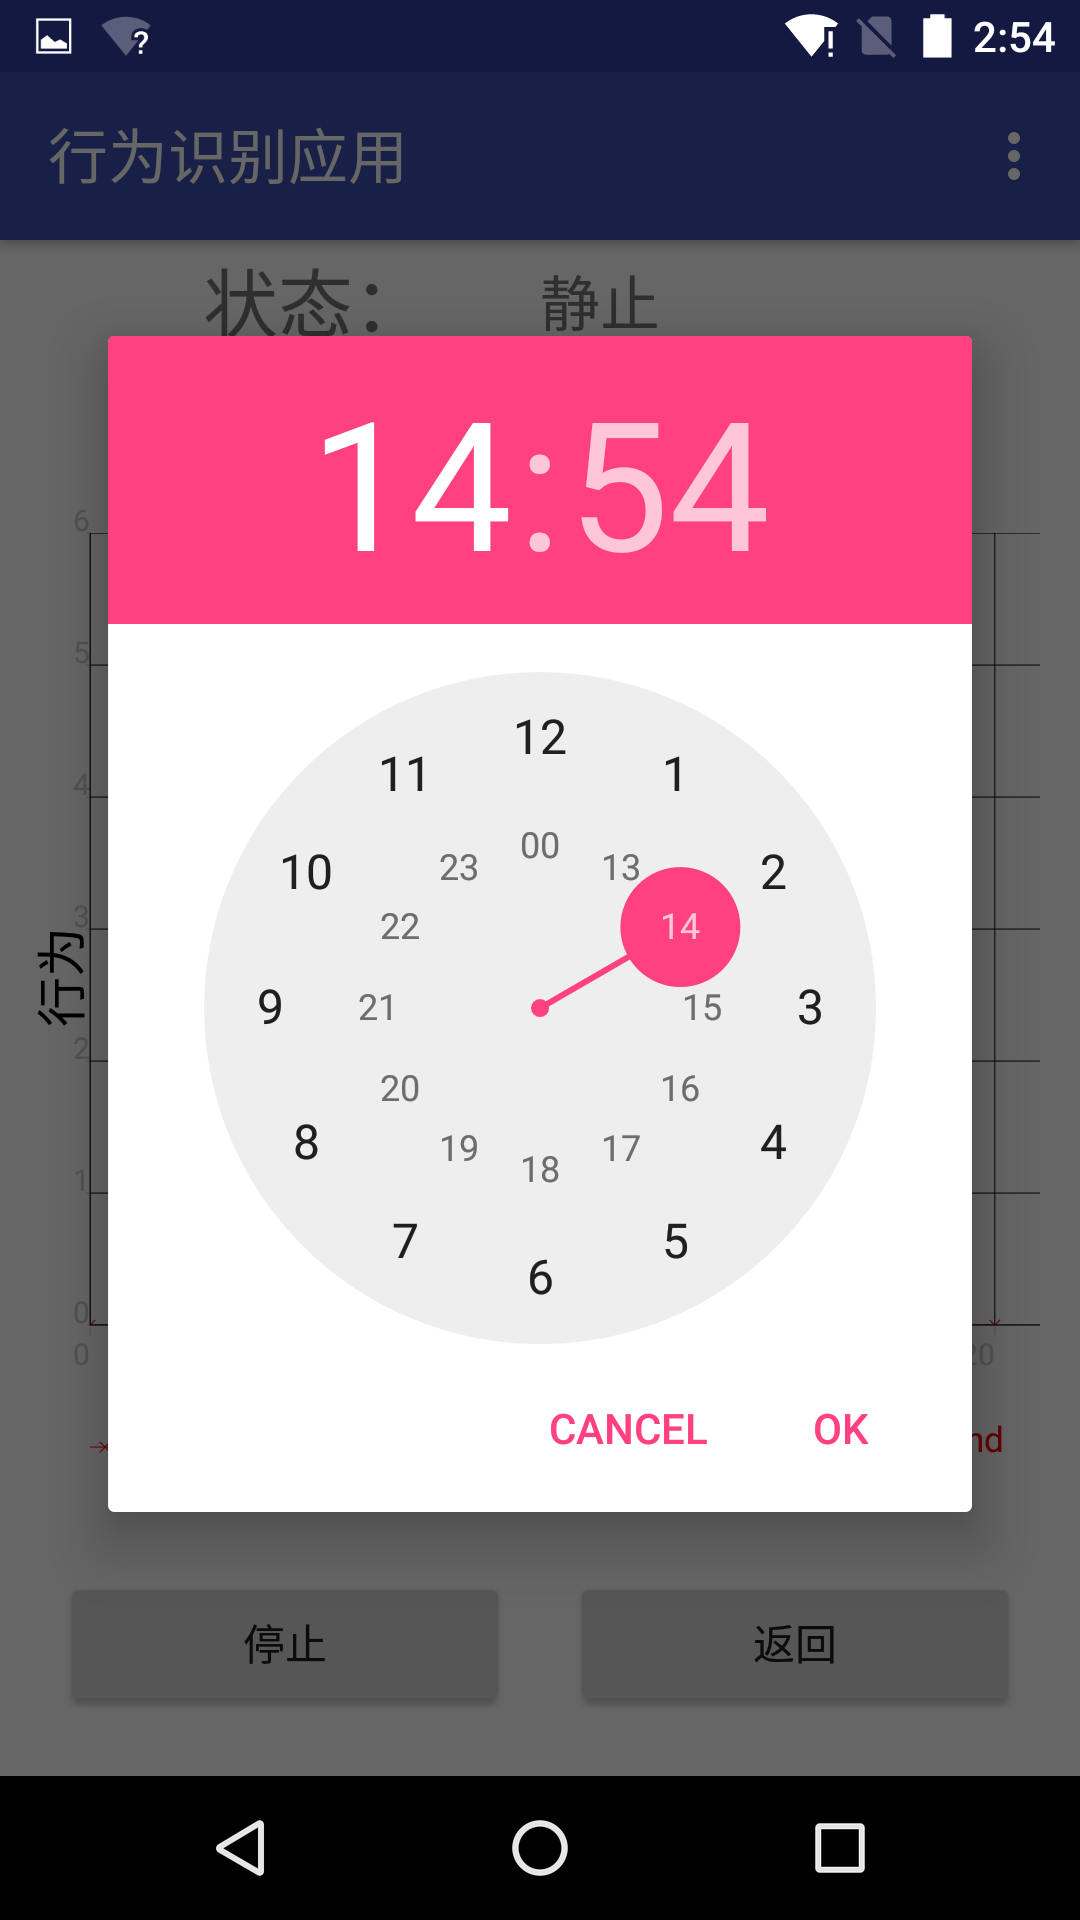
\includegraphics[width=0.23\textwidth]{dialog.png}}
    \caption{行为识别应用的部分界面}\label{screenshot2}
\end{figure}
\section{本章小结}
\par 本章首先介绍了本文所实现的人体行为识别系统的整体框架结构。然后从控制层部分,算法实现部分,模型层部分和视图层部分四个方面详细介绍了移动端行为识别应用的各部分组成和功能。

  \chapter{总结与展望}

\section{工作总结}
\par 基于智能手机进行行为识别,使用方便灵活,便于对用户行为进行长期监测,有利于行为识别应用的推广。但是智能手机存在着方向和位置变化的问题,为此本文提出了一种基于智能手机的两层多策略的行为识别框架。首先将所有行为根据相似度分为若干组,然后针对不同组的行为特点采样对应策略对其进一步分类,最终完成行为分类。同时,为了在保证一定识别准确率的前提下,尽可能降低识别过程中的能量损耗,本文提出了一种最佳策略的动态调整方案,根据手机当前电量以及识别结果,动态调整数据采集和特征提取策略,以达到降低识别过程中能耗的目标。最后为了验证本文所提出方案的有效性和实用性,本文实现了一款可运行于Android操作系统之上的行为识别手机应用,同时该应用可以与远端服务器完成数据通信和交互,形成一套相对较为完善的行为识别系统。
\begin{enumerate}
	\item 为了应对在行为识别过程中智能手机方向和位置的变化问题,本文首先提出了使用自相关函数的特征,通过针对传感器数据各轴向上的自相关函数之和提取特征,从而有效降低因为手机方向变化对行为识别的影响。其次,本文提出了两层多策略的行为识别框架,可将行为分组后再根据不同的行为特点进一步分类,使得特征选择更有针对性。具体地,对于静态行为本文使用识别过渡状态行为的方法判别静态行为,对于动态行为则是通过位置分类器获取位置信息后,使用特定位置数据训练的分类器做最终的行为分类,有效降低了位置对行为识别的影响。
	\item 本文提出了最佳策略的动态调整方法,可以在保证一定识别准确率的前提下尽可能降低识别过程中的能量损耗。为了实现这一目标,本文首先研究准确率和能耗两项指标与若干影响因素的关系,并选定其中较为重要的四个影响因素(采样率,采样时间,是否使用频域特征,是否使用自相关函数特征)作为变量建立数学模型,然后通过实验测量和计算的方法求解数学模型参数,获得两项指标关于这四个变量的函数关系。通过电量作为系数权衡二者关系建立目标函数,进而将求解最佳策略问题转换为求解关于目标函数的最优化问题,并求解后获得每类行为每种电量等级下的最佳策略。最后本文使用一种动态调整的方法,根据手机的当前电量以及识别结果动态调整最佳策略,最终实现降低能耗的目的。
	\item 本文最后介绍了已经实现基于只能手机的行为识别系统,并且从控制层,算法实现,模型层和视图层四个部分详细介绍了手机应用的组成和功能,根据此应用在实际中的识别准确率和能耗说明本文所提出方法的有效性和实用性。
\end{enumerate}	
\section{研究展望}
\par 通过感知人体的运动和环境信息识别用户当前行为,进而为用户提供更为智能化和人性化服务具有十分重要的意义,因此行为识别技术一直受到研究者的广泛关注。本文是从运动类型信息出发,重点为克服位置和方向变化问题,以及降低能耗问题做了深入研究,但是还有一些关于基于智能手机的行为识别本文所没有涉及的问题,可以继续进行深入的研究。主要包括以下几点:
\begin{enumerate}
	\item 日常行为识别:在实际生活中,识别用户的日常行为对于提供智能化服务更有意义,但是日常行为并非只是简单的几类行为,而且行为之间通常是连续的,可能没有明显区分间隔。研究如何定义行为并限定分类的范围,进而识别日常行为会使得行为识别技术更加贴近于实际。
	\item 多人行为:社交网络是一个非常热门的领域,人与人的关系错综复杂却拥有一定的规律性。同时研究多人的行为并理解不同用户行为之间的关系规律,对于行为识别的研究具有很重要的影响。
	\item 其他类型传感器:随着智能手机的不断发展,将会有越来越多的新型传感器集成到智能手机中,可以通过此类传感器获取用户更加丰富的行为信息。与此同时,已经存在但还没有完全普及的传感器如压力传感器,温度传感器等,也将会被集成到越来越多的智能手机中。因此研究使用此类环境信息或其他类型信息的传感器,而不再局限到运动类型传感器对于基于智能手机的行为识别技术将会有很大的帮助。
	\item 传感器的选择:当可选择传感器的范围较为广泛时,就有必要研究选择传感器集合的问题,可研究如何选择合适的传感器集合以适应当前的行为识别,从而在保证准确率的同时减低识别能耗。
\end{enumerate}
%%%%%%%%%%%%%%%%%%%%%%%%%%%%%%
%% 附件部分
%%%%%%%%%%%%%%%%%%%%%%%%%%%%%%
\backmatter

  % 参考文献
  % 使用 BibTeX
  % 选择参考文献的排版格式。注意ustcbib这个格式不保证完全符合要求,请自行决定是否使用
  \bibliographystyle{ustcbib}%{GBT7714-2005NLang-UTF8}
  \bibliography{bib/tex}
  \nocite{*} % for every item
  % 不使用 BibTeX
  % %\renewcommand{\baselinestretch}{0.5}
\begin{thebibliography}{10}

\bibitem{deng:01a}
{邓建松,~彭冉冉,~陈长松邓建松,~彭冉冉,~陈长松邓建松,~彭冉冉,~陈长松邓建松,~彭冉冉,~陈长松邓建松,~彭冉冉,~陈长松邓建松,~彭冉冉,~陈长松邓建松,~彭冉冉,~陈长松邓建松,~彭冉冉,~陈长松邓建松,~彭冉冉,~陈长松邓建松,~彭冉冉,~陈长松邓建松,~彭冉冉,~陈长松}.
\newblock {\em \LaTeXe{}~科技排版指南}.
\newblock 科学出版社,~书号:~7-03-009239-2/TP.1516, 北京, 2001.

\bibitem{wang:00a}
王磊.
\newblock {\em \LaTeXe{}~插图指南}.
\newblock 2000.

\bibitem{zhang:03a}
张林波.
\newblock {\em 关于新版~CCT~的说明}.
\newblock 2003.

\bibitem{lshort-cn}
C\TeX{} 翻译小组.
\newblock {\em lshort~中文版~3.20}.
\newblock 2003.

\bibitem{knuth86e}
Donald~E. Knuth.
\newblock {\em Computer Modern Typefaces}, volume~E of {\em Computers and
  Typesetting}.
\newblock Addison-Wesley, Reading, Massachusetts, 1986.

\bibitem{knuth86d}
Donald~E. Knuth.
\newblock {\em {METAFONT}: The Program}, volume~D of {\em Computers and
  Typesetting}.
\newblock Addison-Wesley, Reading, Massachusetts, 1986.

\bibitem{knuth86c}
Donald~E. Knuth.
\newblock {\em The {METAFONT}book}, volume~C of {\em Computers and
  Typesetting}.
\newblock Addison-Wesley, Reading, Massachusetts, 1986.

\bibitem{knuth86b}
Donald~E. Knuth.
\newblock {\em {TeX}: The Program}, volume~B of {\em Computers and
  Typesetting}.
\newblock Addison-Wesley, Reading, Massachusetts, 1986.

\bibitem{knuth86a}
Donald~E. Knuth.
\newblock {\em The {TeX}book}, volume~A of {\em Computers and Typesetting}.
\newblock Addison-Wesley, Reading, Massachusetts, 1986.

\bibitem{lamport85a}
Leslie Lamport.
\newblock {\em {LaTeX} --- A Document Preparation System: User's Guide and
  Reference Manual}.
\newblock Addison-Wesley, Reading, Massachusetts, 2nd edition, 1985.

\end{thebibliography}


  % 附录,没有请注释掉
 % \begin{appendix}
%    
\chapter{关于硕士、博士学位论文撰写要求}
\label{chap:requires}

学位

\section{对学位论文的基本要求}

\textbf{一下文字仅作示例,一切以学校规定为准!}

\subsection{硕士学位论文}

根据《中华人民共和国学位条例暂行实施办法》第八条的规定,硕士学位论文应能表明作者确已在本门学科上掌握了坚实的基础理论和系统的专门知识,并对所研究的课题有新的见解,有从事科学研究或独立担负专门技术工作的能力。硕士学位论文工作一般是在硕士生完成培养计划规定的课程学习后开始,其工作内容因学科的性质不同而有所差异,一般包括文献阅读、开题报告、拟定并实施工作计划、科研调查、实验研究、理论分析和文字总结等工作。论文正文一般应不少于3万字。硕士学位论文必须有一定的工作量,在论文题目确定后,用于论文工作的时间一般不应少于1.5年。

\subsection{博士学位论文}





\section{本章小结}

%
%  \end{appendix}

  \makeatletter
  \ifustc@bachelor\relax\else
    % 致谢
	%
\begin{thanks}

\par 时光荏苒,岁月如梭,三年紧张而充实的研究生学习生活已经接近尾声,回顾在中国科技大学的这段宝贵的时光,我的内心充满无限的感怀与眷恋。在毕业论文即将完成之际,我要向这三年里所有关心、帮助和鼓励的人致以最真诚的感谢!感谢你们的支持让我在研究生学习阶段在学习、科研和生活方面都受益良多。
\par 首先,感谢我的导师刘斌副教授的谆谆教诲和悉心指导,刘老师耐心地教导我做科研的方法并毫无保留地与我分享他丰富的生活与科研经验,对我的个人成长以及科研工作都具有极大的帮助。在过去的三年,刘老师对我的学习和科研生活倾注了大量精力和心血,为我提供了大量的学习与锻炼的机会,并在我面临生活和科研问题时给予我很大的帮助和鼓励。刘老师知识渊博,治学严谨,并且对科研问题的把我十分到位,总是可以一针见血地指出我科研工作中存在的问题并给予切实可行的解决意见。此外,刘老师深厚而扎实的学识功底、严谨的研究态度、敏锐的洞察力以及宽广的视野与胸怀都使我受益匪浅。在此向刘老师致以最诚挚的谢意!
\par 同时,十分感谢研究生期间其他老师、同学和朋友们的关心和帮助。在此要特别感谢俞能海教授对我的指导和教育。俞老师不仅在科研上给予我以极大的帮助和鼓励,并且在思想觉悟、认知高度和人生职业规划上使我有了全新的认识。此外,还要感谢6系的各位老师们的辛勤教诲,他们使我拥有更加扎实的基础知识以及更加广阔的知识领域认知和理解。同时,还要感谢实验室的兄弟姐妹,他们有已经毕业的师兄师姐包括王明琛、何磊、陈珏、危江月、丰慧、余宿城、罗金国、尤勇、谢宇、吴文超、刘可佳,还有在读的包括邹磊、刘志强、赵孝松、罗浩、云凡、蒋浩然、管程杰、殷国军、金红兴、李航、陈胜、朱辉辉以及大实验室的其他同学,在此还要特别感谢邹磊、余宿城、刘志强和金红兴同学在本文的实验部分给予的支持和帮助。此外,还要感谢306的室友及好友廖鹏、杨卓煦、林阳,谢谢你们的无私帮助。
\par 最后,需要特别感谢的是我的家人。他们一如既往地默默奉献,一直鼓励和支持着我,是我求学道路上最为坚强的后盾。感谢您们的默默付出,感谢您们的支持与帮助,您们对我的无私的爱以及为我营造的宽松的学习环境和氛围使我一生最为宝贵也是最需要去珍惜的财富。
\par 感谢科大,感谢一路走来的兄弟姐妹们,在最宝贵的青春年华里,感激与你们的相遇,感谢你们伴随我的成长。最后为每一位曾经帮助和支持过我的老师、同学和朋友致以最诚挚的谢意!

\vskip 10pt

\begin{flushright}
~~~~郭乾~~~~

\today

\end{flushright}
\end{thanks}
%硕博致谢部分
    % 发表文章目录
    %
\chapter{在读期间发表的学术论文与取得的研究成果}



\noindent\textbf{已发表论文:}

\begin{enumerate}

\item Qian Guo, Bin Liu, Chang Wen Chen. “A Two-layer and Multi-strategy Framework for Human Activity Recognition using smartphone” IEEE ICC 2016 SAC E-Health (ICC 2016).
\end{enumerate}

\vskip 1cm


    \fi
  \makeatother



\end{document}
